\documentclass[12pt]{article}
\usepackage[spanish, english, es-tabla]{babel}
\usepackage[utf8]{inputenc}
\usepackage[left = 2cm, right = 2cm, bottom = 2cm, top = 3cm]{geometry}
\usepackage{amsmath, amssymb}
\usepackage{graphicx}
\usepackage{hyperref}
\usepackage{listings}
\usepackage{courier}

\usepackage[dvipsnames]{xcolor}

% Portada Oficial
\usepackage[export]{adjustbox}

\renewcommand{\lstlistingname}{Ejemplo}
\renewcommand{\lstlistlistingname}{Listado de ejemplos}

% https://tex.stackexchange.com/questions/60209/how-to-add-an-extra-level-of-sections-with-headings-below-subsubsection
\newcommand{\subsubsubsection}[1]{\paragraph{#1}\mbox{}\\}
\setcounter{secnumdepth}{4}
\setcounter{tocdepth}{4}

% Configuracion PDF metadata
\hypersetup{
	pdftitle= {Aplicación de técnicas de virtualización ligera para la evaluación de redes de comunicaciones},
	pdfauthor = {Enrique Fernández Sánchez},
	pdfsubject = {Simulación de redes utilizando namespaces},
	pdfkeywords = {NFV, SDN, Linux, namespaces, containers, Docker, LXC, mininet, OpenSource}
}

% Configuracion colores hiperenlaces
\hypersetup{
	colorlinks=true,
	linkcolor=black,
	%filecolor=magenta,      
	urlcolor=cyan,
}

% Configure lstlisting
\definecolor{codegreen}{rgb}{0,0.6,0}
\definecolor{codegray}{rgb}{0.5,0.5,0.5}
\definecolor{codepurple}{rgb}{0.58,0,0.82}
\definecolor{backcolour}{rgb}{0.95,0.95,0.92}

\lstdefinestyle{mystyle}{
	backgroundcolor=\color{backcolour},   
	commentstyle=\color{codegreen},
	keywordstyle=\color{magenta},
	numberstyle=\tiny\color{codegray},
	stringstyle=\color{codepurple},
	basicstyle=\ttfamily\footnotesize,
	breakatwhitespace=false,         
	breaklines=true,                 
	captionpos=t,                    
	keepspaces=true,                 
	numbers=left,                    
	numbersep=5pt,                  
	showspaces=false,                
	showstringspaces=false,
	showtabs=false,                  
	tabsize=2
}

\lstset{style=mystyle}

% Configuracion encabezados y pies de pagina
\usepackage{fancyhdr}
\fancyhf{}
\lhead[\leftmark]{\small TFE: Enrique Fernández Sánchez}
\rhead[Nombre Autor]{\rightmark}
\cfoot[\thepage]{}
\cfoot[]{\thepage}
\renewcommand{\headrulewidth}{0.5pt}
\renewcommand{\footrulewidth}{0pt}
\fancypagestyle{plain}{
	\fancyhf{}
	\fancyhead[L]{\small TFE: Enrique Fernández Sánchez}
	\fancyfoot[C]{\thepage}
	%\renewcommand{\headrulewidth}{0pt}		% Sirve para eliminar linea
	%\renewcommand{\footrulewidth}{0pt}		% Sirve para eliminar linea
}
\pagestyle{fancy}

\begin{document}
	\selectlanguage{spanish}
	
	%%%% PORTADA V1
	%\title{\textbf{Aplicación de técnicas de virtualización ligera para la evaluación de redes de comunicaciones} \\ 
	%\addvspace{10px} \large \textit{Trabajo Final de Estudios} \\
	%\large Ingeniería Telemática}
	%\author{Autor: Enrique Fernández Sánchez \\ Tutor: Josemaria Malgosa Sanahuja \\ \\Universidad Politécnica de Cartagena}
	
	%% EDITAR PARA SEGUIMIENTO DE VERSIONES
	%\date{Revisión Enero 2022}
	
	%\maketitle
	%\pagebreak
	%%% END PORTADA
	
	%% PORTADA UPCT
	\thispagestyle{empty}
	
	\newgeometry{left=0.01cm, bottom=0.01cm, top=0.01cm}

	\begin{minipage}{0.2\textwidth}
		
\includegraphics[height=\textheight, left]{img/banda_etsit_90.png}
	\end{minipage}
	\centerline{\begin{minipage}[t][5cm][b]{0.5\textwidth}
		\title{\textbf{Aplicación de técnicas de virtualización ligera para la evaluación de redes de comunicaciones}} 
		
		%% EDITAR PARA SEGUIMIENTO DE VERSIONES
		\date{Revisión Febrero 2022}
		
		\maketitle
	
		\vspace{0.5cm}
	
		\hspace{1.5cm} \textbf{TRABAJO FIN DE GRADO} \\
	
		\vspace{0.5cm}
	
		\hspace{1.8cm} Grado en Ingeniería Telemática \\
	
		\vspace{1cm}
	
		\textbf{Autor:}\author{ Enrique Fernández Sánchez}\\
	
		\textbf{Tutor:} Josemaria Malgosa Sanahuja
	\end{minipage}}

	\restoregeometry
	%% END PORTADA UPCT	
	
	\pagebreak
	
	\tableofcontents
	
	\pagebreak
	
	\addcontentsline{toc}{section}{Índice de figuras}
	\listoffigures
	
	\pagebreak
	
	%\addcontentsline{toc}{section}{Índice de tablas}
	%\listoftables
	
	\addcontentsline{toc}{section}{Listado de ejemplos}
	\lstlistoflistings
	
	\pagebreak
	
	%%% Glosario
	\pagebreak
	\section*{Glosario de términos}
	\addcontentsline{toc}{section}{Glosario de términos}
	\thispagestyle{plain}
	
	%\noindent{\large \textbf{NFV}} (\textit{Network Function Virtualization}). Virtualización de funciones de red.\\
		 
	%\noindent{\large \textbf{SDN}} (\textit{Software Defined Networks})\\
		 
	%\noindent{\large \textbf{Namespace}}. \textit{Espacio de nombres}\\
		 
	%\noindent{\large \textbf{NS}} (\textit{Network namespace}). Tipo de espacio de nombres en Linux que tiene por función aislar la parte de red de la máquina host.\\
	
	\noindent{\large \textbf{Linux}}. Sistema operativo tipo UNIX, de codigo abierto, multiplataforma, multiusuario y multitarea.\\
	
	\noindent{\large \textbf{Unix}}. Sistema operativo portable, multitarea y multiusuario desarrollado a partir de 1969. Se divide en tres tareas básicas: el nucleo de sistema operativo, el interprete de comandos y programadas de utilidades.  \\
		 
	\noindent{\large \textbf{Kernel de Linux}}. Núcleo del sistema operativo Linux.\\
		 
	\noindent{\large \textbf{PID}} (\textit{Process Identifier}). Identificador de procesos que están ejecutándose bajo un sistema tipo Linux.\\
	
	\noindent{\large \textbf{UID}} (\textit{User identifier}). Encontrado normalmente como un número o palabra, supone un identificador de usuario dentro del sistema Linux.\\
	
	\noindent{\large \textbf{GID}} (\textit{Group Identifier}). Al igual que sucede con el UID, suele aparecer como un número o palabra y hace referencia al identificador de grupo dentro del sistema de Linux.\\
		 
	\noindent{\large \textbf{root}}. Cuenta superusuario del sistema operativo Linux.\\
		 
	%\noindent{\large \textbf{veth-pair}} (\textit{Virtual Ethernet Pair}). Tipo de interfaz virtual. Funcionan de dos en parejas.\\
	
	\noindent{\large \textbf{NAT}} (\textit{Network Address Translation}). Traducción de direcciones de red, mecanismo utilizado por router para cambiar paquetes entre redes con direcciones IP diferentes.\\
	
	\noindent{\large \textbf{DHCP}} (\textit{Dynamic Host Configuration Protocol}). Protocolo de red que permite a un servidor asignar dinámicamente direcciones IP y otros parámetros, a cada dispositivo de la red en la que se encuentre. \\
	
	\noindent{\large \textbf{API}} (\textit{Application Programming Interface}). Conjunto de subrutinas, funciones y procedimientos que ofrecen cierto software, con el objetivo de ser utilizado por otro software externo.
		 
	
	\pagebreak
	
	%%% TODO
	\section*{Agradecimientos}
	\addcontentsline{toc}{section}{Agradecimientos}
	\thispagestyle{plain}
	
	\noindent En primer lugar, agradecer a mi tutor, Josemaria Malgosa Sanahuja, por presentarme este proyecto y animarme en todo momento para su realización. Agradezco mucho su tiempo, su dedicación y su ayuda, que han sido una parte clave para la realización de este trabajo.
	
	\noindent Por otro lado, me gustaría agradecer a mi familia, en especial a mis padres, Encarni y Miguel Ángel, y a mi hermano, Miguel; ellos han supuesto una parte fundamental de mi apoyo en este camino que ha sido la ingeniería, ellos han sido mi principal apoyo, y sin él, no hubiera llegado hasta donde estoy hoy. También agradecer a mis padrinos, Ana y Tasio, ya que siempre han tenido palabras de ánimo para mi. Especial mención a mis abuelos, estoy seguro que estarían orgullosos de mi camino y de como su nieto es ahora ingeniero. Agradecer también a mis suegros, María Dolores y Francisco, ya que suponen otra fuente de apoyo y confianza.
	
	\noindent Especial mención a Lucía Francoso Fernández, compañera del grado en sistemas de telecomunicación, con la cual he tenido la suerte de emprender codo con codo muchos de los proyectos que he llevado entre manos estos años. Fuente de apoyo incondicional, una mina de creatividad y una brillante ingeniera. 
	
	\noindent Por último agradecer a mis compañeros del \textit{Free Open Source Club}, ya que gracias a ellos he podido valorar el movimiento \textit{Open Source}, y servirme de trampolín para entrar a un mundo muy bonito del conocimiento libre. 
		
	\pagebreak
	
	\section{Introducción}
	\noindent Con el fin de concluir los estudios de grado en ingeniería telemática, es necesaria la investigación y el posterior desarrollo del \textit{Trabajo Fin de Estudios} (TFE). Dicho trabajo, tiene como objetivo enfrentar al alumno a un proceso de investigación en el que pueda aplicar los conceptos que ha ido aprendiendo durante su paso por el grado, además pudiendo añadir puntos de innovación, y aportar soluciones nuevas a un proyecto en específico.\\
	
	\noindent En este documento, recojo lo que sería mi memoria en relación al TFE. En dicho documento detallaremos las diferentes investigaciones realizadas sobre el concepto de virtualización en sistemas Linux, como funcionan los contenedores y como utilizar la virtualización ligera para la evaluación de redes de comunicaciones, en nuestro caso, de conmutación de paquetes. \\
	
	\noindent Además, toda documentación y códigos utilizados en este proyectos se ha liberado en un repositorio de \textit{GitHub} (\url{https://github.com/}). En dicho repositorio, encontraremos toda la información recopilada para este trabajo, además de los códigos fuente de la memoria, y las pruebas realizadas. La dirección del repositorio es la siguiente: \url{https://github.com/Raniita/lightweight-virtualization-nfv/}
	
	\subsection{Contexto del trabajo}
	\noindent Este proyecto nace con el objetivo de profundizar en conceptos novedosos para el ámbito de red, como por ejemplo podría ser NFV. Definimos NFV (Network Function Virtualization) como la virtualización de hardware físico de red, con el fin de solucionar problemas de escalabilidad y de optimización.\\
	
	 \noindent Además, trabajaremos sobre otras tecnologías igual de importantes como pueden ser la virtualización de recursos, o los bien conocidos \textit{contenedores}. Particularizaremos estas tecnologías y las acercamos al campo de conocimiento de la telemática para utilizarlas con el fin de evaluar y simular redes de conmutación de tipo IP. \\
	
	\noindent Partiendo de supuesto de que las herramientas más sencillas de simulación de redes se nos pueden quedar cortas en cuanto queremos escalar el sistema, nos topamos en que otras soluciones pueden ser mucho más \textit{resource hungry} de lo que podríamos imaginar. Además, tampoco podemos contar con realizar dichas pruebas de manera física, ya que el presupuesto del proyecto escalaría de nivel exponencial. Esto sucede ya que deberíamos configurar cada dispositivo de manera específica, y después proceder a interconectarlos con una tecnología de red adecuada, que en nuestro caso, son tecnologías en fase de desarrollo o evaluación de prestaciones.\\
	
	%\noindent Conociendo las limitaciones, establecemos una serie de objetivos de cara a evaluar el viaje que realicemos durante ese proyecto, y poder evaluar posteriormente los avances que hemos podido conseguir, y además las conclusiones vinculadas a estos. Estos objetivos podrían ser:\\
	%\begin{itemize}
	
	\pagebreak
	
	\subsection{Objetivos}
	\noindent Como bien hemos adelantado en el apartado anterior, el objetivo principal de este proyecto es el de analizar la situación en el ámbito de simulación y evaluación de redes de comunicación, además, concretar en aquellas soluciones que estén basadas en virtualización ligera. Por lo tanto, se pretende: 
	\begin{itemize}
		\item Aprender los conceptos básicos de la virtualización de sistemas de red (\texttt{NFV}).
		\item Comprender la diferencia entre virtualización \textit{ligera} y virtualización ``\textit{dura}''.
		\item Estudiar, dentro del sistema operativo Linux, las diferentes tecnologías que nos permiten adoptar soluciones \texttt{NFV}.
		\item Definir que es espacio de nombres y como podemos aplicarlo para virtualizar redes.
		\item Profundizar en el concepto de interfaces virtuales en Linux.
		\item Desgranar el concepto amplio de contenedor, relacionándolo con los espacios de nombres.
		\item Aportar una serie de ejemplos que puedan servir de guía para la evaluación de redes de comunicaciones, utilizando virtualización ligera.
	\end{itemize}

	\subsection{Descripción de los capítulos restantes de la memoria}
	\noindent En este apartado se comentará brevemente la distribución de capítulos de la memoria. Además, se mencionará que temas se han abordado en cada uno de ellos.
	\begin{itemize}
		\item \textbf{Capítulo 1}: \textit{Introducción}. Comienzo del proyecto. Se exponen introducción, objetivos y el contexto del trabajo. \\
		
		\item \textbf{Capítulo 2}: \textit{Virtualización de funciones de red}. Se pretende contextualizar el porqué es importante la virtualización de las redes. Además, se comenta sobre las tecnologías involucradas para dar lugar a la virtualización. \\
		
		\item \textbf{Capítulo 3}: \textit{Interfaces de red virtuales en Linux}. Se comentará las diferentes interfaces de red virtuales que nos ofrece Linux. Se evaluarán sus ventajas y como nos pueden ser útiles para implementar topologías de red virtualizadas. \\
		
		\item \textbf{Capítulo 4}: \textit{Espacio de nombres en Linux}. Se estudiará el concepto de espacio de nombres. Se aportará una explicación de cada espacio de nombres disponibles, además de ejemplos de aplicación de los más importantes. \\
		
		\item \textbf{Capítulo 5}: \textit{Virtualización ligera y contenedores}. Se profundiza en diferentes técnicas de virtualización ligera, además de proponer ejemplos y primeros pasos para cada una de las soluciones propuestas. \\
		
		\pagebreak
		
		\item \textbf{Capítulo 6}: \textit{Caso práctico: Virtualización para la simulación de redes}. Se proponen varios ejemplos de \textit{software} en el que se utiliza virtualización ligera para la simulación de redes. \\
		
		\item \textbf{Capítulo 7}: \textit{Conclusiones}. Se muestran las conclusiones obtenidas, tanto de puntos en especifico, como de la totalidad del trabajo. Además, se proponen lineas de investigación futuras. \\
	\end{itemize}
	
	
	\pagebreak
	
	\section{Virtualización de Funciones de Red}
	\label{sec: nfv}
	%% https://www.youtube.com/watch?v=3JEAK66wujg	
	\noindent El punto de partida de la ``virtualización de funciones de red'' (\texttt{NFV}) surge a partir de las necesidades de las operadoras de red para solucionar los problemas de gran escala de la red. Estos problemas se pueden resumir en los siguientes:
	\begin{itemize}
		\item Saturación general en la red, o bien en servicios específicos.
		\item Servicios que requieren una instalación manual o que necesitan una intervención manual.
		\item Problemas relacionados con las operadoras de red, como puede ser la reducción de costes del servicio.
	\end{itemize}
	
	\noindent Estos problemas radican en una serie de motivos, pero principalmente tiene que ver con el poco crecimiento de la red, y la rápida adopción por la sociedad. Si concretamos estos motivos, podrían ser tal que:
	\begin{itemize}
		\item Falta de estabilidad en la red, debido a la poca flexibilidad de la misma.
		\item Poca evolución en las redes ``core''.
		\item Falta de innovación, se hace realmente difícil crear nuevos servicios.
	\end{itemize}

	\noindent En general, se podría resumir en que la poca innovación y la falta de flexibilidad, hacían realmente difícil cambiar ciertos servicios y estructuras críticas de la red ``core''. Para ello, para solucionar todos estos problemas, desde los grupos de trabajo de la ITU se empezó a trabajar en nuevas propuestas con el fin de aportar nuevas alternativas. La solución propuesta con más apoyo sería ``la virtualización de funciones de red'', que tendría su punto de partida en octubre de 2012, en un grupo de trabajo de la ITU, formado por 13 operadoras internacionales, dando lugar a un \textit{paper} informativo [\ref{paper nfv 2012}] en el que se detallaba de forma teórica la solución de \texttt{NFV}. \\
	
	\noindent En esta arquitectura de red basada en virtualización, distinguimos varios roles: 
	\begin{itemize}
		% https://www.redhat.com/es/topics/cloud-native-apps/vnf-and-cnf-whats-the-difference
		\item \texttt{VNF} (\textit{Virtual Network Function}). Aplicaciones software que ofrecen ciertas funciones (enrutadores, firewall...) y que se implementan como máquinas virtuales, y que no necesitan un sistema hardware en específico. 
		
		% https://www.sdxcentral.com/networking/nfv/definitions/nfv-infrastructure-nfvi-definition/
		\item \texttt{NFVi} (\textit{NFV infraestructure}). Se trata de la infraestructura disponible para una arquitectura basada en NFV. Supone la infraestructura donde se desplegarán los \texttt{VNF}, que incluye recursos de computo, almacenamiento y de red. 
		
		% https://www.sdxcentral.com/networking/nfv/definitions/virtualized-infrastructure-manager-vim-definition/
		\item \texttt{VIM} (\textit{Virtualized Infraestructure Manager}). Es el elemento responsable de controlar y gestionar la infraestructura \texttt{NFV} (NFVi). Se encarga de mantener el inventario de recursos y como ir ``colocando'' las diferentes funciones de red en los recursos disponibles de la red. Esto nos permite realizar tareas de orquestación.
		
		% https://www.adva.com/en/products/technology/what-is-nfv-mano
		\item \texttt{MANO} (\textit{Management and orchestration}). Elemento clave para la implementación de \texttt{NFV}. Es el encargado de coordinar los recursos de la red y gestionar las funcionalidades de red. Esta compuesto por los elementos: orquestador NFV (NFVO), gestor de VNF (VNFM) y gestor de infraestructura virtualizada (VIM).
	\end{itemize}
	
	\pagebreak
	
	\noindent En la actualidad, cada dispositivo/funcionalidad se corresponde con un aparato físico. Estos son dispositivos son embebidos y solo cumplen una función específica (firewall, balanceador de carga, router...). Utilizando la virtualización de red (\texttt{NFV}), podemos llegar al punto de tenerlo todo virtualizado. Teniendo una ``imagen'' de router, la podemos desplegar en cualquier ordenador de carácter general, y cumplir diferentes funciones a la vez (que un router sea a la vez un firewall, por ejemplo). \\
	
	\begin{figure}[h]
		\begin{center}
			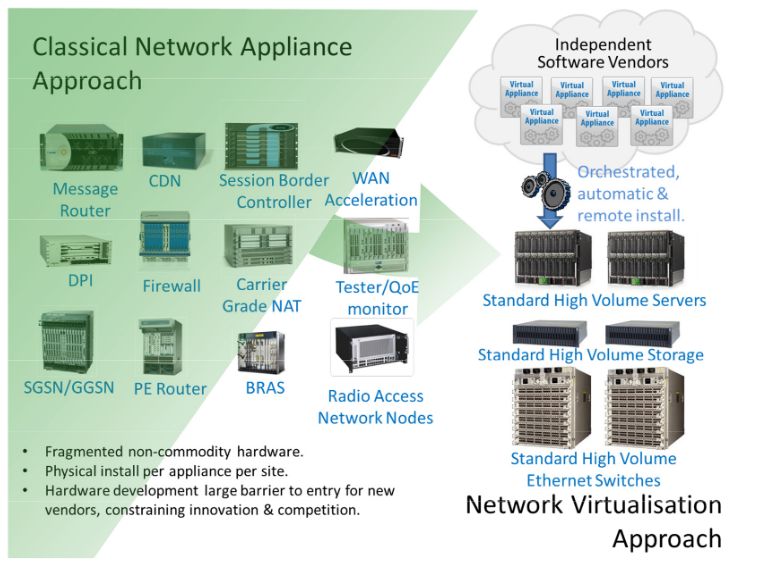
\includegraphics[width=0.8\textwidth]{img/classic_network_vs_nfv.png}
			\label{imagen comparativa classic network nfv}
			\caption{Comparativa enfoque clásico de las redes contra el enfoque virtualizado. [\ref{img: nfv vs classic}]}
		\end{center}
	\end{figure}
	
	\noindent En el enfoque clásico, las funciones de red están basadas en tener un software y hardware específico para cada dispositivo. Sin embargo, \texttt{NFV} nos aporta que esos recursos software y hardware, se despliegan en servidores físicos de propósito general, dando lugar a una mejor gestión de los recursos y un mayor aprovechamiento. Por lo tanto, un mismo nodo físico, puede ser DHCP, router o Firewall. [\ref{bib: what is nfv}]\\
	
	\pagebreak

	\noindent La virtualización de funciones de red supone una manera para reducir costes y acelerar el desarrollo de servicios para los operadores de red a costa de desacoplar funciones como pueden ser un ``firewall'' en un hardware dedicado, moviendolos a servidores virtuales. \\ 
	
	\noindent Tal y como podemos ver en la comparativa de la Figura \ref{img: comparativa redes classic vs nfv}, sustituimos electrónica de red específica, como podrían ser router, switches, etc; por máquinas virtualizadas que se despliegan en servidores de carácter general, dando lugar a un mayor control y escalabilidad de los sistemas físicos. A consecuencia de esto, podemos ver como las redes toman un camino diferente, dejando a atrás el hardware y software propietario, para centrarse en un enfoque basado en el software. \\
	
	\begin{figure}[h!]
		\begin{center}
			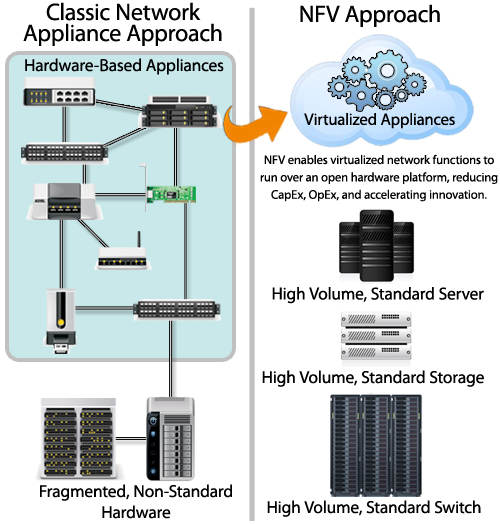
\includegraphics[width=0.6\textwidth]{img/NFV-image-v2.jpg}
			\label{img: comparativa redes classic vs nfv}
			\caption{Comparativa redes clásicas vs redes basadas en NFV [\ref{img: nfv vs classic 2}]}
		\end{center}
	\end{figure}
	
	\pagebreak
	
	\subsection{Tecnologías implicadas}
	\noindent Para que este cambio de paradigma en las redes se materialice y que pasen a ser una solución viable, tienen que realizarse una serie de desarrollos, los cuales provocan que aún a día de hoy sean soluciones experimentales, que aunque son utilizadas en entornos reales, todavía están en continuo desarrollo e investigación. \\
	
	\noindent Además, aunque estamos hablando de NFV, hay una tecnología extra que también aparece en la ecuación, esta tecnología es SDN (\textit{Software Defined Networks}). En este caso particular, nos encontramos con que el NFV no puede existir sin el SDN, y viceversa [\ref{bib: sdn y nfv}]. Si tuviéramos que definir brevemente cada una de dichas tecnologías, podríamos resumirlo en lo siguiente:
	\begin{itemize}
		\item \textit{Software Defined Networks} (\texttt{SDN}). Desacoplo del plano de control de los dispositivos de una red. Aparece la figura de controlador SDN que permite ``controlar'' la red via software. Para ello, se utiliza una API de control (\texttt{Southbound API}), con el fin de dirigir el tráfico de red y comunicarse con la infraestructura hardware de capas superiores. (ver Figura \ref{img: sdn + nfv})
		 
		\item \textit{Network Functions Virtualizations} (\texttt{NFV}). NFV desacopla las funciones de la red de dispositivos de hardware dedicados y las traslada a servidores virtuales, y así se consolidan múltiples funciones en un único servidor físico. Dentro de este servidor físico, podemos distinguir diferentes funciones de red virtuales (VNF), dichas funciones suponen un conjunto de máquinas interconectadas entre sí, y cada una de ellas tiene una función distinta, y además, el conjunto de ellas tienen por objetivo realizar una función que antes era realizada por un equipo físico determinado (un router, firewall o similar). Aporta una API para controlar los diferentes dispositivos virtuales (\texttt{Northbound API}) (ver Figura \ref{img: sdn + nfv})
	\end{itemize}

	\begin{figure}[h!]
		\begin{center}
			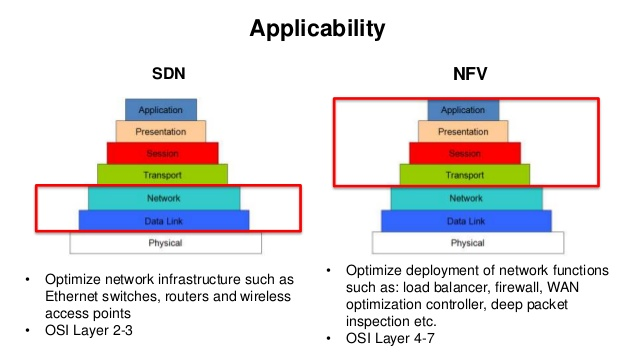
\includegraphics[width=0.85\textwidth]{img/sdn-y-nfv.jpg}
			\caption{Comparativa en capas OSI de las tecnologías NFV y SDN [\ref{img: sdn vs nfv osi}] }
			\label{img: sdn + nfv}
		\end{center}
	\end{figure}

	\pagebreak
	
	\subsection{Virtualización ligera}
	\label{sect: virt ligera}
	
	\noindent Entendemos la virtualización ligera como un tipo de virtualización de un sistema. Dicha virtualización se hace a nivel de sistema operativo, aportando que existan diferentes espacios de usuarios aislados entre sí, sin embargo, a diferencia del concepto ``\textit{máquina virtual}'' (virtualización dura), en la virtualización ligera todos los sistemas virtualizados dependen del \texttt{kernel} de la máquina host, mientras que en el caso de una máquina virtual (virtualización tipo 1 y 2), cada instancia tendría su propio \texttt{kernel} (ver Figura \ref{img: virtualization comparative}). [\ref{bib: virt ligera}]\\
	
	\noindent Por lo tanto, las ventajas destacables sobre la virtualización ligera frente a la virtualización ``dura'' (virtualización de tipo 1 y 2) serían:
	\begin{itemize}
		\item Un único \texttt{kernel} para todas las instancias que queramos ejecutar.
		\item Eliminamos el correspondiente \textit{overhead} al no tener que emular un \texttt{kernel} para cada instancia.
		\item Menor consumo de CPU y RAM, comparado con las virtualizaciones ``duras''.
		\item Disponen de la posibilidad de iniciar, mover, parar o borrar la instancia virtualizada.
	\end{itemize}
	
	\begin{figure}[h!]
		\begin{center}
			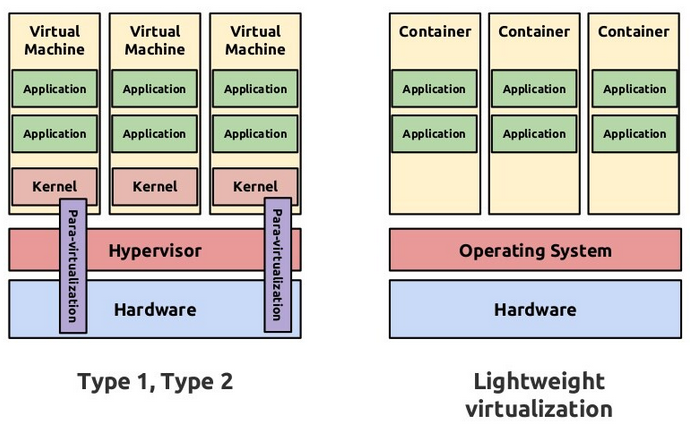
\includegraphics[width=0.8\textwidth]{img/virtualization_comparative.png}
			\caption{Comparativa entre virtualización ligera y virtualización dura [\ref{bib_img: comparativa virt}] }
			\label{img: virtualization comparative}
		\end{center}
	\end{figure}
	
	% Introducción a los siguientes capítulos
	\noindent En consecuencia de tener que utilizar un mismo \texttt{kernel} para todas las instancias, tenemos que profundizar sobre los conceptos de interfaces de red virtuales [\ref{sect: interfaces virtuales}] y espacios de nombres [\ref{sect: espacio nombres}], ya que serán piezas clave para tener nuestras instancias aisladas entre sí, pero a su vez conectadas con los diferentes recursos en red que nosotros definamos.
	
	\pagebreak
	
	\section{Interfaces de red virtuales en \textit{Linux}}
	\label{sect: interfaces virtuales}
	\noindent En este capítulo, vamos a profundizar en el concepto de interfaces de red virtuales, pero las específicas al sistema operativo basados en el kernel de Linux. \\
	
	\noindent Linux dispone de una selección muy diferente de interfaces de red que nos permiten, de manera sencilla, el uso de máquinas virtuales o contenedores. En este apartado vamos a mencionar las interfaces más relevantes de cara a la virtualización ligera que proponemos para el despliegue de una red virtualizada. Para obtener una lista completa de las interfaces disponibles, podemos ejecutar el siguiente comando \texttt{ip link help}.\\
	
	\par \noindent En este trabajo, vamos a comentar la siguientes interfaces [\ref{bib:virtual interface list}]:
	\begin{itemize}
		\item MAC compartida: enp2s0:\{0,1,2...\}
		\item VLAN 802.1q: enp2s0.\{0,1,2...\}
		\item VLAN 802.1ad: enp2s0.\{0,1,2...\}.\{0,1,2...\}
		\item Pares de ethernet virtuales (\textit{veth pairs})
		\item TUN/TAP
	\end{itemize}


	\subsection{Nombres predecibles en dispositivos físicos.}
	%\noindent \% Comentar udev (dinamic device management) \% \\
	\noindent Con el fin de comprender como se nombran las diferentes interfaces de red, es necesario que estudiemos el servicio \texttt{udev} (\textit{Dynamic device management}). \texttt{udev} es el gestor de dispositivos que utiliza el kernel de Linux, su función principal es permitir al administrador del sistema operativo registrar manejadores del espacio de usuario para eventos del sistema. Estos eventos que recibe el servicio \texttt{udev} son principalmente generados por el kernel, en respuesta a eventos físicos relacionados con dispositivos periféricos. Por lo tanto, el propósito de \texttt{udev} es actuar sobre la detección de periféricos y con conexiones tipo \textit{hotplug}, pudiendo encadenar acciones necesarias que devuelven el control al kernel, como por ejemplo, cargar módulos específicos o un firmware de un dispositivo. [\ref{bib: udev archwiki}] \\
	
	\noindent Además, \texttt{udev} también se encarga de gestionar los nodos de dispositivos en el directorio \texttt{/dev} añadiendo, enlazando simbólicamente y renombrándolos. Por otro lado, una consideración a tener en cuenta es que \texttt{udev} maneja los eventos de manera concurrente, lo que aporta una mejora de rendimiento, pero a la vez puede dar problemas a la hora de que el orden de carga de los módulos del kernel no se conserva entre los arranques. Un ejemplo de esto podría ser que en el caso de tener dos discos duros (uno llamado \texttt{/dev/sda} y otro \texttt{/dev/sdb}), en el siguiente arranque el orden de de arranque puede variar, generando que ambos identificadores se intercambien entre sí, desencadenando una serie de problemas en nuestro sistema. [\ref{bib: udev archwiki}]\\
	
	\pagebreak
	
	% Captura de regla udev modificada por usuario
	\noindent A modo de ejemplo, el usuario puede crear sus propias reglas, de modo que puede realizar las acciones que ya hemos comentado, de acuerdo a sus propias necesidades. A modo de ejemplo, podemos ver en la siguiente captura (Figura \ref{img: udev rule}) como hemos creado un archivo en la ruta \texttt{/etc/udev/rules.d/} en el que definimos la regla para un dispositivo físico en específico (en este caso un USB). Identificamos el dispositivo que queremos a través de los atributos \texttt{idVendor} e \texttt{idProduct} (atributos necesarios para cualquier dispositivo USB), después le asignamos un "MODE" que corresponde con los permisos que le queremos asignar al dispositivo (en modo numérico) y el grupo al que permitimos acceder al dispositivo.\\
	
	\begin{figure}[h!]
		\begin{center}
			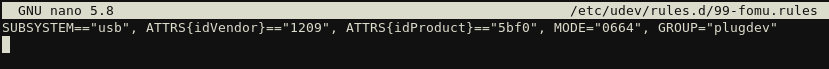
\includegraphics[width=1\textwidth]{img/udev_rule.png}
			\caption{Regla \texttt{udev} definida por el usuario} 
			\label{img: udev rule}
		\end{center}
	\end{figure}
	
	% Comentamos el cambio en el nombrado de las interfaces de red 
	\noindent En el caso de las interfaces físicas de red, vamos a suponer que estamos utilizando el nombrado de interfaces de red antiguo. Esto proviene de que en la últimas versiones del kernel, se ha cambiado la forma en la que las interfaces de red son nombradas por Linux (\texttt{systemd networkd v197} [\ref{bib: systemd networkd v197}]). Es por esto por lo que antes podíamos tener interfaces tal que \texttt{eth0} y ahora nos encontramos con la siguiente nomenclatura \texttt{enps30}. Este cambio surge ya que anteriormente se nombraban las diferentes interfaces conforme el propio ordenador estaba en la etapa de \texttt{boot}, por lo que podría pasar que a lo que nosotros entendíamos como \texttt{eth1}, en el próximo arranque fuera \texttt{eth0}, dando lugar a incontables errores en el sistema. Es por esto por lo que se empecó a trabajar en soluciones alternativas. Por ejemplo, la que acabamos de comentar, utiliza la información aportada por la BIOS del dispositivo para catalogarlo en diferentes categorías, con su formato de nombre para cada categorías. Dichas clasificación corresponde con las siguientes:
	\begin{enumerate}
		\item Nombres incorporados en Firmware/BIOS que proporcionan un número asociado a dispositivos en la placa base. (ejemplo: \texttt{eno1})
		\item Nombres incorporados en Firmware/BIOS proveniente de una conexión PCI Express hotplug, con número asociado al conector. (ejemplo: \texttt{ens1})
		\item Nombres que incorporan una localización física de un conector hardware. (ejemplo: \texttt{enp2s0})
		\item Nombres que incorporan una la MAC de una interfaz. (ejemplo: \texttt{enx78e7d1ea46da})
		\item Sistema clásico e impredecible, asignación de nombres nativa del kernel. (ejemplo: \texttt{eth0})
	\end{enumerate}
	
	\pagebreak
	
	\subsection{MAC compartida: \texttt{enp2s0:\{0,1,2...\}}}
	\par \noindent Todas las interfaces asociadas comparten la misma dirección MAC. Cada una de ellas, recibe el nombre de \textit{aliases}. La funcionalidad principal que tienen este tipo de interfaces es la de asignar varias direcciones de IP a una misma interfaz de red.
	
	\begin{verbatim}
$ ip addr add 192.168.56.151/24 broadcast 192.168.56.255 dev enp2s0 
label enp2s0:1
	\end{verbatim}

	\par \noindent Sin embargo, el comando \texttt{iproute2} admite esta misma funcionalidad sin tener que crear interfaces de red extra. Para ello, solo tenemos que asociar cada IP con la interfaz de red deseada.
	\begin{verbatim}
$ ip addr add 192.168.56.151/24 dev enp2s0
$ ip addr add 192.168.56.251/24 dev enp2s0
	\end{verbatim}

	\subsection{VLAN 802.1q: \texttt{enp2s0.\{0,1,2...\}}}
	\par \noindent Siguiendo el mismo concepto que la interfaz anterior, pero en este caso utilizando el estándar 802.1q, que permite etiquetar las tramas, para crear una red lógica independiente. Es necesario que la interfaz a la que estemos asignando, sea un puerto trunk, o bien sea tagged para una VLAN específica.
	
	\begin{verbatim}
$ ip link add link enp2s0 name enp2s0.{num} type vlan id {num}
$ ip addr add 192.168.100.1/24 brd 192.168.100.255 dev enp2s0.{num}
$ ip link set dev enp2s0.{num} up
	\end{verbatim}

	\begin{figure}[h!]
		\begin{center}
			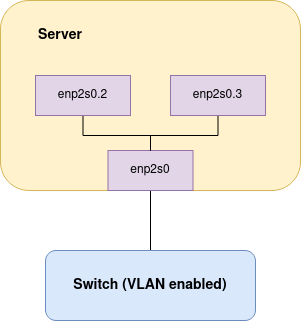
\includegraphics[width=0.4\textwidth]{img/diag_vlan.png}
			\caption{Diagrama conexión VLANs}
		\end{center}
	\end{figure}

	\pagebreak
	
	\subsection{VLAN 802.1ad: \texttt{enp2s0}.\texttt{\{0,1,2...\}.\{0,1,2...\}}}
	\noindent En este aparatado comentamos la interfaz virtual asociada al estándar 802.1ad, dicho estándar supone una actualización respecto a las VLANs basadas en 802.1q, pero añadiendo la posibilidad de tener dos tags dentro de mismo frame ethernet. En el caso del estándar 802.1q, solo podíamos tener un tag. El estándar de vlans 802.1ad es realmente útil cuando el proveedor de red y el usuario de dicha red quieren utilizar VLANs, además que amplía el límite de 4094 VLANs diferentes permitidas por el estándar 802.1Q [\ref{bib: 802.1ad}][\ref{bib: FS QinQ}]. Otra forma de la que nos podemos encontrar esta interfaz es bajo el nombre ``QinQ''. \\
	
	\noindent La estructura de la trama ethernet sigue la siguiente estructura,
	
	\begin{figure}[h]
		\begin{center}
			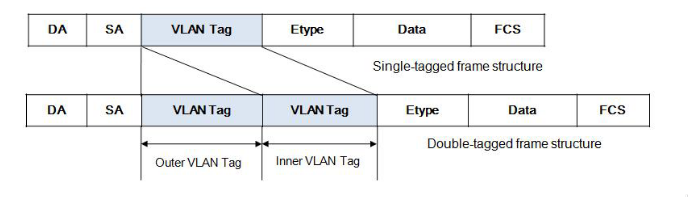
\includegraphics[width=0.8\textwidth]{img/ethernet_8021ad.png}
			\caption{Trama ethernet utilizando VLAN 802.1ad [\ref{img: frame ethernet 802.1ad}]}
			\label{ethernet 802.1ad}
		\end{center}
	\end{figure}
	
	\noindent Para configurar un enlace utilizando este estándar, tenemos que ejecutar los siguientes comandos [\ref{bib: openwrt virtual network interfaces}]:
	\begin{verbatim}
$ ip link add link eth0 eth0.1000 type vlan proto 802.1ad id 1000
$ ip link add link eth0.1000 eth0.1000.1000 type vlan proto 802.1q id 1000
 	\end{verbatim}
 
 	\noindent De esta manera, lo que hacemos es asociar una primera VLAN a una interfaz de red, utilizando 802.1ad, después a esa misma interfaz con identificador, podemos asignar otra nueva VLAN, pero esta vez utilizando el estándar 802.1q. Por lo tanto, al final nos quedaría una interfaz similar a \texttt{eth0.1000.1000} en la que podemos distinguir dos identificadores de red virtual.
	
	\pagebreak
	
	\subsection{Pares ethernet virtuales}
	\label{sec: veth}
	\noindent Los \texttt{veth} (Ethernet virtuales) son un dispositivo virtual que forman un túnel local ethernet. El dispositivo se crea en parejas. [\ref{bib:virtual interface list}]\\
	
	\noindent Los paquetes transmitidos por un extremo del ethernet virtual se reciben inmediatamente en el otro extremo. Si alguno de ellos se encuentra apagado, decimos que el link de la pareja esta también apagado. A modo de ejemplo, nos fijamos una estructura básica en la que dos aplicaciones se comunican utilizando \texttt{veth}, tal y como vemos en la figura (\ref{ej1 veth})\\
	
	\begin{figure}[h]
		\begin{center}
			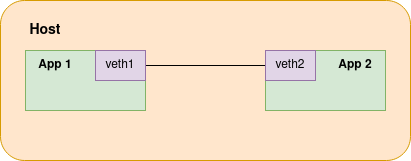
\includegraphics[width=0.5\textwidth]{img/veth_ej1.png}
			\caption{Ejemplo básico de utilización de pares virtuales ethernet}
			\label{ej1 veth}
		\end{center}
	\end{figure}

	\noindent Las interfaces virtuales ethernet se inventaron con el fin de comunicar diferentes \textit{network namespaces}. Aunque profundizaremos en ello más adelante, los \texttt{namespace} de Linux permiten encapsular recursos globales del sistema de forma aislada, evitando que puedan interferir con procesos que estén fuera del \texttt{namespace}.\\
	
	\noindent La configuración necesaria para implementar el ejemplo de la figura \ref{ej1 veth} sería el siguiente [\ref{bib:example netns veth}]:
	
	\begin{verbatim}
$ ip netns add app1
$ ip netns add app2
$ ip link add veth1 netns app1 type veth peer name veth2 netns app2
	\end{verbatim}
	
	\noindent De esta manera, tendríamos creados los \texttt{namespaces} \texttt{app1} y \texttt{app2}, que estarían interconectados entre sí. Ahora procedemos a asignar una IP a cada interfaz. 
	
	\begin{verbatim}
$ ip netns exec app1 ip addr add 10.1.1.1/24 dev veth1
$ ip netns exec app1 ip link set veth1 up
$ ip netns exec app2 ip addr add 10.1.1.2/24 dev veth2
$ ip netns exec app2 ip link set veth2 up
	\end{verbatim}
	
	\pagebreak

	\noindent Para comprobar que hay conectividad entre las diferentes aplicaciones (\texttt{app1} y \texttt{app2}) utilizamos la función del comando \texttt{ip} para ejecutar programas dentro de un \texttt{network namespace}, en este caso realizar un ping entre ambas aplicaciones:
	
	\begin{verbatim}
$ ip netns exec app1 ping 10.1.1.2
	\end{verbatim}
	
	\noindent Por otro lado, si quisiéramos una topología más compleja, como por ejemplo que varios \texttt{namespaces} puedan hacer uso de una interfaz física, tendríamos que añadir un elemento extra a nuestro sistema. El diagrama de la topología podría ser tal que así:
	
	\begin{figure}[h!]
		\begin{center}
			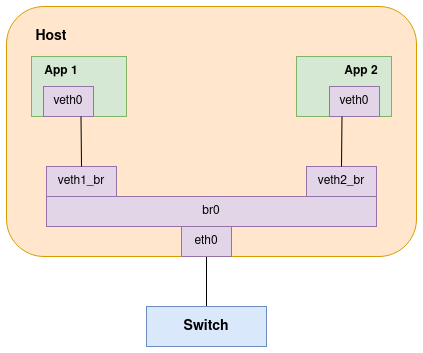
\includegraphics[width=0.5\textwidth]{img/veth_ej2.png}
			\caption{Ejemplo avanzado de utilización de pares virtuales ethernet, utilizando \texttt{bridge}}
			\label{ej2 veth}
		\end{center}
	\end{figure}
	
	\noindent Como podemos comprobar en la figura \ref{ej2 veth}, es necesario que utilicemos un ``bridge" para que podamos conectar ambas interfaces virtuales a una interfaz física, para replicar dicha topología, ejecutaremos los siguientes comandos:
	
	\begin{verbatim}
$ ip netns add app1
$ ip netns add app2
$ ip link add veth1_br type veth peer name veth0 netns app1
$ ip link add veth2_br type veth peer name veth0 netns app2

	\end{verbatim}
	
	\noindent Para definir un bridge entre las diferentes interfaces virtuales que hemos creado, utilizaremos una interfaz tipo \textit{bridge} de Linux, o bien podemos configurar dicho \textit{bridge} usando \textit{Open vSwitch}. \textit{Open vSwitch} es un programa de código abierto diseñado para ser utilizado como un switch multi-capa virtual [\ref{bib: open vswitch}][\ref{bib: veth netns ovs}].
	
	\begin{verbatim}
$ ip link add veth1_br type veth peer name veth0 netns app1
$ ip link add veth2_br type veth peer name veth0 netns app2
$ ovs-vsctl add-br ovsbr0
$ ovs-vsctl add-port ovsbr0 veth1_br
$ ovs-vsctl add-port ovsbr0 veth2_br
$ ovs-vsctl add-port ovsbr0 eth0
	\end{verbatim}

	\noindent Por último, añadimos las direcciones IP que nos faltan en la topología:
	
	\begin{verbatim}
$ ip addr add 10.1.1.10/24 dev veth1_br
$ ip link set veth1_br up
$ ip addr add 10.1.1.20/24 dev veth2_br
$ ip link set veth2_br up
$ ip netns exec app1 ip addr add 10.1.1.15/24 dev veth0
$ ip netns exec app1 ip link set veth0 up
$ ip netns exec app2 ip addr add 10.1.1.25/24 dev veth0
$ ip netns exec app2 ip link set veth0 up
$ ip netns exec app1 ip link set lo up
$ ip netns exec app2 ip link set lo up
	\end{verbatim}

	\noindent De esta manera, ya tendríamos la topología configurada con conectividad entre las diferentes aplicaciones, además de cada aplicación con una interfaz física de la máquina, todo esto utilizando una interfaz tipo \texttt{bridge}.

	\subsection{TUN/TAP}
	\noindent TUN/TAP son dos interfaces de red virtuales de Linux, que permiten dar conectividad entre programas dentro del espacio de usuario, es decir permiten conectar aplicaciones en específico con el kernel. Esta interfaz es expuesta al usuario mediante la ruta \texttt{/dev/net/tun}. Como bien hemos mencionado, existen dos tipos de interfaces virtuales controladas por \texttt{/dev/net/tun}: 
	
	\begin{itemize}
		\item TUN. Interfaces encargadas de transportar paquetes IP (trabaja sobre la capa 3).
		\item TAP. Interfaces encargadas de transportar paquetes Ethernet (trabaja sobre la capa 2).
	\end{itemize}
	
	\vspace{5px}

	\noindent \textbf{\large TUN (Capa 3)}\\
	
	\noindent Las interfaces TUN (\texttt{IFF\_TUN}) transportan paquetes PDU (\textit{Protocol Data Units}) de la capa 3 [\ref{bib: tun vs tap}]:
	\begin{itemize}
		\item En la práctica, transporta paquetes IPv4 y/o paquetes IPv6.
		\item La función \texttt{read()} devuelve un paquete de capa 3 PDU, es decir un paquete IP.
		\item Utilizando la función \texttt{write()} podemos enviar un paquete IP.
		\item No hay capa 2 en esta interfaz, por lo que los mecanismos que se ejecutan en esta capa no estarán presentes en la comunicación. Por ejemplo, no tenemos ARP.
		\item Pueden funcionar como interfaces tipo \textit{Point to Point}.
	\end{itemize}
	
	\pagebreak
	
	\noindent \textbf{\large TAP (Capa 2)}\\
	
	\noindent Las interfaces TAP (\texttt{IFF\_TAP}) transportan paquetes de capa 2 [\ref{bib: tun vs tap}]: 
	\begin{itemize}
		\item En la práctica, transporta \textit{frames Ethernet}, por lo tanto, actuaría como si fuera un adaptador virtual de Ethernet (``bridge virtual'').
		\item La función \texttt{read()} devuelve un paquete de capa L2, un \textit{frame Ethernet}.
		\item Utilizando la función \texttt{write()} permite enviar un \textit{frame Ethernet}.
		\item Podemos cambiar la MAC asociada a nuestra interfaz TAP utilizando el parámetro \texttt{SIOCSIFHWADDR}, en la función \texttt{ioctl()}, la cual usamos para crear un TUN/TAP dentro de nuestra aplicación.
	\end{itemize}

	\vspace{5px}

	% Imagen comparativa entre TUN/TAP
	\begin{figure}[h!]
		\begin{center}
			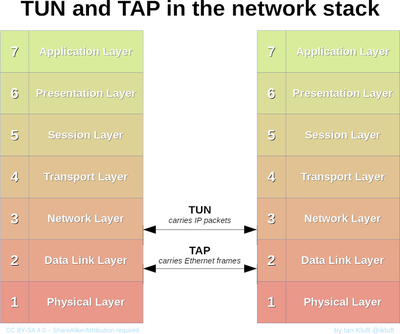
\includegraphics[width=0.6\textwidth]{img/tun_vs_tap.png}
			\caption{Comparativa en capa OSI de las interfaces TUN/TAP. [\ref{bib_img: tun tap}]}
			\label{img: tun vs tap}
		\end{center}
	\end{figure}
	
	\noindent Si nos fijamos en la figura \ref{img: tun vs tap}, podemos ver las diferencias entre ambas interfaces. Aún así, hay una que se utiliza mucho más que la otra, esta interfaz es TAP. Las interfaces tipo TAP son muy ampliamente utilizadas para realizar ``túneles virtuales'' para una aplicación en concreto. Sería la propia aplicación la encargada de monitorizar dicho ``túnel''. Podemos encontrar aplicaciones TAP en hipervisores o en clientes VPN.
	
	\pagebreak
	
	\noindent En el caso de que queramos crear interfaces TUN/TAP fuera de una aplicación, es decir, desde la línea de comandos, tendremos que utilizar los programas \texttt{tunctl} o \texttt{ip}. Para ello, podemos revisar los ejemplos \ref{lst: ej1 tunctl} y \ref{lst: ej2 tuntap ip} donde se comentan algunos de los comandos más importantes para trabajar con estar interfaces en cada uno de los programas mencionados.
	
	\vspace{10px}
	
	% Ejemplo 1: Creacion de tun/tap utilizando la linea de comandos
	\begin{lstlisting}[language=Bash, label=lst: ej1 tunctl, caption=Ejemplo de uso de \texttt{tunctl} para controlar interfaces TUN/TAP (\ref{bib: tunctl + ip})]
# Create the tap interface by default
tunctl 
# equivalent to
tunctl -p

# For users 'user' create a tap interface
tunctl -u user

# Create  Tun interface
tunctl -n
# Configure IP Address for interface and enable
ip addr add 192.168.0.254/24 dev tap0
ip link set tap0 up
# Add routing to interface
ip route add 192.168.0.1 dev tap0

# Delete interface
tunctl -d tap0
	\end{lstlisting}

	\vspace{10px}

	% Ejemplo 1.1: Creacion tun/tap pero usando comando ip
	\begin{lstlisting}[language=Bash, label=lst: ej2 tuntap ip, caption=Ejemplo de uso de \texttt{ip} para controlar interfaces TUN/TAP (\ref{bib: tunctl + ip})]
# Show help
ip tuntap help

# Create tun/tap devices
ip tuntap add dev tap0 mod tap		# create tap
ip tuntap add dev tun0 mod tun		# create tun

# Delete tun/tap devices
ip tuntap del dev tap0 mod tap		# delete tap
ip tuntap del dev tun0 mod tun		# delete tun
	\end{lstlisting}

	\pagebreak
	
	\noindent \textbf{\large Ejemplo: aplicación que crea una interfaz \texttt{tuntap}}\\

	\noindent Por otro lado, otra manera de trabajar con estas interfaces, es dejar que el programa que estemos utilizando cree dichas interfaces. Es por esto por lo que dentro del programa podemos definir que se refiera a la ruta \texttt{/dev/net/tun} para crear la interfaz necesaria. A modo de ejemplo, se implementa un programa en C que crea una interfaz TUN/TAP (en el programa elegimos cual de las dos queremos) y que devuelve el tamaño de los paquetes que reciba en dicha interfaz. Este ejemplo nos sirve para comprobar con una aplicación puede crear y gestionar una interfaz, y además, mediante un programa externo de captura de paquetes (\texttt{Wireshark}, \texttt{tcpdump}, etc...) ver los paquetes que llegan a la interfaz y cual es su estructura. \\
	
	\noindent El código utilizado sería el que vemos en [\ref{lst:tuntap.c}]. Es importante comentar que en la linea 80 podemos modificar el tipo de interfaz que vamos a crear, usaremos \texttt{IFF\_TUN} para crear un TUN y \texttt{IFF\_TAP} para crear un TAP.
	% Ejemplo: 2 Apps en C que se comunican utilizan TAP
	\vspace{10px}
	\begin{lstlisting}[language=C, label=lst:tuntap.c, caption=Aplicación de ejemplo para crear tun/tap (\texttt{tuntap.c}) (\ref{bib: code tuntap.c})]
/**
Receive incoming packages over tun/tap device. 
stdout -> size of received package
**/

#include <net/if.h>
#include <sys/ioctl.h>
#include <sys/stat.h>
#include <fcntl.h>
#include <string.h>
#include <sys/types.h>
#include <linux/if_tun.h>
#include <stdlib.h>
#include <stdio.h>

int tun_alloc(int flags)
{
	
	struct ifreq ifr;
	int fd, err;
	char *clonedev = "/dev/net/tun";
	
	if ((fd = open(clonedev, O_RDWR)) < 0) {
		return fd;
	}
	
	memset(&ifr, 0, sizeof(ifr));
	ifr.ifr_flags = flags;
	
	if ((err = ioctl(fd, TUNSETIFF, (void *) &ifr)) < 0) {
		close(fd);
		return err;
	}
	
	printf("Open tun/tap device: %s for reading...\n", ifr.ifr_name);
	
	return fd;
}

int main()
{
	
	int tun_fd, nread;
	char buffer[1500];
	
	/* Flags: IFF_TUN   - TUN device (no Ethernet headers)
	*        IFF_TAP   - TAP device
	*        IFF_NO_PI - Do not provide packet information
	*/
	tun_fd = tun_alloc(IFF_TAP | IFF_NO_PI);
	
	if (tun_fd < 0) {
		perror("Allocating interface");
		exit(1);
	}
	
	while (1) {
		nread = read(tun_fd, buffer, sizeof(buffer));
		if (nread < 0) {
			perror("Reading from interface");
			close(tun_fd);
			exit(1);
		}
		
		printf("Read %d bytes from tun/tap device\n", nread);
	}
	return 0;
}
	\end{lstlisting}

	\pagebreak

	\noindent Los pasos para realizar este ejemplo serían los siguientes:
	\begin{lstlisting}[language=Bash, label=lst: instr tuntap.c , caption=Instrucciones para realizar las pruebas con el código (\ref{lst:tuntap.c})]
# Guardamos el codigo anterior en tuntap.c
# Compilamos el programa
gcc tuntap.c -o tun

### Terminal 1
# Ejecutamos el binario, este se quedara a la escucha en la interfaz creada
./tun

### Terminal 2
# Asignamos una IP a la interfaz recien creada
ip addr add 192.168.209.138/24 dev tun0
ip link set dev tun0 up

# Capturamos el trafico que viaja por la interfaz
tcpdump -i tun0

### Terminal 3
# Mandamos trafico a la interfaz creada, un ping por ejemplo:
ping -c 4 192.168.209.139 -I tun0
	\end{lstlisting}
	
	\pagebreak
	
	%\vspace{10px}
	\noindent \textbf{\large Ejemplo: aislamiento entre puertos usando interfaz \texttt{tuntap}}\\
	
	\noindent En este ejemplo, queremos comprobar el funcionamiento de una interfaz \texttt{tap}, pero poniéndonos en el caso de que el usuario cree dicha interfaz mediante el comando \texttt{ip} y un programa externo se asocie a dicha interfaz. Para ello, vamos a utilizar la aplicación \texttt{sock} [\ref{bib: sock}], que nos servirá para crear un socket IP en un puerto específico.
	
	\begin{lstlisting}[language=Bash, caption={Compilar e instalar programa \texttt{sock} (\ref{bib: sock})}]
mkdir ~/tmp
cd tmp
tar zxvf sock-0.3.2.tar.gz
cd sock-0.3.2
./configure
make
sudo make install
	\end{lstlisting}

	\noindent Una vez tenemos el programa instalado, podemos proceder a crear la interfaz \texttt{tap}.
	
	\begin{lstlisting}[language=Bash, caption={Creación interfaz TAP}]
ip tuntap add dev tap0 mode tap
ip address add 192.168.3.1/24 dev tap0
ip link set tap0 up
ip route add 192.168.3.1 dev tap0
	\end{lstlisting}

	%\pagebreak
	
	\noindent Una vez ya tenemos creada la interfaz, podemos proceder a comprobar la funcionalidad utilizando el programa \texttt{sock}. Para ello, vamos a crear dos instancias cliente-servidor, cada una con un puerto asociado diferente.
	
	\begin{lstlisting}[language=Bash, caption={Uso de aplicacion \texttt{sock} para crear cliente servidor asociado a un puerto}]
sock -s 192.168.3.1 1025    # Terminal 1 (servidor)
sock 192.168.3.1 1025       # Terminal 2 (cliente)

sock -s 192.168.3.1 1026    # Terminal 3 (servidor)
sock 192.168.3.1 1026       # Terminal 4 (cliente)
	\end{lstlisting}

	\pagebreak

	\noindent De esta manera, podemos escribir en cada una de las terminales, y comprobar que solo son recibidas por el servidor, o cliente, asociado al puerto de la terminal en cuestión. Es decir, en las interfaces \texttt{tuntap} tenemos aislamiento entre los diferentes puertos, por lo que funcionan de manera equivalente a un enlace \texttt{ethernet} físico. En la figura (\ref{img: ejemplo sock}) podemos ver el ejemplo realizado.
	
	\begin{figure}[h!]
		\begin{center}
			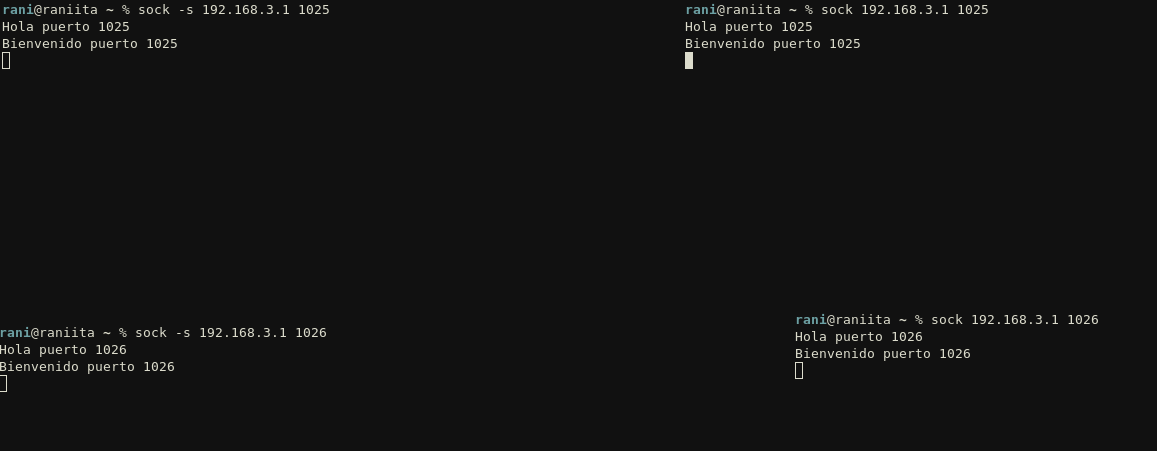
\includegraphics[width=1\textwidth]{img/ejemplo_sock.png}
			\caption{Uso de la aplicación \texttt{sock} con interfaces \texttt{tuntap}.}
			\label{img: ejemplo sock}
		\end{center}
	\end{figure}
	
	\noindent Si comprobamos la tabla de enrutamiento de la interfaz creada, \texttt{tap0}, podemos ver como aparece asociado el trafico de la IP que le dimos a dicha interfaz, con que utilice la interfaz \texttt{tap0}. (Ver figura [\ref{img: ip route tap}])
	
	\begin{figure}[h!]
		\begin{center}
			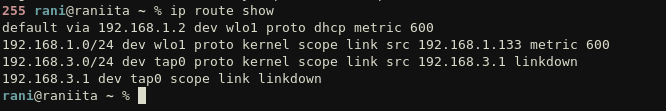
\includegraphics[width=0.75\textwidth]{img/tabla_encaminamiento_tuntap.png}
			\caption{Tabla de encamientamiento para una interfaz tuntap.}
			\label{img: ip route tap}
		\end{center}
	\end{figure}

	\pagebreak
	
	\noindent Por último, podemos comprobar la estructura de los paquetes enviados utilizando programas como \texttt{Wireshark}, \texttt{tcpdump}, etc. Es importante comentar que aunque los paquetes deberían viajar por la interfaz \texttt{tap0}, el kernel los redirige por \texttt{loopback}. En la figura \ref{img: wireshark tuntap} podemos ver un ejemplo de captura de un paquete enviado por el \texttt{tap0}.
	
	\begin{figure}[h!]
		\begin{center}
			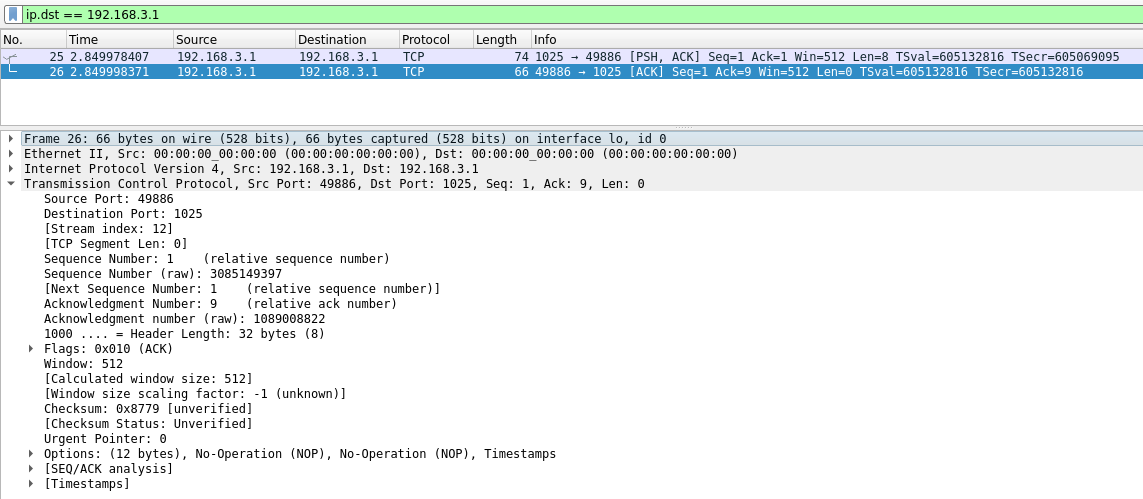
\includegraphics[width=1\textwidth]{img/wireshark_tuntap.png}
			\caption{Captura de un paquete emitido por la interfaz \texttt{tap0}.}
			\label{img: wireshark tuntap}
		\end{center}
	\end{figure}
	
	
	\pagebreak
	\section{Espacio de nombres en \textit{Linux}}
	\label{sect: espacio nombres}
	\subsection{¿Qué es un \textit{espacio de nombres}?}
	\noindent Los \textit{espacios de nombres}, o también llamados, \textit{namespaces}, son una característica del kernel de Linux que permite gestionar los recursos del kernel, pudiendo limitarlos a un proceso o grupo de procesos. Suponen una base de tecnología que aparece en las técnicas de virtualización más modernas (como puede ser Docker, Kubernetes, etc). A un nivel alto, permiten aislar procesos respecto al resto del kernel. \\
	
	\par \noindent El objetivo de cada \textit{namespaces} es adquirir una característica global del sistema como una abstracción que haga parecer a los procesos de dentro del \textit{namespace} que tienen su propia instancia aislada del recurso global.
	
	\subsection{¿Cómo crear/acceder a un \textit{namespace}?}
	\noindent Los namespaces normalmente se suelen asociar a procesos o aplicaciones en específico. Para manipular estos namespaces, podemos destacar las siguientes herramientas: 
	\begin{itemize}
		\item \texttt{unshare}. Permite asociar un namespace a un archivo. Si habia un namespace ya en ese archivo, lo sobreescribe. No nos permite reutilizar un namespace.
		\item \texttt{nsenter}. Puede acceder al namespace de un archivo existente. Podemos asociar el namespace a un archivo del sistema, de modo que aunque cerremos el proceso asociado, el archivo sigue existiendo, y por lo tanto puede ser reutilizado.
	\end{itemize}

	\noindent En resumen, si quisieramos mantener ``vivo'' un namespace, sería necesario que lo asociemos con un archivo del sistema, y después volver a ``crear'' el namespace con la herramienta \texttt{nsenter} apuntando a dicho archivo. A modo de ejemplo, sería tal que así:
	
	\begin{lstlisting}[language=Bash, label=lst: persistencia ns, caption=Ejemplo de un persistencia namespace]
touch /root/ns-uts											# Creamos un archivo
unshare --uts=/root/ns-uts /bin/bash		# Asociamos namespace UTS al archivo
hostname FooBar

# Salimos del namespace
exit

# Volvemos a entrar al namespace
nsenter --uts=/root/ns-uts /bin/bash
hostname                  # Nos devuelve 'FooBar'

# Salimos del namespace
exit

umount /root/ns-uts 			# Eliminamos el namespace definitivamente
	\end{lstlisting}
	
	\vspace{10px}
	
	\noindent Tal y como vemos en el ejemplo (\ref{lst: persistencia ns}), utilizamos los comandos \texttt{unshare} y \texttt{nsenter} para manipular un namespace de tipo UTS (hostname), veremos más en profundidad este namespace en el apartado \ref{sect: uts namespace}. Lo importante es comprobar que si asociamos un namespace a un archivo, podemos recuperar dicho namespace si utilizamos el comando \texttt{nsenter}. Además, si quisieramos eliminar permanentemente dicho namespace, tendríamos que hacer uso del comando \texttt{umount}.
	
	\subsection{¿Cúantos \textit{namespaces} hay?}
	\par\noindent El kernel ha estado en contaste evolución desde que 1991, cuando Linus Torvalds comenzó el proyecto, actualmente sigue muy activo y se siguen añadiendo nuevas características. El origen de los namespaces se remonta a la versión del kernel 2.4.19, lanzada en 2002. Conforme fueron pasando los años, más tipos diferentes de namespaces se fueron añadiendo a Linux. El concepto de \textit{User namespaces}, se consideró terminado con la versión 3.9. [\ref{bib:ns overview}]\\
	\par \noindent Actualmente, tenemos 8 tipos diferentes de namespaces, siendo el último añadido en la versión 5.8 (lanzada el 2 de Agosto de 2020). 
	
	\begin{enumerate}
		\item UTS (hostname)
		\item Mount (mnt)
		\item Process ID (pid)
		\item Network (net)
		\item User ID (user) 
		\item Interprocess Communication (ipc)
		\item Control group (cgroup)
		\item Time [\ref{bib:time ns}]
	\end{enumerate}
	
	\pagebreak
	
	\subsection{UTS namespace}
	\label{sect: uts namespace}
	\par \noindent El tipo más sencillo de todos los namespaces. La funcionalidad consiste en controlar el hostname asociado del ordenador, en este caso, del proceso o procesos asignados al namespace. Existen tres diferentes rutinas que nos permiten obtener y modifcar el hostname: 
	\begin{itemize}
		\item \textit{sethostname()}
		\item \textit{setdomainname()}
		\item \textit{uname()}
	\end{itemize}
	En una situación normal sin namespaces, se modificaría una String global, sin embargo, si estamos dentro de un namespace, los procesos asociados tienen su propia variable global asignada.\\
	
	% example uts: https://medium.com/@teddyking/linux-namespaces-850489d3ccf
	% https://www.cloudsavvyit.com/742/what-are-linux-namespaces-and-what-are-they-used-for/
	\par \noindent Un ejemplo muy basico de uso de este namespaces podría ser el siguiente [\ref{bib:ns tutorial1}]:\\
	\begin{lstlisting}[language=bash, caption=Ejemplo de uso de UTS namespace]
$ sudo su			# super user
$ hostname			# current hostname
> arch-linux					
$ unshare -u /bin/sh		# shell with UTS namespace
$ hostname new-hostname		# set hostname
$ hostname			# check hostname of the shell
> new-hostname
$ exit				# exit shell and namespace
$ hostname			# original hostname
> arch-linux
	\end{lstlisting}

	\addvspace{10px}

	\par \noindent En el ejemplo planteado, vemos que utilizamos el comando \texttt{unshare}. Utilizando la documentación de dicho comando, \texttt{man unshare}. Podemos deducir los siguiente:
	\begin{itemize}
		\item Ejecuta un programa con algunos namespaces diferentes del host.
		\item En los parametros podemos especificar cual o cuales namespaces queremos desvincular.
		\item Tenemos que especificar la ruta del ejecutable que queremos aislar
		\item La sintaxis sería tal que: \texttt{unshare [options] <program> [<argument>...]}
	\end{itemize}
	
	\pagebreak
	
	\subsection{Mount namespace}
	\noindent Este \texttt{namespace} fue el primero en aparecer en el Kernel de Linux, apareció en la versión 2.4.19, en 2002. El objetivo era restringir la visualización de la jerarquía global de archivos, dando lugar a que cada namespace tenga su propio ``set'' de puntos de montaje (directorio, archivo o enlace simbólico, que al crearse forma parte del sistema de archivos del sistema). [\ref{bib: mount namespace info 1}][\ref{bib: mount namespace info 2}] \\
	
	\noindent Una vez iniciamos el sistema, solo existe un único \texttt{mount namespace}, al que llamamos ``namespace inicial'' (\textit{default}). Los nuevos \texttt{mount namespaces} que creemos los haremos utilizando las siguientes llamadas al sistema: \texttt{clone()}, para crear un nuevo proceso asociado en el nuevo namespaces; o bien utilizando \texttt{unshare()}, para mover un proceso dentro del nuevo namespace. Cuando creamos un nuevo \texttt{mount namespace}, este recibe una copia del punto de montaje inicial, replicado por el \texttt{namespace} que lo llamada. [\ref{bib: mount namespace info 2}] \\
	
	\noindent Un concepto importante es que los \texttt{mount namespaces}, por defecto tienen activado la funcionalidad del kernel llamada \texttt{shared subtree}. Esto permite que cada punto de montaje que tengamos en nuestra máquina pueda tener su propio tipo de propagación asociado. Esta información permite que nuevos puntos de montaje en ciertas rutas se propagen a otros puntos de montaje. A modo de ejemplo, si conectamos un USB a nuestro sistema, y este se monta automáticamente en la ruta \texttt{/MI\_USB}, el contenido solo estará visible en otros \texttt{namespaces} si la propagación está configurada correctamente. [\ref{bib: mount namespace redhat}] \\
	
	%\par \noindent Un \textit{mount namespace (mnt)} supone otro tipo de espacio de nombres, en este caso relacionado con los \textit{mounts} de nuestro sistema. Lo primero es entender a que nos referimos cuando hablamos de \textit{mount}. \textit{Mount}, o montaje, hace referencia a conectar un sistema de archivos adicional que sea accesible para el sistema de archivos actual de un ordenador. Un \texttt{mount}, tiene asignado lo que se llama \textit{mount point}, que corresponde con el directorio en el que está accesible el sistema de archivo que previamente hemos montado.\\
	
	\par \noindent Por lo tanto, un namespace de tipo \textit{mount} nos permite modificar un sistema de archivos en concreto, sin que el host, o en otros namespaces, pueda ver y/o acceder a dicho sistema de archivos. Podríamos concluir que el objetivo de este espacio de nombres es el de permitir que diferentes procesos puedan tener ``vistas'' diferentes de los puntos del montaje de nuestro sistema. \\
	
	
	\noindent Un ejemplo básico de esta funcionalidad podría ser la siguiente:
	
	\addvspace{10px}
	
	\begin{lstlisting}[language=bash, caption=Uso de \texttt{mount namespace} con ``bind'']
$ sudo su		# run a shell in a new mount namespace
$ unshare -m /bin/sh
$ mount --bind /usr/bin/ /mnt/
$ ls /mnt/cp
> /mnt/cp
$ exit			# exit the shell and close namespace
$ ls /mnt/cp
> ls: cannot access '/mnt/cp': No such file or directory
	\end{lstlisting}

	\addvspace{10px}
	
	\par \noindent Como vemos en el ejemplo, dentro del namespaces lo que hacemos es crear un \textit{mount} de tipo \textit{bind}, que tiene por función que un archivo de la máquina host se monte en un directorio en específico, en este caso, un directorio unicamente del programa que hemos asignado al namespace. Otro ejemplo de uso de estos namespaces es crear un sistema de archivos temporal que solo sea visible para ese proceso.
	
	\pagebreak
	
	\noindent \textbf{\large ¿Qué es un montaje tipo \texttt{bind}?}\\
	
	\noindent Para comprender correctamente como funciona un mount namespaces, es interesante entender que es exactamente un montaje tipo \texttt{bind} y sus diferencias respecto \texttt{chroot} o \texttt{mount namespace}. [\ref{bib: what is bind}] \\
	
	\noindent En primer lugar, para trabajar respecto a montajes del sistema de archivos, utilizamos el comando de Linux \texttt{mount}. De manera primigenia, se utilizaba para ``montar'' dispositivos de almacenamiento físicos a un lugar específico del \texttt{tree} de nuestro sistema. Por ejemplo, suponemos que tenemos un disco duro conectado via interfaz \textit{SATA}. Utilizando el comando \texttt{lsblk}, determinamos que queremos montar la partición 1 del dispositivo físico con etiqueta \texttt{/dev/sda}. Por lo tanto, queremos realizar un punto de montaje de \texttt{/dev/sda1} en un lugar específico de nuestro sistema de archivos (\texttt{tree}). Para ello, podemos ejecutar el siguiente comando:
	\begin{verbatim}
$ mount /dev/sda1 /mnt/MI_USB
	\end{verbatim}

	\noindent Sin embargo, también podemos trabajar con el comando \texttt{mount} sin tener involucrados dispositivos físicos que queramos montar. Para ello, aparece el argumento \texttt{--bind} del comando \texttt{mount}, que nos permite ``vincular'' una parte del \texttt{tree} a otro emplazamiento diferente del \texttt{tree}. Esto lo podemos hacer tanto con directorios completos, como con archivos en específico.
	
	\begin{verbatim}
$ mount --bind /mnt/MI_USB /home/user/MI_USB
	\end{verbatim}

	\noindent Además, permite otras opciones interesantes. Lo primero, es que a diferencia de la herramienta \texttt{chroot}, si utilizamos \texttt{bind}, todos los puntos de montaje asociados al \texttt{tree} al que queremos aplicar el \texttt{bind} se verán también afectados, cosa que con \texttt{chroot} no sucede ya que está limitado a un único \texttt{subtree}. Por otro lado, un montaje \texttt{bind} es utilizado para aplicar una modificación sobre los permisos, o opciones del montaje, de una parte del \texttt{tree} en específico. Esto lo podemos ver con un ejemplo: queremos que ciertas carpetas de nuestra aplicación tengan permisos de solo lectura, para ello podemos ejecutar los siguientes comandos:
	
	\begin{verbatim}
$ mount --bind /mnt/MI_USB /home/user/MI_USB
$ mount -o remount,ro,bind /home/user/MI_USB
	\end{verbatim}

	\noindent Por otro lado, un tercer uso del montaje tipo \texttt{bind}, es la posibilidad realizar un montaje sobre un mismo directorio. Por ejemplo, lo realizamos sobre el directorio \texttt{/mnt/MI\_USB}:
	
	\begin{verbatim}
$ mount --bind /mnt/MI_USB /mnt/MI_USB
	\end{verbatim}

	\noindent Al ejecutar dicho comando, lo que estamos haciendo es convertir un directorio del \texttt{tree} en un \texttt{device} o dispositivo de nuestro sistema, es decir, a partir de ahora (mientras esté montado) la ruta \texttt{/mnt/MI\_USB} será tratado como un dispositivo montado sobre ese directorio. Esto mismo nos aporta cierta ventajas, ya que podemos aplicar las opciones que hemos comentado anteriormente, tales como modificar los permisos de escritura o lectura, o cambiar las opciones de montaje.

	\pagebreak

	\noindent En resumen, un montaje tipo \texttt{bind} expone una vista de un directorio (porción del \texttt{tree}) en una localización diferente. Se encarga de exponer los mismos archivos, pero con la posibilidad de diferentes opciones de montaje, diferentes ``ownership'' o permisos. Estos sistemas de archivos que muestran una vista alterada del sistema de archivos original se suelen llamar \textit{overlay filesystems}, y son comúnmente utilizados en soluciones de contenedores, algún ejemplo podría ser: \texttt{overlayfs} [\ref{bib: overlayfs}], utilizado por Docker, y que permite tener múltiples sistemas de archivos dentro de un mismo directorio (\texttt{union mounts}). \\

	\noindent Por lo tanto, una de las ventajas que nos aporta la opción \texttt{bind} es la de utilizar parte de nuestro sistema de archivos actual para destinarlo a nuestro \texttt{mount namespace}. Si bien es cierto que podemos utilizar un \texttt{mount namespace} vacío (creándolo con la herramienta \texttt{unshare}, por ejemplo), pero tendríamos que realizar un montaje dentro del namespace para cada directorio que queramos utilizar.
	
	\pagebreak
	
	\noindent \textbf{\large \texttt{tmpfs}}\\
	
	\noindent De cara al siguiente ejemplo, es interesante que repasemos la funcionalidad del kernel del linux llamada \texttt{tmpfs}. Dicha funcionalidad permite crear un sistema de archivos temporal dentro de nuestro sistema. El sistema de archivo creado reside completamente en la memoria y/o ``swap'' de nuestro sistema. Este tipo de montajes suele ser muy interesante cuando necesitamos agilizar el acceso a ciertos archivos, ya que al estar en la memoria RAM, la lectura es mucho más rápida que si lo comparamos con un disco duro e incluso un disco duro de estado solido. Sin embargo, el inconveniente que tiene es que el contenido de dicho sistema de archivos se elimina una vez reiniciemos el sistema, ya que este está almacenado en la memoria RAM de nuestro dispositivo. [\ref{bib: tmpfs arch linux}] \\
	
	\noindent Este tipo de archivos es comunmente utilizado en los siguientes directorios: \texttt{/tmp}, \texttt{/var/lock}, \texttt{/var/run}, entre otros muchos. Sin embargo, tiene una utilidad muy importante para nuestra propuesta de sistema de archivos dentro de un \texttt{mount namespace}, ya que además de poder comprobar el aislamiento entre los montajes del \texttt{mount namespace} \textit{default}, nos permite crear un montaje que puede ser heredado entre los diferentes \textit{namespaces} que creemos, aprovechando la funcionalidad de \texttt{shared tree}. \\
	
	\noindent Un ejemplo de esto podría ser el siguiente: [\ref{bib: mount namespaces containerlabs}]
	\begin{lstlisting}[language=bash, caption={Uso de \texttt{mount namespaces} con ``tmpfs''}]
# Creamos un directorio para nuestro sistema de archivos
$ mkdir /tmp/mount_ns

# Creamos el mount namespaces usando unshare
$ unshare -m /bin/bash

# Utilizamos tmpfs para crear un punto de montaje dentro del namespaces
$ mount -n -t tmpfs tmpfs /tmp/mount_ns

# Comprobamos que el montaje se ha creado correctamente
$ df -h | grep mount_ns
> tmpfs		7.8G	0	7.8G	0%	/tmp/mount_ns
$ cat /proc/mounts | grep mount_ns
> tmpfs		/tmp/mount_ns	tmpfs	rw,relatime		0	0

# En una terminal aparte (fuera del namespaces creado)
$ cat /proc/mounts | grep mount_ns
>
$ df -h | grep mount_ns
>
# Comprobamos que en el default namespace no tenemos acceso 
# al montaje tmpfs que hemos creado
	\end{lstlisting}
	
	\pagebreak
	
	\noindent \textbf{\large \texttt{shared subtrees}}\\
	
	\noindent Supongamos que un proceso quiere clonar su propio namespace, pero quiere mantener el acceso a un USB que previamente hemos montado en nuestro sistema. Para satisfacer esta situación, podemos utilizar la funcionalidad \texttt{shared subtrees}, ya que nos permite las opciones necesarias para acceder al sistema de archivos, y configurarlo específicamente para cada namespace. [\ref{bib: mount namespaces shared subtree}] \\
	
	\noindent \texttt{shared subtrees} nos aporta cuatro maneras diferentes de realizar un montaje. Dichas opciones son las siguientes:
	\begin{itemize}
		\item \textbf{\texttt{shared mount}}. Un montaje de este tipo puede ser replicado en tantos puntos de montaje y todas las réplicas seguirán siendo exactamente iguales.
		\item \textbf{\texttt{slave mount}}. Un montaje de tipo \textit{esclavo} funciona como un montaje compartido, menos para los eventos asociados al montaje y desmontaje, que solo se propagarán hacia él.
		\item \textbf{\texttt{private mount}}. Un montaje de tipo \textit{privado} no permite realizar ni recibir ningún tipo de propagación.
		\item \textbf{\texttt{unbindeable mount}}. Un montaje de tipo \textit{privado} que no permite ser asociado/vinculable.
	\end{itemize}

	\noindent Si quisiéramos asignar alguno de estos tipos de montajes a nuestro dispositivo, tendríamos que hacer uso del comando \texttt{mount} con los siguientes parámetros de estado:
	\begin{itemize}
		\item \textbf{\texttt{shared mount}} $\rightarrow$ \texttt{mount --make-shared /mnt}
		\item \textbf{\texttt{slave mount}} $\rightarrow$ \texttt{mount --make-slave /mnt}
		\item \textbf{\texttt{private mount}} $\rightarrow$ \texttt{mount --make-private /mnt}
		\item \textbf{\texttt{unbindeable mount}} $\rightarrow$ \texttt{mount --make-unbindeable /mnt}
	\end{itemize}

	\noindent Por otro lado, si quisiéramos aplicar los cambios anteriores de manera recursiva para que se cambie el tipo de montaje para todos los montajes por debajo de la jerarquía (\textit{recursivo}) del directorio que determinemos, tendríamos que utilizar los comandos siguientes: [\ref{bib: mount namespaces shared subtree 2}]
	\begin{itemize}
		\item \textbf{\texttt{shared mount}} recursivo $\rightarrow$ \texttt{mount --make-\textbf{r}shared /mnt}
		\item \textbf{\texttt{slave mount}} recursivo $\rightarrow$ \texttt{mount --make-\textbf{r}slave /mnt}
		\item \textbf{\texttt{private mount}} recursivo $\rightarrow$ \texttt{mount --make-\textbf{r}private /mnt}
		\item \textbf{\texttt{unbindeable mount}} recursivo $\rightarrow$ \texttt{mount --make-\textbf{r}unbindeable /mnt}
	\end{itemize}

	\pagebreak
	
	\noindent \textbf{\large Casos de uso de \texttt{shared subtrees}}
	
	\begin{enumerate}
		\item Supongamos un proceso que quiere crear un \texttt{namespace}, pero quiere mantener el acceso a un disco duro extraible que previamente estaba montado en el sistema. [\ref{bib: mount namespaces shared subtree}]
		
		\begin{lstlisting}[language=bash, caption={Caso de uso de \texttt{shared subtree}}]
# El administrador del sistema realiza el montaje del usb con 
# permisos de 'shared'
# mount sobre mismo directorio: modificar opciones de montaje
$ mount --bind /mnt/usb /mnt/usb
$ mount --make-shared /mnt/usb
			
# Cualquier namespace que se cree tendra acceso a /mnt/usb
# Por lo tanto, cuando un USB se conecte y se monte, dicho 
# montaje se propagara a todos los namespaces creados
		\end{lstlisting}
	
		\item Supongamos que un proceso quiere que su montaje sea invisible para otros procesos, pero que a la vez pueda ver el resto de montajes del sistema. [\ref{bib: mount namespaces shared subtree}]
		
		\begin{lstlisting}[language=bash, caption={Caso de uso de \texttt{slave mount}}]
# El administrador permite que todo el sistema sea un subtree de tipo shared
$ mount --make-rshared /
			
# Un proceso puede clonar el sistema de archivos. En un momento, 
# marca parte de sus archivos como subtree tipo slave
$ mount --make-rslave /mitreeprivado
			
# Por lo tanto, cualquier montaje realizado en /mitreeprivado no aparecera en 
# el resto de namespaces. Sin embargo, los montajes que se realicen en 
# ese directorio pero desde el namespaces default si que se progaran 
# al proceso asociado
		\end{lstlisting}
	
		\item Supongamos que queremos realizar un montaje en el que podamos ``vincular'' dos directorios, de modo que todo lo que hagamos en un directorio se refleje en el otro. [\ref{bib: mount namespaces shared subtree}]
		
		\begin{lstlisting}[language=bash, caption={Caso de uso de \texttt{bind} y \texttt{shared subtree}}]
# El administrador permite que un directorio pueda ser replicado utilizando el tipo shared
$ mount --make-shared /mnt

# Asignamos un montaje tipo bind a dicho montaje, y lo dirigimos a otro directorio
$ mount --bind /mnt /tmp

# Los montajes /mnt y /tmp se compartiran mutuamente. Cualquier montaje 
# o desmontaje que realicemos dentro de esos directorios se veran
# reflejados en el resto de montajes
		\end{lstlisting}

	\end{enumerate}

	\pagebreak
	
	\subsection{Process ID namespace}
	\par \noindent Para entender en que consiste este namespace, primero tenemos que conocer la definición de \textit{process id} dentro del Kernel. En este caso, \textit{process id} hace referencia a un número entero que utiliza el Kernel para identificar los procesos de manera unívoca. [\ref{bib:pid wikipedia}]\\
	
	\par \noindent Concretando, aísla el namespace de la ID del proceso asignado, dando lugar a que, por ejemplo, otros namespaces puedan tener el mismo PID. Esto nos lleva a la situación de que un proceso dentro de un \textit{PID namespace} piense que tiene asignado el ID "1", mientras que en la realidad (en la máquina host) tiene otro ID asignado.
	
	\addvspace{10px}
	
	\begin{lstlisting}[language=bash, caption=Uso de process id namespace]
$ echo $$		# PID de la shell
$ ls -l /proc/$$/ns	# ID espacios de nombres 
$ sudo unshare -f --mount-proc -p /bin/sh
$ echo $$		# PID de la shell dentro del ns
$ ls -l /proc/$$/ns	# nuevos ID espacio de nombres
$ ps

$ ps -ef 		# ejecutar en una shell fuera del ns. Comparar PID
$ exit
	\end{lstlisting}

	\addvspace{10px}
	
	\par \noindent Si ejecutamos el ejemplo, lo que podemos comprobar es que el ID del proceso que está dentro del namespaces (\texttt{echo \$\$}), no coincide con el proceso que podemos ver de la máquina host (\texttt{ps -ef | grep /bin/sh}). Más concretamente, el primer proceso creado en un PID namespace recibirá el pid número 1, y además de un tratamiento especial ya que supone  un \texttt{init process} dentro de ese namespace [\ref{bib:ns tutorial1}].
	
	% revisar: https://www.redhat.com/sysadmin/linux-pid-namespaces
	% https://man7.org/linux/man-pages/man7/pid_namespaces.7.html
	
	\pagebreak
	
	\subsection{Network namespace}
	\par \noindent Este namespaces nos permite aislar la parte red de una aplicación o proceso que nosotros elijamos. Con esto conseguimos que el \textit{stack} de red de la máquina host sea diferente al que tenemos en nuestro namespace. Debido a esto, el namespace crea una interfaz virtual, conjunto con el resto de necesidades para conformar un stack de red completo (tabla de enrutamiento, tabla ARP, etc...).\\
	
	\par \noindent Para crear un \textit{namespace} de tipo \textit{network}, y que este sea persistente, utilizamos la \textit{tool} ip (del \textit{package} iproute2).
	\begin{lstlisting}[language=bash, caption=Creation persistent network namespace]
$ ip netns add ns1
	\end{lstlisting}

	\par \noindent Este comando creará un network namespace llamado ns1. Cuando se crea dicho namespace, el comando ip realiza un montaje tipo bind en la ruta /var/run/netns, permitiendo que el namespace sea persistente aún sin tener un proceso asociado.
	\begin{lstlisting}[language=bash, caption=Comprobar network namespaces existentes]
$ ls /var/run/netns
or
$ ip netns
	\end{lstlisting}
	
	\addvspace{10px}

	\par \noindent Como ejemplo, podemos proceder a añadir una interfaz de \textit{loopback} al namespace que previamente hemos creado:
	\begin{lstlisting}[language=bash, caption=Asignar interfaz loopback a un namespace]
$ ip netns exec ns1 ip link dev lo up
$ ip netns exec ns1 ping 127.0.0.1
> PING 127.0.0.1 (127.0.0.1) 56(84) bytes of data. 
> 64 bytes from 127.0.0.1: icmp_seq=1 ttl=64 time=0.115 ms
	\end{lstlisting}

	\par \noindent La primera línea de este ejemplo, corresponde con la directiva que le dice al namespace que "levante" la interfaz de loopback. La segunda línea, vemos como el namespace ns1 ejecuta el ping a la interfaz de loopback (el loopback de ese namespace).
	
	\addvspace{10px}
	
	\par \noindent Es importante mencionar, que aunque existen más comandos para gestionar las redes dentro de linux (como pueden ser ifconfig, route, etc), el comando ip es el considerado sucesor de todos estos, y los anteriores mencionados, dejarán de formar parte de Linux en versiones posteriores. Un detalle a tener en cuenta con el comando ip, es que es necesario tener privilegios de administrador para poder usarlo, por lo que deberemos ser root o utilizar sudo.
	
	\addvspace{10px}
	
	\par \noindent Por lo tanto, utilizando el comando ip, podemos recapitular que si utilizamos la siguiente directiva, podemos ejecutar el comando que nosotros indiquemos, pero dentro del network namespace que previamente hemos creado.
	\begin{lstlisting}[language=bash, caption=Ejecutar cualquier programa con un network namespace]
$ ip netns exec <network-namespace> <command>
	\end{lstlisting}

	\pagebreak
	
	\noindent \textbf{\large Ejemplo: topología de red usando \texttt{network namespaces} y NAT}\\
	\par \noindent Una de las problemáticas que supone el uso de los network namespaces, es que solo podemos asignar \textbf{una interfaz real} a \textbf{un namespace}. Suponiendo el caso en el que el usuario root tenga asignada la interfaz eth0 (identificador de una interfaz de red física), significaría que solo los programas en el namespace de root podrán acceder a dicha interfaz. En el caso de que eth0 sea la salida a Internet de nuestro sistema, pues eso conllevaría que no podríamos tener conexión a Internet en nuestros namespaces. La solución para esto reside en los \textbf{veth-pair}.
	
	\addvspace{10px}
	
	\par \noindent Un veth-pair funciona como si fuera un cable físico, es decir, interconecta dos dispositivos, en este caso, interfaces virtuales. Consiste en dos interfaces virtuales, una de ellas asignada al root namespace, y la otra asignada a otro network namespace diferente. Si a esta arquitectura le añadimos una configuración de IP válida y activamos la opción de hacer NAT en el eth0 del host, podemos dar conectividad de Internet al network namespace que hayamos conectado.
	
	\addvspace{10px}
	
	\begin{lstlisting}[language=bash, caption=Ejemplo configuración de NAT entre eth0 y veth]
# Remove namespace if exists
$ ip netns del ns1 &>/dev/null

# Create namespace
$ ip netns add ns1

# Create veth link
$ ip link add v-eth1 type veth peer name v-peer1

# Add peer-1 to namespace.
$ ip link set v-peer1 netns ns1

# Setup IP address of v-eth1
$ ip addr add 10.200.1.1/24 dev v-eth1
$ ip link set v-eth1 up

# Setup IP address of v-peer1
$ ip netns exec ns1 ip addr add 10.200.1.2/24 dev v-peer1
$ ip netns exec ns1 ip link set v-peer1 up
# Enabling loopback inside ns1
$ ip netns exec ns1 ip link set lo up

# All traffic leaving ns1 go through v-eth1
$ ip netns exec ns1 ip route add default via 10.200.1.1
	\end{lstlisting}

	%\addvspace{10px}
	
	\pagebreak

	\par \noindent Siguiendo el ejemplo propuesto, llegamos hasta el punto en el que el tráfico saliente del namespace ns1, será redirigido a v-eth1. Sin embargo, esto no es suficiente para tener conexión a Internet. Tenemos que configurar el NAT en el eth0.
	
	\begin{lstlisting}[language=bash, caption=Configuración de NAT para dar Internet a un network namespace]
# Share internet access between host and NS

# Enable IP-forwarding
$ echo 1 > /proc/sys/net/ipv4/ip_forward

# Flush forward rules, policy DROP by default
$ iptables -P FORWARD DROP
$ iptables -F FORWARD

# Flush nat rules.
$ iptables -t nat -F

# Enable masquerading of 10.200.1.0 (ip of namespaces)
$ iptables -t nat -A POSTROUTING -s 10.200.1.0/255.255.255.0 -o eth0 
	-j MASQUERADE

# Allow forwarding between eth0 and v-eth1
$ iptables -A FORWARD -i eth0 -o v-eth1 -j ACCEPT
$ iptables -A FORWARD -o eth0 -i v-eth1 -j ACCEPT
	\end{lstlisting}
	
	\addvspace{10px}
	
	\par \noindent Si todo lo hemos configurado correctamente, ahora podríamos realizar un ping hacia Internet, y este nos debería resultar satisfactorio.
	\begin{verbatim}
$ ip netns exec ns1 ping google.es
> PING 8.8.8.8 (8.8.8.8) 56(84) bytes of data.
> 64 bytes from 8.8.8.8: icmp_seq=1 ttl=50 time=48.5ms
> 64 bytes from 8.8.8.8: icmp_seq=2 ttl=50 time=58.5ms
	\end{verbatim}

	\addvspace{10px}
	
	\par \noindent Aún así, no resulta muy cómodo el utilizar \texttt{ip netns exec} seguido de la aplicación a utilizar. Es por esto por lo que es común ejecutar dicho comando para asignar el network namespace a una shell. Esto sería tal que así:
	\begin{verbatim}
$ ip netns exec ns1 /bin/bash
	\end{verbatim}
	\par \noindent Utilizaremos \texttt{exit} para salir de la shell y abandonar el network namespace.


	% https://blogs.igalia.com/dpino/2016/04/10/network-namespaces/
	
	\pagebreak
	\subsection{User ID namespace}
	\par \noindent Cada sistema dispone de una manera de monitorizar que usuario es el dueño de cada archivo. Esto permite al sistema restringir el acceso a aquellos archivos que consideramos sensibles. Además, bloquea el acceso entre diferentes usuarios dentro del mismo sistema. Para el usuario, este identificador de usuarios se muestra como el usuario que en ese momento está conectado, sin embargo, para nuestro sistema, el identificador de usuario esta compuesto por una combinación arbitraria de caracteres alfanuméricos. Con el fin de mantener el monitoreo correctamente, hay un proceso encargado de transformar esos caracteres a un número específico de identificación (UID), como por ejemplo sería 1000. Es este valor el que se asocia con los archivos creados por este usuario. Esto nos aporta la ventaja de que, si un usuario cambia su nombre, no es necesario reconstruir el sistema de archivos, ya que su UID sigue siendo 1000.\\
	
	\par \noindent Si por ejemplo queremos ver el UID del usuario que estamos usando en este momento, podemos ejecutar: \textit{echo \$UID}, el cual nos devolverá el número asociado a nuestro usuario, en mi caso es el 1000.\\
	
	\par \noindent Además de diferenciar entre los IDs de usuarios (UID), también se nos permite separar entre IDs de grupos (GID). En linux, un grupo sirve para agrupar usuarios de modo que un grupo puede tener asociado un privilegio que le permite usar un recurso o programas.\\
	
	\par \noindent Por lo tanto, el namespace de UID, lo que nos permite es tener un UID y GID diferente al del host. 
	
	\begin{lstlisting}[language=bash, caption=Ejemplo de uso UID namespace]
$ ls -l /proc/$$/ns		# espacios de nombres originales
$ id
> uid=1000(user) gid=1000(user) groups=1000(user), ...
$ unshare -r -u bash	# Crea un namespace de tipo usuario, programa bash
$ id
> uid=0(root) gid=0(root) groups=0(root),65534(nobody)
$ cat /proc/$$/uid_map
>          0       1000          1
$ cat /etc/shadow		# No nos deja acceder
> cat: /etc/shadow: Permission denied
$ exit
	\end{lstlisting}
	
	\addvspace{20px}
	
	\par \noindent Como vemos en el ejemplo, el UID de usuario difiere de la máquina host. Dentro del namespace, tenemos UID 0, sin embargo, eso no significa que podamos acceder a los archivos con UID 0 de la máquina host, ya que en verdad lo que hace el namespace es \textit{mapear} el UID 1000 al 0. [\ref{bib:ns tutorial1}]
	
	%\pagebreak
	
	\subsection{Interprocess Communication namespace (IPC)}
	\par \noindent Este namespace supone uno de los más técnicos, complicados de entender y explicar. IPC (Interprocess comunication) controla la comunicación entre procesos, utilizando zonas de la memoría que están compartidas, colas de mensajes, y semáforos. La aplicación más común para este tipo de gestión es el uso en bases de datos.
	
	\pagebreak
	
	\subsection{Control group namespace}
	\par \noindent Los grupos de control, o \texttt{cgroups}, de Linux suponen un mecanismo para controlar los diferentes recursos de nuestro sistema. Cuando un \texttt{cgroup} está activo, puede controlar la cantidad de CPU, RAM, acceso I/O, o cualquier faceta que un proceso puede consumir. Además, permiten definir jerarquías en las que se agrupan, de manera en la que el administrador del sistema puede definir como se asignan los recursos o llevar la contabilidad de los mismos. Cgroups permite las siguientes funcionalidades [\ref{bib: cgroups}]: 
	\begin{itemize}
		\item \textbf{Limitar recursos}. Podemos configurar un grupo para limitar un recurso (o varios de ellos) para cada proceso que asignemos.
		\item \textbf{Priorizar tareas}. Podemos controlar cuantos recursos utiliza un proceso, comparándolo con otro proceso en un grupo diferente.
		\item \textbf{Monitorización}. Los límites establecidos para los recursos son monitorizados y son reportados al usuario.
		\item \textbf{Control}. Podemos controlar el estado de los procesos asociados a un grupo con un solo comando, pudiendo elegir entre ``congelado'', ``parado'' o ``reiniciado''.
	\end{itemize}
	
	\noindent La primera versión de \texttt{cgroups} aparece en el Kernel en 2007, siendo esta la versión más estandarizada por la mayoría de distribuciones. Sin embargo, en 2016 aparece \texttt{cgroups v2} en el Kernel, aportando mejoras en la simplificación de los arboles de jerarquías de la ruta \texttt{/sys/fs/cgroup}, además de nuevas interfaces, aportando las bases para contenedores que utilizan el concepto de ``\textit{rootless}''. \\
	
	\par \noindent En el caso de la versión \texttt{v1}, los \texttt{cgroups} se crean en el sistema de archivos virtual en la ruta \texttt{/sys/fs/cgroup}. Para crear un nuevo grupo, en nuestro caso con el objetivo de limitar un proceso en memoria, tendríamos que ejecutar lo siguiente:
	\begin{verbatim}
$ mkdir /sys/fs/cgroup/memory/<NombreGrupo>
	\end{verbatim}

	\noindent De esta manera, ya tendríamos un nuevo grupo creado, asociado al \texttt{cgroup} de memory. Si ejecutamos el comando ls en el directorio que acabamos de crear, podemos comprobar como se han generado una serie de recursos: 
	
	\begin{figure}[h!]
		\begin{center}
			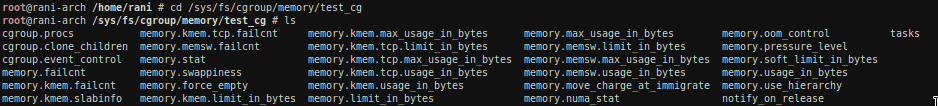
\includegraphics[width=1\textwidth]{img/cgroup_memory_ls.png}
			\caption{Archivos asociados al grupo \texttt{test\_cg} una vez lo creamos}
		\end{center}
	\end{figure}

	\pagebreak
	
	\noindent \textbf{\large Ejemplo: limitar uso de memoria RAM}\\
	
	\noindent Si quisiéramos establecer un límite en el uso de memoria, tendríamos que escribir en el archivo \texttt{memory.limit\_in\_bytes}, a modo de ejemplo, establecemos un límite de 50MB. Esto se haría tal que:
	\begin{verbatim}
$ echo 50000000 > /sys/fs/cgroup/memory/<NombreGrupo>/memory.limit_in_bytes
	\end{verbatim}

	\noindent Para comprobar el funcionamiento de este límite de memoria, vamos a asociarle un programa escrito en Python que consume mucha memoria RAM de golpe. El programa en cuestión vendría dado por el siguiente código:
	\begin{lstlisting}[language=Python, caption={Programa en Python que consume 4 GB de RAM}]
#!/usr/bin/python
import numpy

print("cgroup testing program (memory limit)")
result = [numpy.random.bytes(1024*1024) for x in range(1024*4)]
print("RAM used: {}M".format(len(result)))
	\end{lstlisting}

	\noindent Ejecutamos el programa, y comprobamos como la salida por consola es tal que: 
	
	\begin{figure}[h!]
		\begin{center}
			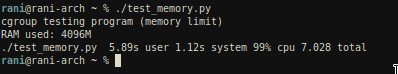
\includegraphics[width=0.6\textwidth]{img/cgroup_python1.png}
			\caption{Salida tras ejecutar el programa de Python sin limitar}
			\label{img: cgroup python 1}
		\end{center}
	\end{figure}

	\noindent Sin embargo, ahora vamos a proceder a limitar ese mismo programa en memoria. Para ello, vamos a añadir el PID asociado a la ejecución de dicho programa al siguiente archivo (ejecutando el script \texttt{./test\_memory.py \&}, nos aparece el PID):
	\begin{verbatim}
$ echo 62482 > /sys/fs/cgroup/memory/<NombreGrupo>/cgroup.procs
	\end{verbatim}
	
	\noindent De esta manera ya estaríamos limitando la memoria de ese programa en concreto. Al limitarlo, podemos comprobar como la salida en consola es tal que: 
	
	\begin{figure}[h!]
		\begin{center}
			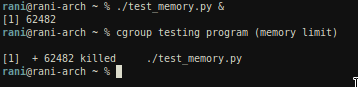
\includegraphics[width=0.6\textwidth]{img/cgroup_python2.png}
			\caption{Salida tras ejecutar el programa de Python, una vez limitado}
			\label{img: cgroup python 2}
		\end{center}
	\end{figure}

	\pagebreak
	
	\noindent Como podemos comprobar en las imágenes [\ref{img: cgroup python 1}] y [\ref{img: cgroup python 2}], la salida del programa no coincide. Esto es debido a que como el programa Python ha superado el límite establecido para su grupo, \texttt{cgroups} cerrado bruscamente dicho programa, por lo tanto no nos aparece la memoria consumida por el programa, solo se nos notifica que el proceso con PID 62482 ha pasado a estado ``\textit{killed}''. \\
	
	\vspace{10px}
	\noindent \textbf{\large Ejemplo: limitar uso de CPU}\\
	
	\noindent Por otro lado, si quisiéramos limitar el uso de CPU de un programa, tendríamos que escribir en los archivos \texttt{cpu.cfs\_quota\_us} o \texttt{cpu.cfs\_period\_us}, dentro de la rama de \texttt{cpu}. Estos parámetros hacen referencia al tiempo de ejecución asociado a un proceso. En este ejemplo, vamos a limitar el proceso a 1 ms (1000 us), esto sería tal que:
	
	\begin{verbatim}
$ echo 1000 > /sys/fs/cgroup/cpu/<NombreGrupo>/cpu.cfs_quota_us
	\end{verbatim}

	\noindent Esto significa que cada 100ms de tiempo, el proceso está limitado por cgroups a utilizar solo 1ms del tiempo de CPU, dando lugar a utilizar solo el 1\% de la CPU. \\

	\noindent Para comprobar el funcionamiento, podemos utilizar el siguiente \textit{script} en \textit{background} que nos pone un núcleo de la CPU al 100\%:
	\begin{verbatim}
$ while : ; do : ; done &
	\end{verbatim}

	\noindent Al ejecutar dicho comando, la tarea se quedará funcionando en \textit{background}. Podemos comprobarlo si utilizamos herramientas para ver el consumo de los procesos, como pueden ser \texttt{top} o \texttt{htop}. Una vez tenemos el PID asociado a la tarea de prueba, podemos proceder a añadirlo a los procesos que son limitados con el cgroup creado, en este caso únicamente para limitar la CPU.
	\begin{verbatim}
$ echo <PID> > /sys/fs/cgroup/cpu/<NombreGrupo>/tasks
	\end{verbatim}

	\noindent Una vez ejecutado, si volvemos a ejecutar \texttt{top} o \texttt{htop}, podemos ver como el tiempo asignado al recurso será mucho mejor, y estrictamente igual o inferior al límite que establecimos en la creación de la regla para nuestro cgroup.	\\
	
	\vspace{10px}
	\noindent \textbf{\large Ejemplo: monitorización de un recurso}\\
	
	\noindent A modo de comentario, otra de las tareas importante que desempeña cgroups es la monitorización del consumo de recursos de ciertas aplicaciones. Por ejemplo, para el caso del \textit{runtime} de Docker (hablaremos más en profundidad en [\ref{sec: docker}]) para ejecutar contenedores basados en namespaces, utiliza cgroups para concretar el consumo (CPU, RAM, uso de disco, red...) que tiene un contenedor en concreto. De este modo, podemos discernir y aplicar limitaciones a un contenedor en específico, sin tener que afectar a otros contenedores que estén funcionando en ese momento en el host. \\
	
	\noindent Para estas tareas, limitación y monitorización de recursos en contenedores de Docker, este nos facilita una serie de comandos para facilitar la creación y asignación de contenedores a un cgroup en específico, facilitando en consecuencia el uso de cgroups para limitar los recursos de los contenedores que estemos utilizando.
	
	%\addvspace{60px}
	
	\pagebreak
	
	\subsection{Time namespace}
	\par \noindent Por último, nos queda el namespaces asociado al tiempo. Este namespace fue propuesto para que se incorporara al kernel de Linux en 2018 y en enero de 2020 fue añadido a la versión mainline de Linux. Apareció en la release 5.6 del kernel de Linux. \\
	
	\par \noindent El namespace time, permite que por cada namespace que tengamos, podamos crear desfases entre los relojes monotónicos (CLOCK\_MONOTONIC) y de boot (CLOCK\_BOOTTIME), de la máquina host. Esto permite que dentro de los contendores se nos permita cambiar la fecha y la hora, sin tener que modificar la hora del sistema host. Además, supone una capa más de seguridad, ya que no estamos vinculando directamente la hora a los relojes físicos de nuestro sistema. [\ref{bib:time ns kernel}]\\
	
	\par \noindent Un namespace de tipo time, es muy similar al namespace de tipo PID en la manera de como lo creamos. Utilizamos el comando unshare -T, y mediante una systemcall se nos creará un nuevo time namespace, pero no lo asocia directamente con el proceso. Tenemos que utilizar setns para asociar un proceso a un namespace, además todos los procesos dependientes también tendrán asignado dicho namespace. 
	
	%\addvspace{80px}
	\vspace{80px}
	
	\begin{figure}[h!]
		\begin{center}
			% https://8gwifi.org/docs/linux-namespace.jsp
			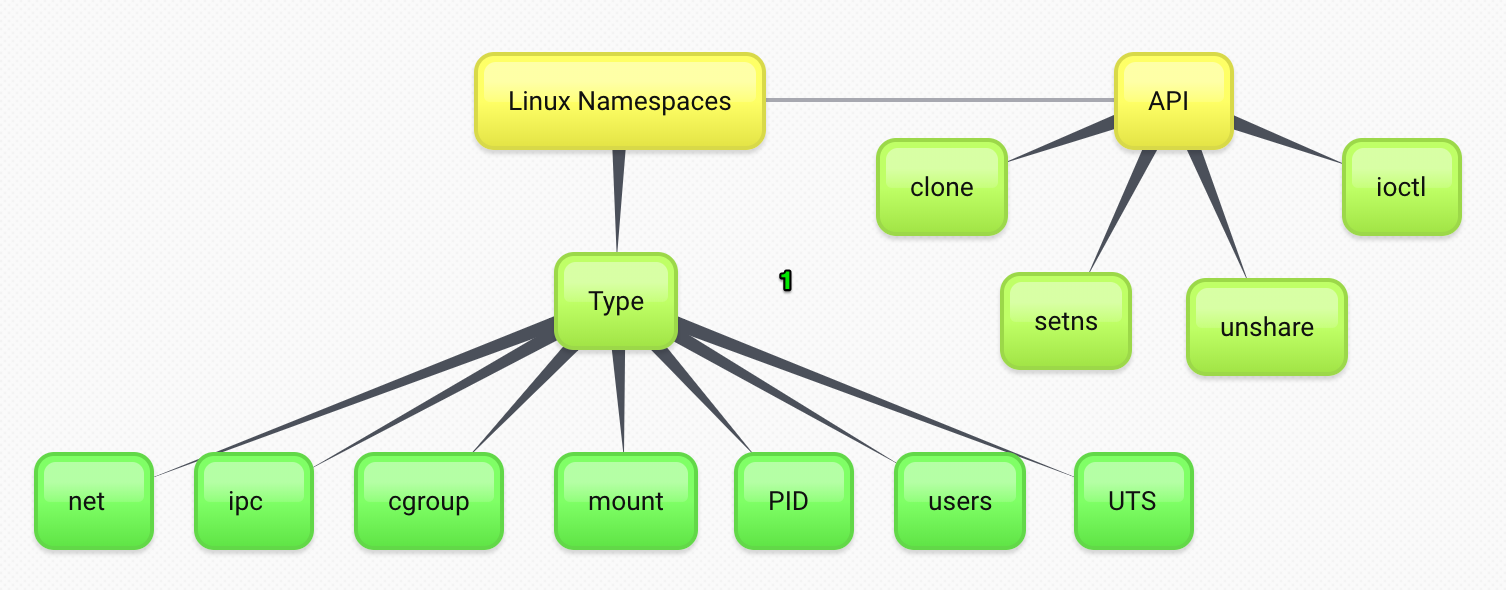
\includegraphics[width=1\textwidth]{img/linux-namespace1.png}
			\caption{Diferentes namespaces en Linux y su API de acceso. (\ref{bib:img1})}
		\end{center}
	\end{figure}
	
	%\begin{figure}[h]
	%	\begin{center}
	%		% https://twitter.com/b0rk/status/1240364585766576128/photo/1
	%		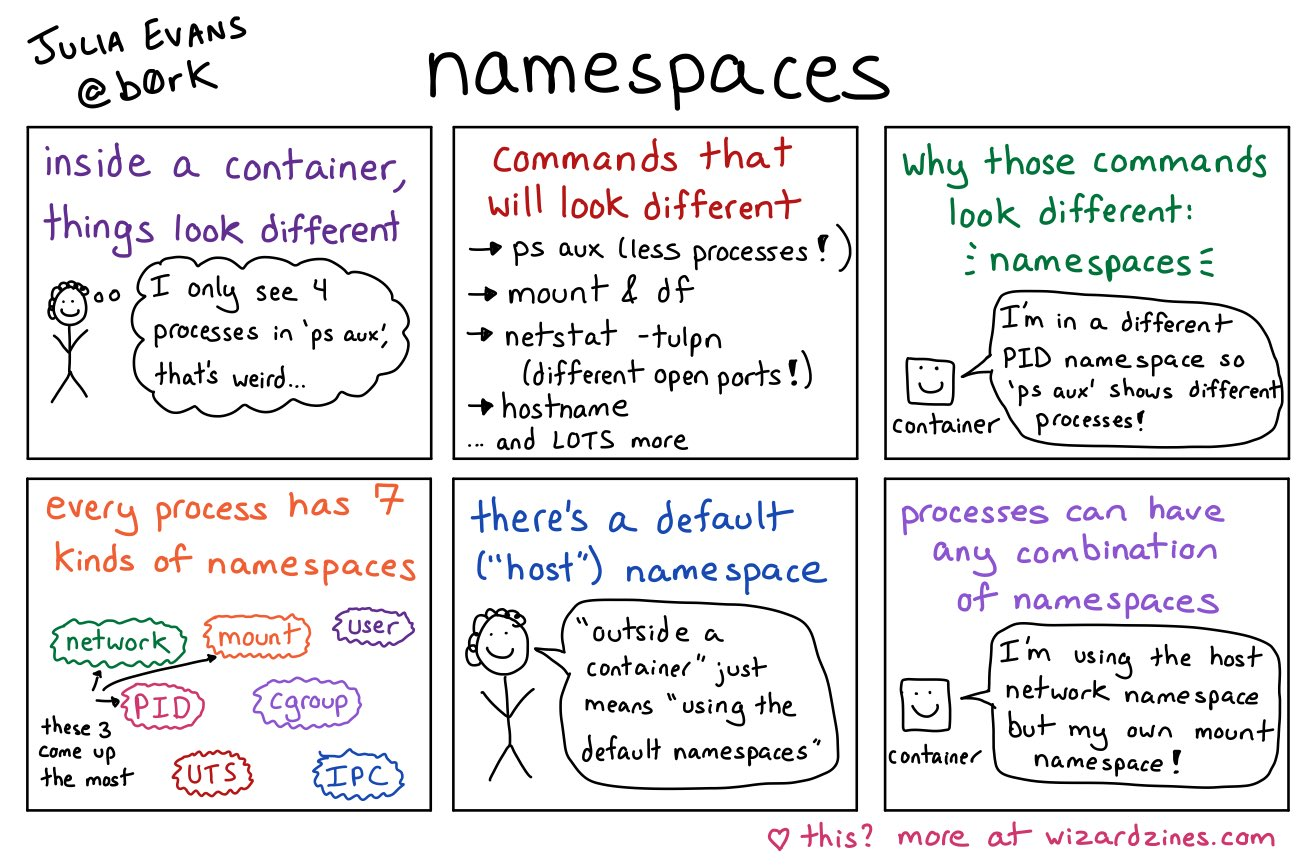
\includegraphics[width=0.8\textwidth]{img/how_containers_work.jpg}
	%		\caption{Como funcionan los contenedores. (\ref{bib:img2})}
	%	\end{center}
	%\end{figure}
	
	\pagebreak
	
	\subsection{Ejemplo: topología de red usando comando \texttt{ip}}
	\noindent En este apartado, vamos a detallar un ejemplo de como funciona el comando IP manejando los 'network namespaces'.\\
	
	\noindent Creamos los \textit{network namespaces}, en este caso, con nombre h1 y h2. El sistema no crea directamente el namespace, lo que en realidad hace es definirlos en el sistema. El \textit{network namespace} se crea cuando una aplicación se asocia a el.
	\begin{verbatim}
$ ip netns add h1
$ ip netns add h2
	\end{verbatim}

	\noindent Si utilizamos el comando \texttt{ip netns}, nos mostrará los network namespaces existentes. Como es un sub-comando de \texttt{ip}, muestra los ns que el comando \texttt{lsns} no muestra. \\
	
	\noindent Procedemos a asociar una aplicación a cada netns. Utilizamos \texttt{bash}.
	\begin{verbatim}
$ ip netns exec h1 bash
$ ip netns exec h2 bash
	\end{verbatim}

	\noindent Ahora, si que podemos utilizar el comando \texttt{lsns}. Comprobamos que si nos aparecen los ns que hemos creado, cosa que antes de asociar una aplicación al ns, no pasaba. \\
	
	\noindent El comando \texttt{ip} crea automaticamente un \textit{nsfs} para poder colocar los archivos de configuración del \textit{netns}. Para ello, debe crearse el directorio \texttt{/etc/netns/h1} y poner en el los archivos de configuración de la red.
	\begin{verbatim}
$ mkdir /etc/netns/h1
$ echo "nameserver 8.8.8.8" > /etc/netns/h1/resolv.conf
	\end{verbatim}

	\noindent En este momento, tenemos el ns configurado con DNS. Nos quedaría realizar la conexión entre el ethernet físico de nuestro \textit{host} y las interfaces de nuestros namespaces. Para ello, vamos a utilizar un conmutador virtual, en este caso Open vSwitch.
	\begin{verbatim}
$ systemctl enable --now openvswitch.service
	\end{verbatim}

	\noindent Creamos un \textit{brige} utilizando el OpenvSwitch.
	\begin{verbatim}
$ $ ovs-vsctl add-br s1
	\end{verbatim}

	\noindent Utilizando el comando \texttt{ip}, creamos las interfaces virtuales de ethernet y las asignamos a sus namespaces.
	\begin{verbatim}
$ ip link add h1-eth0 type veth peer name s1-eth1
$ ip link add h2-eth0 type veth peer name s1-eth2
$ ip link set h1-eth0 netns h1
$ ip link set h2-eth0 netns h2
	\end{verbatim}

	\pagebreak
	
	\noindent Utilizando el comando \texttt{ovs-vsctl}, asignamos al \textit{bridge} el otro par ethernet que hemos creado para cada namespace.
	\begin{verbatim}
$ ovs-vsctl add-port s1 s1-eth1
$ ovs-vsctl add-port s1 s1-eth2
	\end{verbatim}

	\noindent Verificamos que el controlador sea \textit{standalone}, así el switch se comportará como un \textit{learning-switch}.
	\begin{verbatim}
$ ovs-vsctl set-fail-mode br0 standalone
	\end{verbatim}

	\noindent Como la conexión es desde localhost al exterior, entendemos que es una conexión fuera de banda.
	\begin{verbatim}
$ ovs-vsctl set controller br0 connection-mode=out-of-band
	\end{verbatim}

	\noindent En este momento, tenemos todos configurado a falta de habilitar las diferentes interfaces de nuestra topología.
	\begin{verbatim}
$ ip netns exec h1 ip link set h1-eth0 up
$ ip netns exec h1 ip link set lo up
$ ip netns exec h1 ip add add 10.0.0.1/24 dev h1-eth0
$ ip netns exec h2 ip link set h2-eth0 up
$ ip netns exec h2 ip link set lo up
$ ip netns exec h2 ip add add 10.0.0.2/24 dev h2-eth0
$ ip link set s1-eth1 up
$ ip link set s1-eth2 up
	\end{verbatim}

	\noindent Ahora tenemos todas las interfaces configuradas, el switch activado y el sistema interconectado, por lo que podemos ejecutar un ping en una de las terminales de los namespaces para verificar la topología.
	\begin{verbatim}
$ ip netns exec h1 ping -c4 10.0.0.2
	\end{verbatim}

	\noindent Si queremos revertir todas las configuraciones que hemos hecho, lo que tenemos que hacer es ejecutar los siguientes comandos:
	\begin{verbatim}
$ ovs-vsctl del-br s1
$ ip link delete s1-eth1
$ ip link delete s1-eth2
$ ip netns del h1
$ ip netns del h2
	\end{verbatim}

	\pagebreak

	\subsection{Ejemplo: topología de red usando comando \texttt{unshare}}
	\noindent En el ejemplo anterior, utilizábamos el comando \texttt{ip} para manejar los network namespaces, sin embargo, eso nos limitaba los tipos namespaces que queríamos asignar a nuestro namespace. En contra partida a esto, el comando \texttt{unshare} nos da más libertad a la hora de crear los namespaces. \\
	
	\noindent Utilizando \texttt{unshare}, no podemos ponerle un nombre, pero sí que nos permite asociarlo a un archivo, que montará con tipo \textit{bind}. Esto nos permitirá utilizar en namespace aunque no haya ningún proceso corriendo en el, para ello podemos utilizar el comando \texttt{nsenter}.
	\begin{verbatim}
$ touch /var/net-h1
$ touch /var/uts-h1
$ unshare --net=/var/net-h1 --uts=/var/uts-h1 /bin/bash
	\end{verbatim}

	\noindent Utilizando el comando \texttt{nsenter} podemos ejecutar comandos dentro del namespace.
	\begin{verbatim}
$ nsenter --net=/var/net-h1 --uts=/var/uts-h1 hostname h1
$ nsenter --net=/var/net-h1 --uts=/var/uts-h1 ip address
	\end{verbatim}

	\noindent Para destruir el namespace, lo que tendremos que hacer es desmontar los archivos asignados a dicho namespace.
	\begin{verbatim}
$ umount /var/net-h1
$ umount /var/uts-h1
	\end{verbatim}

	\noindent Como será común necesitar más de un namespace, en la mayoría de los casos tendremos que utilizar los comandos \texttt{unshare} y \texttt{nsenter}.

	\pagebreak
	
	\section{Virtualización ligera y contenedores}
	\label{sec: virt ligera y contenedores}
	
	\noindent En este capítulo vamos a trabajar el concepto de virtualización ligera, que ya introdujimos en el apartado \ref{sect: virt ligera}, pero esta vez aplicando los conceptos de \texttt{namespaces} del apartado anterior. Además, presentaremos el concepto de \textit{contenedor}, y como supone una de las piezas más importantes para la virtualización tal y como hoy día la conocemos. \\
	
	\noindent Recuperando la definición de \textbf{virtualización ligera}, entendemos este tipo de virtualización como aquella que \textbf{se realiza a nivel de sistema operativo}, permitiendo la coexistencia de diferentes espacios aislados entre sí. En dichos espacios, podremos ejecutar de manera aislada nuestras aplicaciones. Como punto en común, todos los espacios aislados que creemos, \textbf{utilizarán} como base \textbf{el mismo \texttt{kernel}}. La tecnología clave para realizar esta virtualización serán los diferentes \texttt{namespaces}, comentados en el apartado \ref{sect: espacio nombres}, que podremos combinar a nuestro gusto con el fin de crear un espacio aislado con todos los recursos necesarios para satisfacer las necesidades de nuestra aplicación. \\
	
	\noindent La principal ventaja que encontramos al utilizar \texttt{namespaces}, respecto a otro tipo de virtualizaciones como podrían ser las máquinas virtuales, es el aprovechamiento de los recursos de la máquina host. Al tener todos el mismo kernel, evitamos tener por duplicados los kernels para cada una de las instancias a realizar, ahorrando ciclos de CPU, como espacio en RAM.\\
	
	\noindent Por otro lado, tenemos el concepto de \textbf{contenedor}. Entendemos contenedor, en el ambito de la virtualización, como una abstracción a alto nivel de un sistema aislado creado utilizando \texttt{namespaces} y \texttt{cgroups}. Por lo tanto, si el kernel nos da la posibilidad de trabajar a bajo nivel utilizando dichos \texttt{namespaces}, en este caso, buscamos ir más allá y encapsular dicho espacio aislado en unas APIs de alto nivel, que sean mucho más fáciles de entender y de implementar. Tenemos muchos ejemplos de sistemas que trabajan con contenedores, y muchos de ellos implementados en una amplia variedad de lenguajes [\ref{bib:container is a lie}]. Algunos de los más importantes son:
	\begin{itemize}
		\item \texttt{LXC}, LinuX Containers, escrito en C: \url{https://linuxcontainers.org/}
		\item \texttt{Docker}, escrito en Go: \url{https://www.docker.com/}
		\item \texttt{Podman}, escrito en Go: \url{https://podman.io/}
		\item \texttt{systemd-nspawn}, escrito en C, implementado dentro de \texttt{systemd}: \url{https://github.com/systemd/systemd}
		\item \texttt{Vagga}, escrito en Rust: \url{https://github.com/tailhook/vagga}
	\end{itemize}

	\noindent Por último, es interesante comentar el concepto de \texttt{chroot}, ya que muchas de estas abstracciones de los \texttt{namespaces} hacen uso de esta técnica para su funcionamiento. Un \texttt{chroot} es una operación Unix que permite cambiar la ruta aparente de un directorio para un usuario en específico. Un proceso ejecutado después de realizar un \texttt{chroot} solo tendrá acceso al nuevo directorio definido y a sus subdirectorios, esta operación recibe el nombre de \texttt{chroot jail}, ya que los procesos no pueden leer ni escribir fuera del nuevo directorio. Este método suele ser de gran utilidad en virtualizaciones a nivel de kernel, es decir, virtualización ligera o contenedores. [\ref{bib: chroot jail}]
	
	\pagebreak
	
	\subsection{Creando nuestro propio ``contenedor''}
	%% TODO
	\noindent En este apartado vamos a comentar las diferentes fases que deberíamos seguir si quisiéramos implementar nuestro propio contenedor. En este caso, las fases son muy similares a las que utiliza la tecnología de Docker, la cual comentaremos más en detalle en los apartados siguientes. \\
	
	\noindent Lo primero, es interesante comentar que aunque nos referimos a contenedores, muchas personas entienden contenedores como únicamente los \texttt{Docker Containers}, sin embargo existen otros \texttt{runtimes} para ejecutar contenedores en el host. En general, todos implementan las especificaciones realizadas por \textit{Linux Foundation's Container Initiative} (\texttt{OCI}) [\ref{bib: oci}], esta fundación recoge directivas tanto para la creación de imagenes de contenedores como de sus \texttt{runtimes}. Por lo tanto, existen diferentes \texttt{runtimes} en función de la solución que queramos realizar, y cada \texttt{runtime} trabaja a un nivel de profundidad diferente. Por ejemplo, los contenedores LXC [\ref{bib: LXC arch}], que entraremos en detalle en el siguiente apartado, se entienden como contenedores de bajo nivel, mientras que un ejemplo de contenedores de alto nivel podría ser \texttt{containerd} [\ref{bib: containerd}]. \\
	
	\noindent \textbf{\large Imágenes}\\
	
	\noindent Una imagen de un contenedor consiste en un sistema de archivos root, que nos aporta todas las dependencias necesarias por la aplicación a encapsular en un contenedor. Dichas imágenes consisten en capas, que se montan por el \texttt{runtime} utilizando un tipo de montaje de unión (manera de combinar múltiples directorios en uno único y que este contenga los contenidos de ambos directorios combinados) [\ref{bib: union mount}], normalmente se utiliza \texttt{overlayfs} [\ref{bib: overlayfs}]. Esto nos permite dividir nuestro sistema de archivos en capas, siendo el sistema de archivos más bajo inmutable (los directorios referidos al sistema y que no tienen nada que ver con la aplicación a encapsular), y otra capa superior en la que encontraremos todo lo referido a nuestra aplicación y que sí podremos modificar. \\
	
	\noindent A modo de ejemplo, comentamos el siguiente script de bash creado por el usuario \href{https://github.com/Nuvalence/diy-container}{Github: Nuvalence}, en donde detalla los diferentes pasos para implementar un contenedor utilizando namespaces, y además utilizando montajes de unión.
	
	\begin{lstlisting}[language=bash, caption={Creación de imagen para contenedor utilizando Alpine y union mounts}]
#!/bin/bash

# Copyright 2020 Nuvalence <https://github.com/Nuvalence/diy-container.git>
# 
# Licensed under the Apache License, Version 2.0 (the "License");
# you may not use this file except in compliance with the License.
# You may obtain a copy of the License at
#   http://www.apache.org/licenses/LICENSE-2.0
#   https://github.com/Nuvalence/diy-container/blob/master/LICENSE
#
# Modified on Jan 2022 by: Enrique Ranii <https://github.com/Raniita/container-alpine.git>

# Deploy a image of Alpine Linux inside a "container". Using rootfs as Union Filesystem
# Installing apache2 for httpd test, and check on host that network link is enabled
# Usage:
#   - sudo ./setup-image
# Enable verbose output using:
#   - sudo VERBOSE=1 ./setup-image

set -e

[[ -n "$VERBOSE" ]] && set -x

ROOTFS_URL="http://dl-cdn.alpinelinux.org/alpine/v3.15/releases/x86_64/alpine-minirootfs-3.15.0-x86_64.tar.gz"

# Remove existing layers
rm -rf layers *.tar.gz

#
# Layer 1 setup {inmutable}
#

echo "*** Configuring layer 1..."
mkdir -p layers/1
wget "$ROOTFS_URL"
tar -zxf *.tar.gz -C layers/1
rm -rf *.tar.gz

# Asign permissions to devices on layer1
mknod -m 622 layers/1/dev/console c 5 1
mknod -m 666 layers/1/dev/null c 1 3
mknod -m 666 layers/1/dev/zero c 1 5
mknod -m 666 layers/1/dev/ptmx c 5 2
mknod -m 666 layers/1/dev/tty c 5 0
mknod -m 444 layers/1/dev/random c 1 8
mknod -m 444 layers/1/dev/urandom c 1 9
chown -v root:tty layers/1/dev/{console,ptmx,tty}

#
# Layer 2 setup {application layer}
#

echo "*** Configuring layer 2..."
mkdir -p layers/2/etc
echo "nameserver 8.8.8.8" >> layers/2/etc/resolv.conf

echo "*** Instal and configure apache2 {for httpd test}..."
LOWER_DIR=layers/1 UPPER_DIR=layers/2 ./runtime-exec /bin/sh -c "apk update && apk add apache2"
echo "ServerName localhost" >> layers/2/etc/apache2/httpd.conf
	\end{lstlisting}
	
	\pagebreak
	
	\noindent En dicho script identificamos las siguientes fases:
	\begin{enumerate}
		\item Descarga del \texttt{rootfs} de la distribución de Linux Alpine.
		\item Eliminar instalaciones previas de la imagen a crear.
		\item Extraer y modificar los permisos de lo que será la capa 1 inmutable de nuestro contenedor.
		\item Configurar servidor DNS de dentro del contenedor e instalar dependencias del programa a ejecutar, en nuestro caso haremos las pruebas con el programa \texttt{httpd}
	\end{enumerate}

	\vspace{10px}

	\noindent \textbf{\large \texttt{Runtime}}\\
	
	\noindent Una vez tenemos la imagen creada, el siguiente paso es el \texttt{runtime} encargado de ejecutarla. Para ello, creamos un ``contenedor'' utilizando los siguientes namespaces: 
	\begin{enumerate}
		\item Network. Utilizado para dotar de acceso a internet y acceso al host al contenedor. 
		\item PID. Asignar un nuevo PID y GID al contendor.
		\item IPC. Aislar ciertos recursos del host al contenedor.
		\item UTS. Utilizado para asignar un hostname específico al contenedor
		\item cgroup. Utilizado para la gestión de límites de recursos y monitorizar el contenedor.
		\item mount. Sistema de archivos del contenedor.
	\end{enumerate}

	\noindent Al igual que en el caso anterior, comentamos el siguiente script de ejemplo creado por el usuario \href{https://github.com/Nuvalence/diy-container}{Github: Nuvalence}, en donde se nos detallan los diferentes pasos a realizar para tener el \texttt{runtime} de nuestro contenedor ejecutando la imagen que previamente hemos creado.
	
	\begin{lstlisting}[language=bash,caption={Ejecución de runtime basado en imagen de Alpine}]
#!/bin/bash

# Copyright 2020 Nuvalence <https://github.com/Nuvalence/diy-container.git>
# 
# Licensed under the Apache License, Version 2.0 (the "License");
# you may not use this file except in compliance with the License.
# You may obtain a copy of the License at
#   http://www.apache.org/licenses/LICENSE-2.0
#   https://github.com/Nuvalence/diy-container/blob/master/LICENSE
#
# Modified on Jan 2022 by: Enrique Ranii <https://github.com/Raniita/container-alpine.git>

# Requirements: Must run before -> sudo ./setup-image
# Deploy a container that executes a application inside apline
# Usage:
#   - sudo ./runtime-exec <command>
# Example:
#   - sudo ./runtime-exec httpd -D FOREGROUND
# Enable verbose output using:
#   - sudo VERBOSE=1 ./runtime-exec <command>

set -e

[[ -n "$VERBOSE" ]] && set -x

# Container IP
CONTAINER_SUBNET_CIDR=10.178.61.1/24
CONTAINER_IP=10.178.61.2

#
# Host network setup
#

echo "*** Configure Host network setup {iptables, bridge, network namespace}..."

# Enable packet forwarding
IP_FORWARD=$(cat /proc/sys/net/ipv4/ip_forward)
echo 1 > /proc/sys/net/ipv4/ip_forward

# Allow forwarding of packets to and from the container subnet
iptables -A FORWARD -s $CONTAINER_SUBNET_CIDR -j ACCEPT
iptables -A FORWARD -d $CONTAINER_SUBNET_CIDR -m conntrack --ctstate RELATED,ESTABLISHED -j ACCEPT

# Re-write the source address for packets originating from the container subnet
iptables -t nat -A POSTROUTING -s $CONTAINER_SUBNET_CIDR -j MASQUERADE

# Create a bridge device to act as a gateway for the container subnet
ip link add dev br-container type bridge

# Set the bridges's IP
ip addr add $CONTAINER_SUBNET_CIDR dev br-container

# Create two peered virtual ethernet adapters
ip link add dev veth-host type veth peer name veth-container

# Assign the host's virtual adapter to the bridge
ip link set dev veth-host master br-container

# Bring up devices
ip link set dev veth-host up
ip link set dev br-container up

#
# Network namespace setup
#

# Create a network namespace
ip netns add container

# Assign the container's virtual adapter to the namespace
ip link set dev veth-container netns container

# Set the container's IP
ip netns exec container \
ip addr add dev veth-container $CONTAINER_IP/$(basename $CONTAINER_SUBNET_CIDR)

# Bring up the container's device
ip netns exec container \
ip link set dev veth-container up

# Set the container's default route
ip netns exec container \
ip route add default via $(dirname $CONTAINER_SUBNET_CIDR)

#
# Container filesystem setup
#

echo "*** Mount container filesystem using rootfs..."

# Create the upper, work, and rootfs directories
mkdir upperdir workdir rootfs

# Set directory defaults
[[ -z "$LOWER_DIR" ]] && LOWER_DIR=layers/2:layers/1
[[ -z "$UPPER_DIR" ]] && UPPER_DIR=upperdir

# Create an overlay filesystem
mount -t overlay overlay -o lowerdir=$LOWER_DIR,upperdir=$UPPER_DIR,workdir=workdir rootfs

# Setup /sys
mount --bind /sys rootfs/sys

#
# Define cleanup routine
#

function cleanup()
{
	echo "** Revert all configuration and shutdown..."
	
	# Revert host network setup
	ip link del veth-host
	ip link del br-container
	iptables -t nat -D POSTROUTING -s $CONTAINER_SUBNET_CIDR -j MASQUERADE
	iptables -D FORWARD -d $CONTAINER_SUBNET_CIDR -m conntrack --ctstate RELATED,ESTABLISHED -j ACCEPT
	iptables -D FORWARD -s $CONTAINER_SUBNET_CIDR -j ACCEPT
	echo $IP_FORWARD > /proc/sys/net/ipv4/ip_forward
	
	# Cleanup the network namespace
	ip netns del container
	
	# Cleanup the container filesystem
	umount rootfs/sys rootfs
	rm -rf upperdir workdir rootfs
	
	echo "*** Done."
}

# Call cleanup on exit
trap cleanup EXIT

#
# Launch the container
#

echo "*** Starting the container and execute the command: $@"
# Enter namespaces and exec the provided command
ip netns exec container \
unshare --pid --ipc --uts --cgroup --mount --root=rootfs --mount-proc --fork "$@"
	\end{lstlisting}

	\vspace{10px}

	\noindent Para comprender mejor el código, vamos a detallar las siguientes fases por las que pasa la ejecución del \texttt{runtime}.
	\begin{enumerate}
		\item Configuración de la red. En el host se permite la redirección de paquetes y se activa la NAT para el contenedor
		\item Se crea una interfaz virtual tipo bridge, se le asigna una dirección IP
		\item Creamos una pareja de ethernets virtuales, uno será asignado al host y la otra al contenedor.
		\item Se crea el network namespace utilizando el comando \texttt{ip netns add}, se le asigna el ethernet virtual y se le da una dirección IP. Además, configura la ruta \textit{default} de los paquetes IP.
		\item Se realiza el montaje del sistema de archivos, diferenciando en dos capas. Una capa, llamada capa inferior, en la que se almacena todo lo necesario de la distribución a ejecutar y que será inmutable para la aplicación a encapsular, y otra capa en la que encontramos los directorios que si tendrá acceso dicha aplicación. En este caso, se utiliza un montaje de tipo \texttt{overlay}, a modo de ejemplo de los montajes de unión.
		\item Se realiza un montaje de tipo \texttt{bind} para todos los recursos del sistema, que se encuentran en el directorio \texttt{/sys}.
		\item Se define una función para revertir todos los cambios realizados al sistema.
		\item Por último, se ejecuta el contenedor con el comando \texttt{unshare} y especificando los namespaces que vamos a utilizar, además le ponemos como punto de entrada al unshare la aplicación que el usuario haya especificado (por ejemplo: \texttt{sh} o \texttt{httpd}).
	\end{enumerate}

	\pagebreak
	
	\noindent \textbf{\large Ejemplo: ejecución de un contenedor basado en imagen Linux Alpine}
	\begin{enumerate}
		\item Primero ejecutamos el script llamado \texttt{setup-image} para configurar la imagen de nuestro contenedor, para ello ejecutamos dicho script con permisos de root.
		
		\begin{figure}[h!]
			\begin{center}
				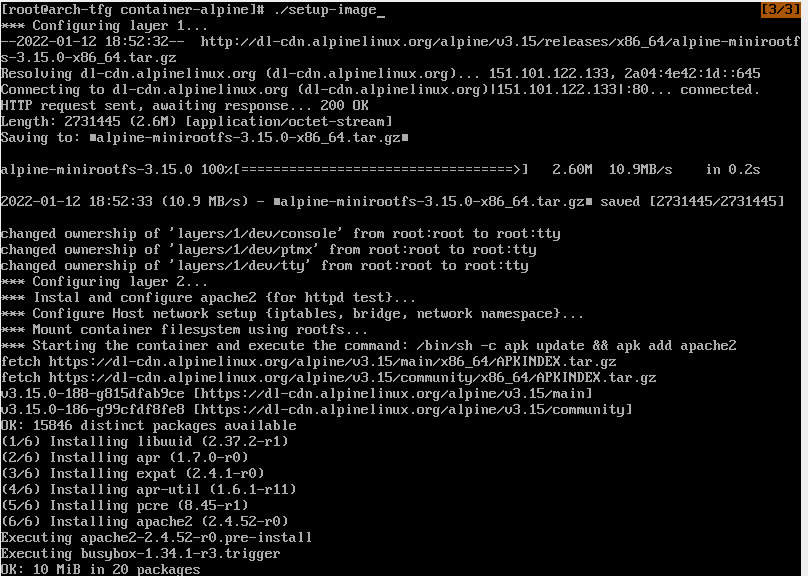
\includegraphics[width=0.9\textwidth]{img/container_setup1.png}
				\caption{Ejecución del script \texttt{setup-image} (1/2)}
			\end{center}
		\end{figure}
	
		\pagebreak
	
		\begin{figure}[h!]
			\begin{center}
				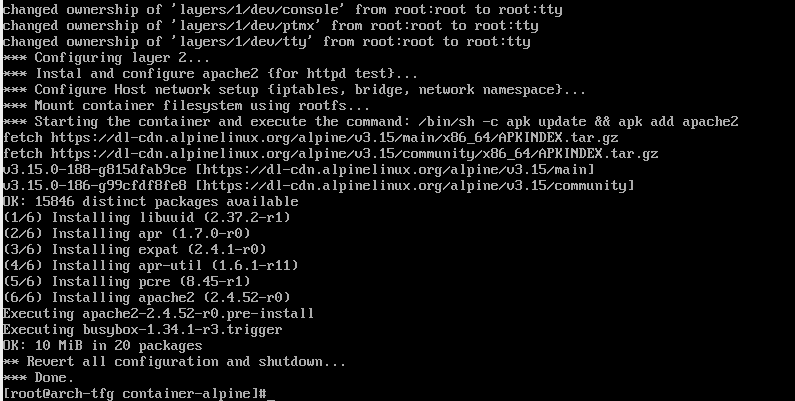
\includegraphics[width=0.9\textwidth]{img/container_setup2.png}
				\caption{Ejecución del script \texttt{setup-image} (2/2)}
			\end{center}
		\end{figure}
	
		%\pagebreak
		
		\item Una vez tenemos la imagen creada, ya podemos ejecutar el \texttt{runtime} con el comando que nosotros queramos. Para ello, tendremos que ejecutar el comando \texttt{./runtime-exec <commando>}
		
		\begin{figure}[h!]
			\begin{center}
				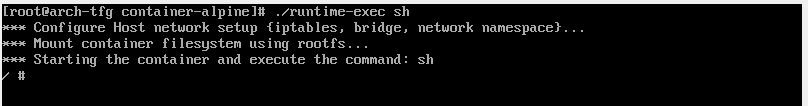
\includegraphics[width=1\textwidth]{img/container_runtime1.png}
				\caption{Ejecución del script \texttt{runtime-exec} (1/2)}
			\end{center}
		\end{figure}
	
		\noindent Dado que ya estamos dentro de una shell del contenedor, podemos comprobar como solo podemos ver los procesos del contenedor, y solo tenemos la interfaz de red asignada al contenedor.
		
		\begin{figure}[h!]
			\begin{center}
				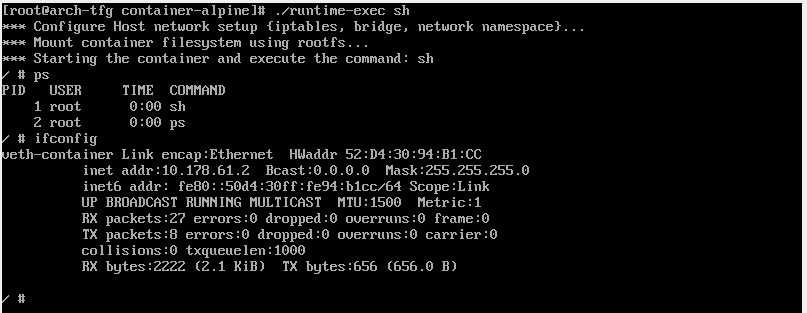
\includegraphics[width=0.85\textwidth]{img/container_runtime2.png}
				\caption{Ejecución del script \texttt{runtime-exec} (2/2)}
			\end{center}
		\end{figure}
	
		\item Ejecutamos el comando \texttt{httpd} y comprobamos que el host puede acceder al servicio. \\
		
		\noindent Como podemos comprobar en la siguiente imagen, el comando \texttt{httpd} se ejecuta correctamente en el contenedor. Por otro lado, utilizamos la herramienta \texttt{wget} para comprobar que tenemos acceso al servicio web que expone el comando \texttt{httpd}, el contenido del archivo \texttt{index.html} lo podemos ver también en las siguientes figuras.
		
		\pagebreak
		
		\begin{figure}[h!]
			\begin{center}
				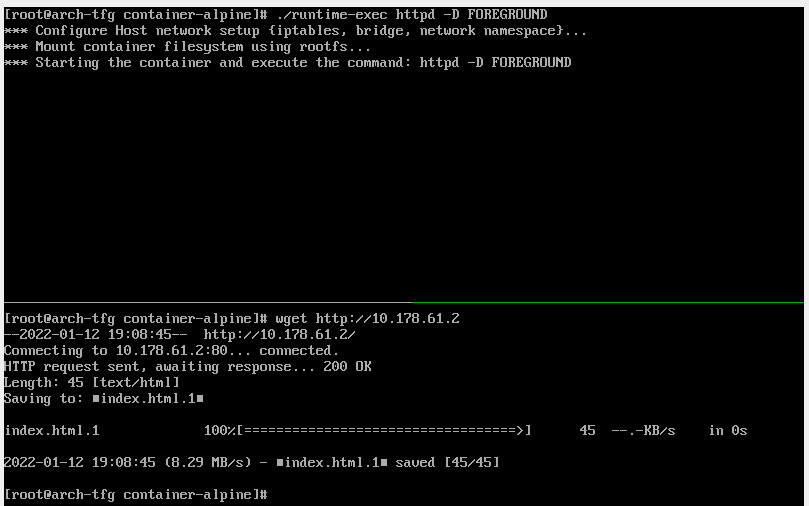
\includegraphics[width=0.8\textwidth]{img/container_runtime3.png}
				\caption{Ejecución del script \texttt{runtime-exec} con comando \texttt{httpd}}
			\end{center}
		\end{figure}
	
		\begin{figure}[h!]
			\begin{center}
				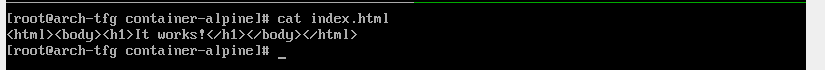
\includegraphics[width=0.75\textwidth]{img/container_runtime4.png}
				\caption{Ejecución del script \texttt{runtime-exec} con comando \texttt{httpd}}
			\end{center}
		\end{figure}
		
		\noindent Por lo tanto, podemos concluir que este ejemplo es válido para demostrar el funcionamiento de un contenedor, basado en namespaces y en sistemas de montaje de capas.
		
	\end{enumerate}
	
	\pagebreak
	
	\subsection{Contenedores \texttt{LXC}}
	\noindent En este apartado vamos a comentar la aplicación de contenedores LXC, LinuX Containers. Como bien hemos comentado en el apartado anterior, LXC consiste en una virtualización a nivel de sistema operativo (virtualización ligera), creada por el proyecto \url{linuxcontainers.org}, con el objetivo de poder ejecutar diferentes espacios aislados (contenedores) utilizando un único host, lo llamaremos LXC host. Aunque pueda parecer que estamos ante una técnica de virtualización basada en máquinas virtuales, se trata de espacios virtuales, en los que cada uno dispone de su propia CPU, memoria, redes, etc. Esto lo consigue gracias al uso de los \texttt{namespaces} y los \texttt{cgroups} en el host LXC. [\ref{bib: LXC arch}]. Algunas de las características más destacables son:
	\begin{itemize}
		\item Utiliza mount namespace para conseguir la estructura de directorios propia de una distribución de Linux.
		\item El proceso asignado a cada namespaces es el \texttt{init}, por lo tanto tendremos un proceso de arranque del sistema.
		\item Tiene sus propios usuarios, incluido un usuario root.
		\item Una vez dentro del contenedor, podemos instalar aplicaciones utilizando el gestor de paquetes de la distribución (\texttt{apt}, \texttt{zipper}, \texttt{pacman}, etc...)
	\end{itemize}

	\begin{figure}[h]
		\begin{center}
			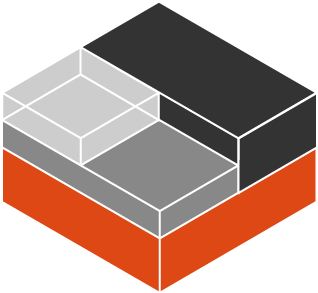
\includegraphics[width=0.2\textwidth]{img/lxc_logo.png}
			\caption{Logotipo del proyecto \url{linuxcontainers.org} [\ref{bib_img: lxc logo}]}
		\end{center}
	\end{figure}

	\noindent \textbf{\large Contenedores sin privilegios}\\

	\noindent Una característica muy importante de este tipo de contenedores es que permiten la posibilidad de configurar contenedores de dos tipos: contenedores con privilegios y contenedores sin privilegios. Esto es importante ya que si definimos un contenedor con privilegios, hay ciertas acciones que nos permitirían realizar comandos en el host. En el caso de que nuestro contenedor sea distribuido por terceros, puede suponer un problema grave de seguridad, ya que un atacante podría tomar el control de nuestro contenedor, y por consiguiente, también podría acceder a la información del host. Es por esto por lo que surge el concepto de contenedores sin privilegios (\textit{unprivileged containers}), considerados como una técnica mucho más segura ya que disponen de un nivel añadido de aislamiento respecto al host. La clave reside en ``mapear'' el UID del usuario \texttt{root} de nuestro contenedor a un UID del host que no tenga permisos de administrador. Por lo tanto, si un atacante consigue acceder a nuestro contenedor, y pudiera acceder al host, se vería con que no tiene permisos para realizar ninguna acción. [\ref{bib: LXC arch}]
	
	\pagebreak
	
	\noindent \textbf{\large Tipos de configuración de red en el host}\\
	
	\noindent LXC soporta dos tipos de conexiones virtuales de red. Estas son las siguientes: 
	\begin{itemize}
		\item NAT bridge. En este modo, LXC tiene su propio bridge (\texttt{lxcbr0}) que funciona en conjunto con las aplicaciones \texttt{dnsmasq} e \texttt{iptables} del host, dando lugar a que se puedan utilizar servicios red como DNS, DHCP y NAT dentro del propio contenedor.
		\item Host bridge. En este modo, ese necesario que el host configure su propio bridge para dar servicio a las aplicaciones que creamos pertinentes. Esta opción nos permite mucha flexibilidad a la hora de interconectar nuestros contenedores para una funcionalidad específica.
	\end{itemize}


	\vspace{20px}

	\noindent \textbf{\large Utilizar NAT bridge en un contenedor}\\

	\noindent A modo de ejemplo, si quisiéramos utilizar redes tipo NAT bridge en un contenedor [\ref{bib: LXC arch}], primero tendríamos que crear el archivo \texttt{/etc/default/lxc-net} con el siguiente contenido:
	\begin{lstlisting}[language=Bash, caption={Configuración interfaz NAT bridge en LXC}]
# Leave USE_LXC_BRIDGE as "true" if you want to use lxcbr0 for your
# containers.  Set to "false" if you'll use virbr0 or another existing
# bridge, or mavlan to your host's NIC.
USE_LXC_BRIDGE="true"

# If you change the LXC_BRIDGE to something other than lxcbr0, then
# you will also need to update your /etc/lxc/default.conf as well as the
# configuration (/var/lib/lxc/<container>/config) for any containers
# already created using the default config to reflect the new bridge
# name.
# If you have the dnsmasq daemon installed, you'll also have to update
# /etc/dnsmasq.d/lxc and restart the system wide dnsmasq daemon.
LXC_BRIDGE="lxcbr0"
LXC_ADDR="10.0.3.1"
LXC_NETMASK="255.255.255.0"
LXC_NETWORK="10.0.3.0/24"
LXC_DHCP_RANGE="10.0.3.2,10.0.3.254"
LXC_DHCP_MAX="253"
# Uncomment the next line if you'd like to use a conf-file for the lxcbr0
# dnsmasq.  For instance, you can use 'dhcp-host=mail1,10.0.3.100' to have
# container 'mail1' always get ip address 10.0.3.100.
#LXC_DHCP_CONFILE=/etc/lxc/dnsmasq.conf

# Uncomment the next line if you want lxcbr0's dnsmasq to resolve the .lxc
# domain.  You can then add "server=/lxc/10.0.3.1' (or your actual $LXC_ADDR)
# to your system dnsmasq configuration file (normally /etc/dnsmasq.conf,
# or /etc/NetworkManager/dnsmasq.d/lxc.conf on systems that use NetworkManager).
# Once these changes are made, restart the lxc-net and network-manager services.
# 'container1.lxc' will then resolve on your host.
#LXC_DOMAIN="lxc"
	\end{lstlisting}

	\pagebreak

	\noindent Ahora, necesitamos modificar la \textit{template} del contenedor LXC para que utilice la interfaz que hemos configurado. Modificamos la plantilla con ruta \texttt{/etc/lxc/default.conf} tal que:
	\begin{lstlisting}[language=Bash, caption={Configuración contenedor LXC para usar NAT bridge}]
lxc.net.0.type = veth
lxc.net.0.link = lxcbr0
lxc.net.0.flags = up
lxc.net.0.hwaddr = 00:16:3e:xx:xx:xx
	\end{lstlisting}

	\noindent Para que todos estos cambios se realicen, es necesario que tengamos activado el servicio \texttt{lxc-net.service}.
	\begin{verbatim}
> sudo systemctl enable lxc-net.service
> sudo systemctl start lxc-net.service
	\end{verbatim}

	\vspace{20px}

	\noindent \textbf{\large Crear un contenedor con privilegios utilizando LXC}\\
	
	\noindent Si decidimos crear un contenedor con privilegios, tendríamos que seguir los siguientes pasos [\ref{bib: crear LXC}]:
	\begin{lstlisting}[language=Bash, caption={Crear un contenedor con privilegios en LXC}]
sudo lxc-create --template download --name <NombreContenedor>
	\end{lstlisting}

	\noindent Con este comando, LXC nos preguntará de manera interactiva por un \texttt{root filesystem} para el contenedor a descargar, además de la distribución elegida, la versión o la arquitectura. Si queremos hacerlo de manera que no sea interactivo, podemos crear el contenedor tal que:
	\begin{lstlisting}[language=Bash, caption={Crear un contendor con privilegios en LXC, modo no interactivo}]
sudo lxc-create --template download --name <NombreContenedor> -- --dist debian --release stretch --arch amd64
	\end{lstlisting}

	\noindent De esta manera, ya tendríamos creado nuestro contenedor. Para poder manejar dichos contenedores, es conveniente conocer los comandos disponibles por LXC. Algunos de los más importantes son los siguientes [\ref{bib: crear LXC}]:
	\begin{itemize}
		\item \texttt{sudo lxc-ls --fancy}. Lista los contenedores disponibles por el host.
		\item \texttt{sudo lxc-info --name <NombreContenedor>}. Permite conocer la información de un contenedor específico.
		\item \texttt{sudo lxc-attach --name <NombreContenedor>}. Nos conecta directamente con la shell de nuestro contenedor.
		\item \texttt{sudo lxc-start --name <NombreContenedor> --daemon}. Permite arrancar el contenedor.
		\item \texttt{sudo lxc-stop --name <NombreContendor>}. Permite parar un contenedor que esté en ejecución.
		\item \texttt{sudo lxc-destroy --name <NombreContenedor>}. Elimina un contenedor, incluido su directorio \texttt{root}.
	\end{itemize}
	
	\pagebreak
	
	\noindent Una vez creamos el contenedor, es interesante modificar su configuración para asignarle una interfaz de red. Esto lo haremos modificando el archivo config con ruta: 
	\begin{verbatim}
/var/lib/lxc/<NombreContenedor>/config
	\end{verbatim}
	\noindent Añadiremos la siguiente configuración para que utilice el \texttt{NAT bridge} que definimos con anterioridad, además de permitir la ejecución de aplicaciones tipo X11, utilizando xorg (aplicaciones con interfaz gráfica) [\ref{bib: xorg arch wiki}].
	\begin{lstlisting}[language=Bash, caption={Configuración interfaz NAT bridge y aplicaciones X a un contenedor LXC}]
# Network configuration (bridge)
lxc.net.0.type = veth
lxc.net.0.veth.pair = veth_containerLXC
lxc.net.0.flags = up
lxc.net.0.ipv4.address = 172.16.27.2/24

## for xorg
lxc.mount.entry = /dev/dri dev/dri none bind,optional,create=dir
lxc.mount.entry = /dev/snd dev/snd none bind,optional,create=dir
lxc.mount.entry = /tmp/.X11-unix tmp/.X11-unix none bind,optional,create=dir,ro
lxc.mount.entry = /dev/video0 dev/video0 none bind,optional,create=file
	\end{lstlisting}
	
	\noindent Ahora ya tenemos listo el contenedor para arrancarlo, solo nos quedaría asignar una IP válida al host, que también está dentro del \texttt{bridge} de LXC. Para ello, ejecutaremos:
	\begin{lstlisting}[language=Bash, caption={Asignar IP al host LXC y arrancar un contenedor}]
ip link add 172.16.27.1/24 dev veth_containerLXC
sudo lxc-start --name <NombreContenedor>
sudo lxc-attach --name <NombreContenedor>

# Para ejecutar interfaz grafica
startx
	\end{lstlisting}

	\vspace{20px}

	\noindent \textbf{\large Crear un contenedor sin privilegios utilizando LXC}\\
	
	\noindent En el caso de optar por la opción más segura, que es la de crear un contenedor sin privilegios en el host. Tendremos que realizar una serie de configuraciones previas [\ref{bib: unprivileged LXC}]. La primera consistirá en crear un usuario sin privilegios para LXC:
	\begin{verbatim}
$ sudo useradd -s /bin/bash -c 'unprivileged lxc user' -m lxc_user
$ sudo passwd lxc_user
	\end{verbatim}

	\noindent Ahora, necesitamos buscar los valores de grupo (subgid) e identificación (subuid) del usuario creado, para ello ejecutamos lo siguiente:
	\begin{verbatim}
$ sudo grep lxc_user /etc/sub{gid,uid}
	\end{verbatim}

	\noindent Obteniendo por consola una salida similar a la siguiente:
	\begin{verbatim}
/etc/subgid:lxc_user:100000:65536
/etc/subuid:lxc_user:100000:65536
	\end{verbatim}

	\pagebreak
	
	\noindent Utilizando las mismas configuraciones de red que en el aparatado de contenedor con privilegios, procedemos a acceder al usuario asignado a LXC. Ejecutaremos el comando \texttt{id} para conocer los diferentes \texttt{uid} y \texttt{gid} asignados.
	\begin{verbatim}
$ su lxc_user
$ id
	\end{verbatim}

	\noindent Tendremos una salida similar a:
	\begin{verbatim}
uid=1002(lxc_user) gid=1002(lxc_user) groups=1002(lxc_user)
	\end{verbatim}

	\noindent El siguiente paso sería crear los directorios de configuración de LXC, y copiar la configuración \textit{default} a dichos directorios.
	\begin{verbatim}
$ mkdir -p /home/lxc_user/.config/lxc
$ cp /etc/lxc/default.conf /home/lxc_user/.config/lxc/default.conf
	\end{verbatim}

	\noindent Por último, tendríamos que modificar dicho archivo para realizar un ``mapeo de permisos''. Con el fin de asignar la ejecución del contenedor al usuario LXC que acabamos de crear. Al final del archivo \texttt{default.conf} que acabamos de copiar, añadimos lo siguiente:
	\begin{lstlisting}[language=Bash, caption={Configuración para mapear UID y GID para un contenedor sin privilegios en LXC}]
lxc.id_map = u 0 100000 65536
lxc.id_map = g 0 100000 65536
	\end{lstlisting}

	\noindent Una vez realizados todos estos pasos, ya podríamos crear nuestro contenedor sin privilegios. Lo haríamos de manera similar que en el apartado anterior, es decir utilizando el comando \texttt{lxc-create}. Además, también será importante modificar el archivo \texttt{config} de nuestro contenedor para asignar la interfaz de red y permitir la ejecución de aplicaciones con interfaz gráfica. \\
	
	%\vspace{10px}
	\pagebreak
	
	\noindent \textbf{\large Ejemplo: \texttt{namespaces} en un contenedor LXC de Ubuntu}\\
	
	\noindent A modo de ejemplo, vamos a crear un contenedor (con privilegios) paso a paso, y por último, vamos a verificar que namespaces está utilizando dicho contenedor. Para esto, vamos a crear un contenedor de Ubuntu 20.04.03 (Focal) utilizando el catálogo de imágenes de LXC.
	
	%https://www.alibabacloud.com/blog/how-to-install-and-configure-lxc-container-on-ubuntu-16-04_594090
	\begin{enumerate}
		\item Lo primero que tenemos que hacer es verificar que LXC está instalado correctamente en nuestro sistema, una manera fácil de comprobarlo es con el siguiente comando:
		\begin{verbatim}
			$ sudo lxc-checkconfig
		\end{verbatim}
	
		\begin{figure}[h!]
			\begin{center}
				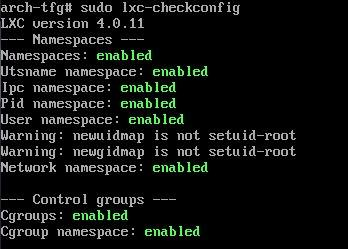
\includegraphics[width=0.36\textwidth]{img/lxc_ns1.jpg}
				\caption{Comprobación instalación de LXC usando \texttt{lxc-checkconfig}}
			\end{center}
		\end{figure}
	
		\item Creamos el contenedor de Ubuntu siguiendo los pasos de la creación guiada de contenedores que hemos comentado en apartados anteriores.
		\begin{verbatim}
			$ sudo lxc-create --template download --name <NombreContenedor>
		\end{verbatim}
		
		\begin{figure}[h!]
			\begin{center}
				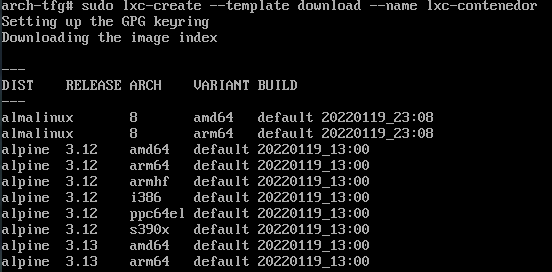
\includegraphics[width=0.7\textwidth]{img/lxc_ns2.png}
				\caption{Instalación de contenedor LXC (1)}
			\end{center}
		\end{figure}
		
		\pagebreak
		
		\noindent De manera interactiva, el programa nos preguntará por diferentes opciones para nuestro contenedor. Para elegir una distribución, podemos acceder a la siguiente web: \href{https://uk.lxd.images.canonical.com/}{imagenes LXC}, en las que aparecen todas las imagenes disponibles. En este caso, escribimos lo siguiente para cada una de ellas:
		\begin{itemize}
			\item \textit{Distribution}: \texttt{ubuntu}
			\item \textit{Release}: \texttt{focal}
			\item \textit{Architecture}: \texttt{amd64}
		\end{itemize}
	
		\begin{figure}[h!]
			\begin{center}
				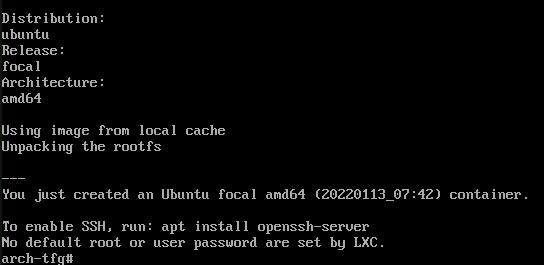
\includegraphics[width=0.7\textwidth]{img/lxc_ns3.png}
				\caption{Instalación de contenedor LXC (2)}
			\end{center}
		\end{figure}
	
		\item Iniciamos el contenedor que acabamos de crear.
		\begin{verbatim}
			$ sudo lxc-start -n <NombreContenedor> -d
		\end{verbatim}
	
		\item Accedemos a la terminal del contenedor que acabamos de iniciar.
		\begin{verbatim}
			$ sudo lxc-attach -n <NombreContenedor>
		\end{verbatim}
	
		\item Una vez dentro del contenedor de Ubuntu, podemos comprobar con el siguiente comando que efectivamente se ha instalado la distribución que hemos elegido.
		\begin{verbatim}
			$ cat /etc/os-release
		\end{verbatim}
	
		\begin{figure}[h!]
			\begin{center}
				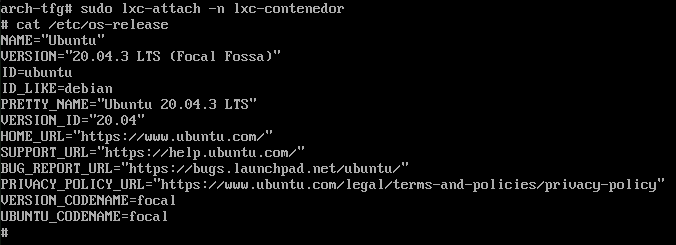
\includegraphics[width=0.85\textwidth]{img/lxc_ns4.png}
				\caption{Comprobación de la versión de Ubuntu instalada en el contenedor LXC}
			\end{center}
		\end{figure}
	
		\pagebreak
	
		\item Por último, en otra terminal, procedemos a obtener el \texttt{PID} asociado a dicho contenedor. Para ello, podemos hacer uso del siguiente comando:
		\begin{verbatim}
			$ sudo lxc-info -p -n <NombreContenedor>
		\end{verbatim}
	
		\noindent Una vez tenemos el PID, podemos utilizar el comando \texttt{lsns} los namespaces que están asociados a dicho PID. Para ello, ejecutamos lo siguiente:
		\begin{verbatim}
			$ sudo lsns | grep <PID_contenedor>
		\end{verbatim}
	
		\begin{figure}[h!]
			\begin{center}
				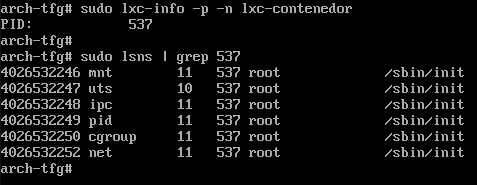
\includegraphics[width=0.7\textwidth]{img/lxc_ns5.png}
				\caption{Namespaces asociados a un contenedor LXC ejecutado en el host}
			\end{center}
		\end{figure}
	\end{enumerate}
	
	\pagebreak
	
	\subsection{Contenedores \texttt{Docker}}
	\label{sec: docker}
	\noindent En este apartado vamos a profundizar en la herramienta \texttt{Docker}. Al igual que en el caso de \texttt{LXC}, \texttt{Docker} permite la creación y la gestiones de aplicaciones aisladas entre sí, utilizando virtualización ligera; es decir, nos permite gestionar facilmente un entorno de contenedores. \\
	
	\noindent Tal y como lo definen sus creadores [\ref{bib: docker info}], \texttt{Docker} es una plataforma de desarrollo, despliegue y ejecución de aplicaciones. \texttt{Docker} permite separar entre aplicaciones de tu infraestructura, permitiendo desplegar el software mucho más rápido. Uno de los objetivos que persigue esta plataforma es el de minimizar el tiempo entre programar y tener ejecutando la aplicación en producción. Algunas de las ventajas que nos aporta esta plataforma son:
	\begin{itemize}
		\item Ejecutar aplicaciones de manera aislada, uso de contenedores.
		\item Desplegar un número elevado de contenedores en un mismo host.
		\item Contenedores ligeros y que además, contienen todo lo necesario para ejecutar la aplicación. Independientemente del host.
		\item Facilidad a la hora de compartir contenedores con otros compañeros.
		\item Equivalencia entre despliegue local y despliegue en producción.
	\end{itemize}

	\vspace{5px}
	\noindent \textbf{\large Arquitectura de \texttt{Docker}}\\
	
	\noindent \texttt{Docker} utiliza una arquitectura de cliente-servidor. El cliente de \texttt{Docker} se comunica con un ``demonio'' de la máquina host (servicio en ejecución en segundo plano), que tiene como funciones: crear, ejecutar y distribuir los contenedores \texttt{Docker}. Gracias a esta arquitectura, el cliente \texttt{Docker} puede estar en la misma máquina, o bien se puede conectar a un ``demonio'' remoto, esto se puede realizar utilizando una REST API (conectar a máquina remota) o bien UNIX sockets (conectar a máquina local)[\ref{bib: docker info}]. 
	
	\begin{figure}[h]
		\begin{center}
			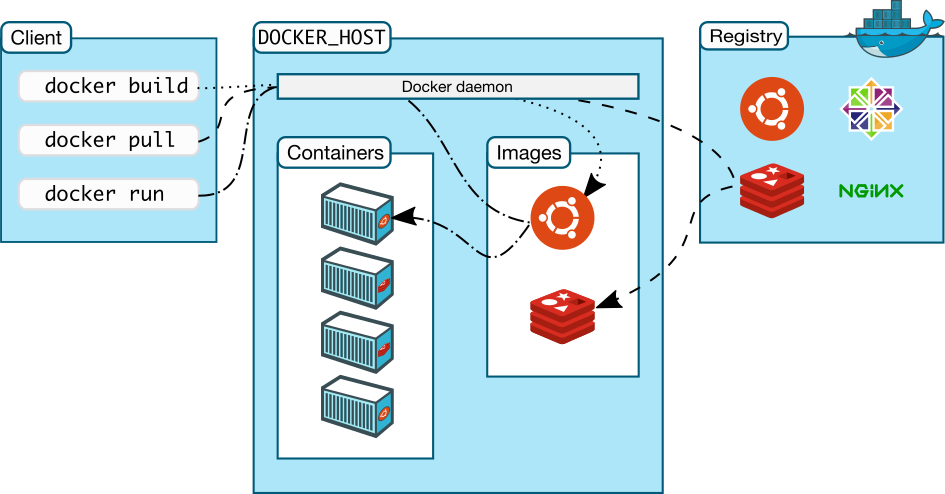
\includegraphics[width=0.675\textwidth]{img/architecture-docker.png}
			\caption{Arquitectura Docker [\ref{bib_img: docker arch}]}
		\end{center}
	\end{figure}
	
	\pagebreak
	
	\noindent \textbf{\large Tecnologías utilizadas por \texttt{Docker}}\\
	
	\noindent \texttt{Docker} está desarrollado en el lenguaje de programación Go (\url{https://golang.org/}), y utiliza las ventajas aportadas por el kernel de Linux para desarrollar su funcionalidad. Estas tecnologías son, los \texttt{namespaces}, explicados en el apartado \ref{sect: espacio nombres}, que nos permiten aislar los diferentes espacios de trabajo de nuestras aplicaciones; especialmente utilizarán \texttt{cgroups} para aplicar reglas a la hora de ejecutar cada contenedor. [\ref{bib: docker info}]
	
	\vspace{10px}
	
	\begin{figure}[h]
		\begin{center}
			
\includegraphics[width=0.6\textwidth]{img/docker_logo.png}
			\caption{Logotipo de Docker [\ref{bib_img: docker logo}]}
		\end{center}
	\end{figure}
	
	\vspace{10px}
	\noindent \textbf{\large Primeros pasos en \texttt{Docker}}\\
	
	\noindent Lo primero que tendremos que hacer para utilizar \texttt{Docker}, es proceder a instalar dicha herramienta. Para ello, tendríamos que seguir los pasos que se nos especifican en \url{https://docs.docker.com/get-docker/}. \\
	
	\noindent Una vez instalado, podemos comprobar que el ``demonio'' está funcionando si ejecutamos los siguientes comandos desde el cliente de docker.
	\begin{verbatim}
$ sudo docker version
	\end{verbatim}

	\noindent El comando nos devolverá información sobre el cliente de docker e intentará conectar con el ``demonio''. En el caso de que nos responda como en la imagen (\ref{img: docker version}), tendremos que ejecutar el comando:
	\begin{verbatim}
$ sudo systemctl start docker.service
	\end{verbatim}
	
	\begin{figure}[h]
		\begin{center}
			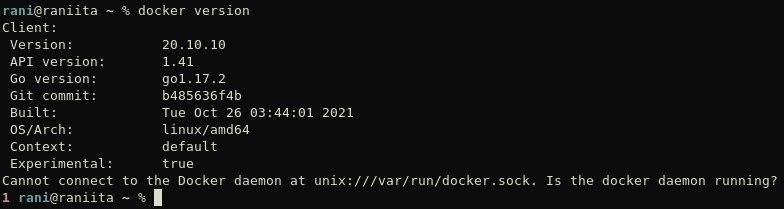
\includegraphics[width=0.9\textwidth]{img/docker_version.jpg}
			\caption{Ejecución comando \texttt{docker version} sin ``demonio'' en funcionamiento}
			\label{img: docker version}
		\end{center}
	\end{figure}

	\pagebreak
	
	\noindent Una vez comprobado que tenemos conexión con el ``daemon''. Lo siguiente, será ejecutar nuestro primer contenedor. En este caso, haremos uso de un contenedor ``especial" que nos verifica la instalación de docker en nuestros host. Para ello, ejecutamos el siguiente comando:
	\begin{verbatim}
$ docker run hello-world
	\end{verbatim}

	\noindent Una vez termina de ejecutarse el comando, la salida por consola que obtendremos sería equivalente a la siguiente figura:
	
	\begin{figure}[h]
		\begin{center}
			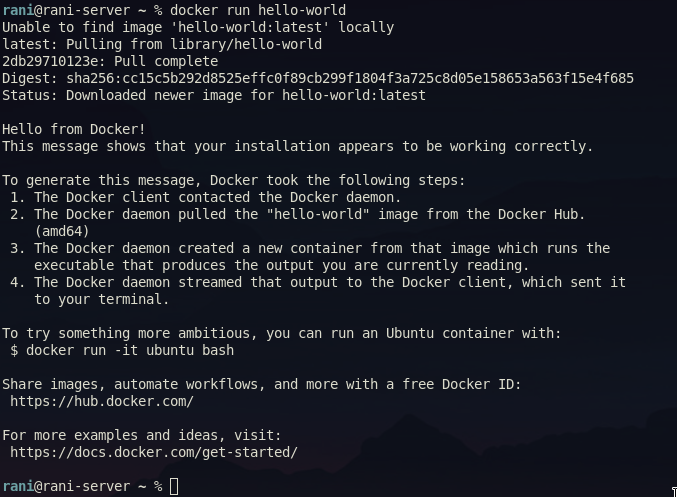
\includegraphics[width=0.8\textwidth]{img/docker_hello-world.png}
			\caption{Ejecución comando \texttt{docker run hello-world} para comprobar instalación}
			\label{img: docker hello world}
		\end{center}
	\end{figure}

	\noindent Como podemos ver en la figura \ref{img: docker hello world}, el contenedor nos muestra por consola los pasos que ha seguido para completar su ejecución. Antes de comentar los pasos seguidos, es importante aclarar el concepto de ``imagen''. \\
	
	\noindent Llamamos imagen de Docker a un archivo de sistema, compuesto por diferentes capas de información, que es utilizado para desplegar un contenedor de Docker. Entendemos estas imágenes como la plantilla base desde la que partimos para crear nuevos contenedores para ejecutar aplicaciones, o bien para crear una nueva imagen.\\
	
	\pagebreak
	
	\noindent Una vez estamos familiarizados con el concepto de imagen, podemos proceder a comentar los pasos realizados por Docker para mostrarnos el mensaje de la figura \ref{img: docker hello world}. Dichos pasos serían los siguientes:
	\begin{enumerate}
		\item El cliente de docker contacta con el ``daemon'' de docker.
		\item El ``daemon'' descarga la imagen  ``hello-world'' del respositorio público de imagenes de docker (Docker Hub).
		\item El ``daemon'' crea un nuevo contenedor a partir de esa imagen, que correrá un ejecutable que producen la salida que hemos obtenido.
		\item El ``daemon'' envia la información de salida del contendor al cliente de docker, permitiendo al usuario ver la salida en su terminal.
	\end{enumerate}

	\noindent Por otro lado, en esa misma ejecutión del contendor ``hello-world'', se nos invita a ejecutar lo siguiente:
	\begin{verbatim}
$ docker run -it ubuntu bash
	\end{verbatim}

	\noindent Si analizamos la sintaxis del comando anterior, podemos diferenciar entre cinco elementos diferentes:
	\begin{itemize}
		\item \texttt{docker}. Binario de la máquina linux, corresponde con el cliente de docker.
		\item \texttt{run}. Argumento del cliente de docker, permite crear y ejecutar un contenedor.
		\item \texttt{-it}. Opciones del argumento \texttt{run}. En este caso, tenemos configurado que sea de tipo interactivo (\texttt{-i}), es decir que nos muestre por consola la salida del comando; y además, hemos seleccionado que configure el terminal como un terminal dentro del contenedor que vamos a crear (\texttt{-t}).
		\item \texttt{ubuntu}. Imagen que hemos elegido para nuestro contenedor. Primero la buscará localmente, y si no la encuentra, comprobará en el repositorio público de imágenes (Docker Hub).
		\item \texttt{bash}. Binario a ejecutar dentro del contenedor, en este caso corresponde con una consola shell.
	\end{itemize}

	\noindent Una vez ejecutamos dicho comando, automáticamente se crea un contendor con una imagen de \texttt{ubuntu} y se nos ejecuta una consola, en la que podemos navegar y trabajar de manera aislada a nuestra máquina host. (ver Figuras \ref{img: docker ubuntu} y \ref{img: docker ubuntu ver}).
	
	\pagebreak
	
	\begin{figure}[h]
		\begin{center}
			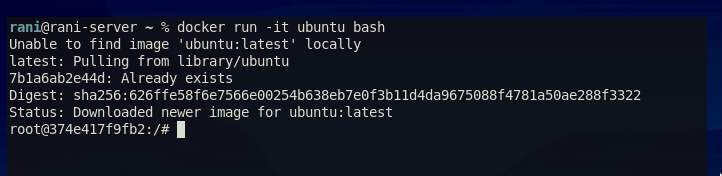
\includegraphics[width=0.9\textwidth]{img/docker_ubuntu.png}
			\caption{Ejecución comando \texttt{docker run -it ubuntu bash} para levantar un contenedor ubuntu}
			\label{img: docker ubuntu}
		\end{center}
	\end{figure}


	\noindent Para comprobar que estamos en una distribución ubuntu, y además ver la versión que el docker ``daemon'' ha descargado, ejecutamos el comando siguiente. Como podemos comprobar, el contenedor está utilizando la última versión LTS (Long Term Support, versiones más estables y probadas que tendrán soporte durante un largo periodo de tiempo) disponible hasta la fecha.
	
	\begin{figure}[h]
		\begin{center}
			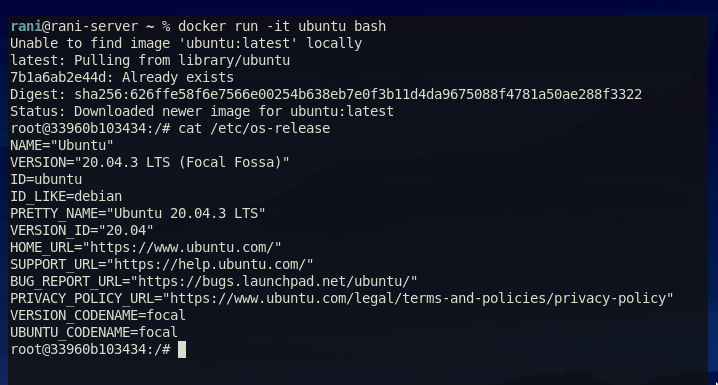
\includegraphics[width=0.9\textwidth]{img/docker_ubuntu_ver.png}
			\caption{Comprobación de la versión de ubuntu del contenedor desplegado}
			\label{img: docker ubuntu ver}
		\end{center}
	\end{figure}

	\pagebreak

	%\vspace{10px}
	\noindent \textbf{\large Concepto de \texttt{Dockerfile}. Primer contenedor}\\
	
	\noindent En este apartado, a modo de ejemplo, vamos a crear nuestro propio contenedor en el que correremos una aplicación de Python muy sencilla [\ref{bib: docker dockerfile}]. Para ello, primero vamos a crear una carpeta en nuestro ordenador, en ella crearemos dos archivos:
	\begin{itemize}
		\item Uno se llamará \texttt{main.py} y contendrá el código que será ejecutado en el contenedor.
		\item Otro llamado \texttt{Dockerfile}, en el que detallaremos las instrucciones que tiene que seguir docker para crear nuestro contenedor.
	\end{itemize}

	\noindent Por lo tanto, la carpeta nos quedaría tal que así (ver Figura [\ref{img: docker file folder}]):
	
	\begin{figure}[h]
		\begin{center}
			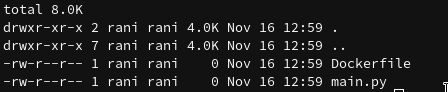
\includegraphics[width=0.7\textwidth]{img/dockerfile_folder.png}
			\caption{Comprobación de la versión de ubuntu del contenedor desplegado}
			\label{img: docker file folder}
		\end{center}
	\end{figure}
	
	\begin{enumerate}
		\item Primero procedemos a editar el archivo Python \texttt{main.py}, para ello utilizamos el siguiente código:
		\begin{lstlisting}[language=Python, caption=Codigo Python de ejemplo para crear un Dockerfile]
#!/usr/bin/env python3

print("Saludos desde tu contendor!!")
		\end{lstlisting}
	
		\item Ahora procederemos a la parte de modificar el \texttt{Dockerfile}. \\
		
		\noindent Lo primero que tenemos que tener claro es lo que queremos que haga nuestro contenedor. En este caso sería que ejecutase el código Python de \texttt{main.py}, en otro caso podría ser que quisiéramos desplegar otro tipo de aplicación. Para hacer esto, primero tenemos que buscar una imagen que nos sirva de base para construir nuestro contenedor. En el caso de Python, nos podría servir un \texttt{ubuntu}, ya que viene con Python preinstalado, sin embargo, vamos a buscar una imagen mucho más especifica. Para ello, nos dirigimos a la página de \texttt{DockerHub} \url{https://hub.docker.com/} y buscamos Python en el buscador (ver Figura \ref{img: dockerhub python}).
	
	\pagebreak
	
	\begin{figure}[h]
		\begin{center}
			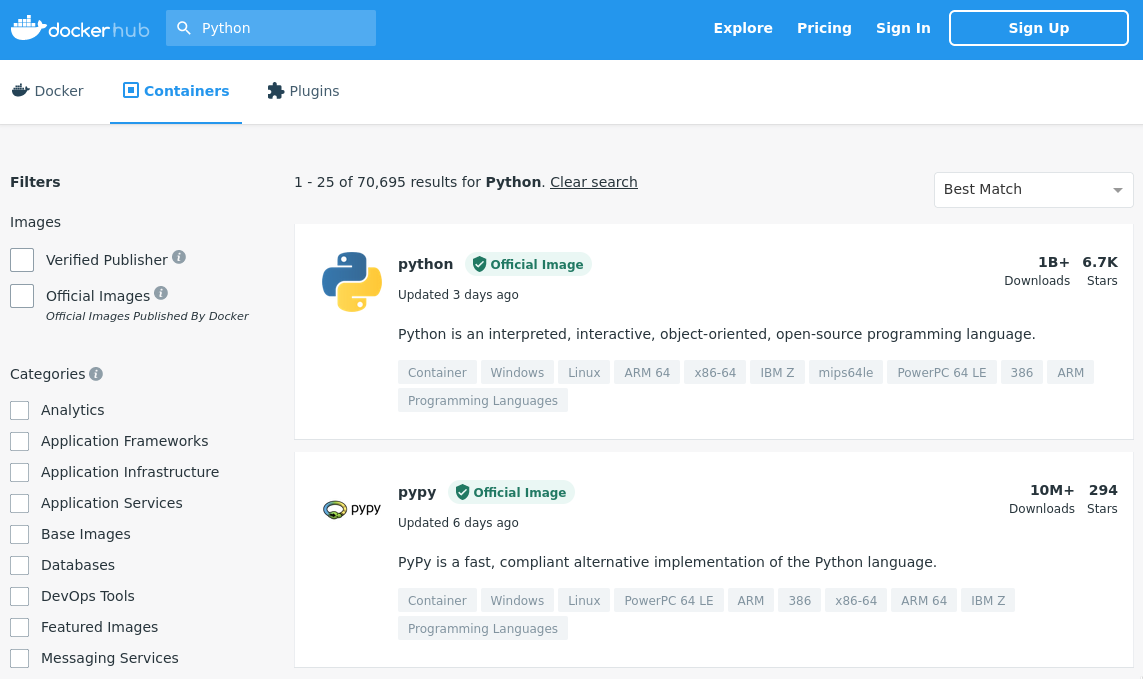
\includegraphics[width=0.9\textwidth]{img/dockerhub_python.png}
			\caption{Búsqueda en \texttt{DockerHub} de una imagen base para nuestro contenedor.}
			\label{img: dockerhub python}
		\end{center}
	\end{figure}
	
	\noindent El primer resultado que obtenemos es el de una imagen de contenedor que nos permite ejecutar código Python. Además, podemos ver como es muy apoyada por la comunidad (dato importante de cara a al estabilidad y seguridad de nuestro contenedor). Por lo tanto, usaremos la imagen \texttt{python} para utilizarla como base de nuestro contenedor. Ahora, procedemos a editar el archivo \texttt{Dockerfile} tal que así:
	\begin{lstlisting}[language=bash, caption={Contenido del archivo Dockerfile para crear contenedor con código Python}]
		# Un Dockerfile siempre necesita importar una imagen como base
		# Para ello utilizamos 'FROM'
		# Elegimos 'python' para la imagen y 'latest' como version de esa imagen
		FROM python:latest
		
		# Para ejecutar nuestro codigo Python, lo copiamos dentro del contenedor
		# Para ello utilizamos 'COPY'
		# El primer parametro 'main.py' es la ruta origen del archivo en el host
		# El segundo parametro '/' es la ruta destino del archivo dentro del contenedor
		# En este caso, ponemos el archivo en el root del sistema
		COPY main.py /
		
		# Definimos el comando a ejecutar cuando iniciemos el contenedor
		# Para ello utilizamos 'CMD'
		# Para ejecutar la aplicacion utilizariamos "python ./main.py".
		CMD [ "python", "./main.py" ]
	\end{lstlisting}
	
	\pagebreak
	
	\item Una vez tenemos los dos archivos, ya podemos crear la imagen de nuestro contenedor (ver Figura \ref{img: dockerfile python build}). Para ello, tenemos que ejecutar el siguiente comando:
	\begin{verbatim}
$ docker build -t python-hello_world .
	\end{verbatim}

	\noindent La opción \texttt{-t} nos permite asignar un nombre a nuestra imagen, en nuestro caso hemos elegido \texttt{python-hello\_world}.
	
	\item Ya tenemos nuestra imagen creada, por lo que podemos ejecutar nuestro contenedor y comprobar que nuestro código Python se ejecuta correctamente. Para lanzar el contenedor ejecutamos el siguiente comando:
	\begin{verbatim}
$ docker run python-hello_world
	\end{verbatim}

	\noindent En la terminal deberíamos comprobar el código se ha ejecutado correctamente (ver Figura \ref{img: dockerfile python run}).
	
	\begin{figure}[h]
		\begin{center}
			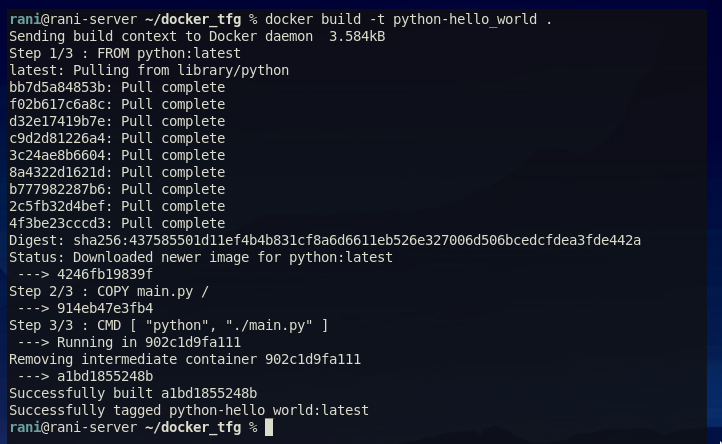
\includegraphics[width=0.82\textwidth]{img/dockerfile_build.png}
			\caption{Creación de imagen Docker para aplicación Python de pruebas}
			\label{img: dockerfile python build}
		\end{center}
	\end{figure}

	\begin{figure}[h]
		\begin{center}
			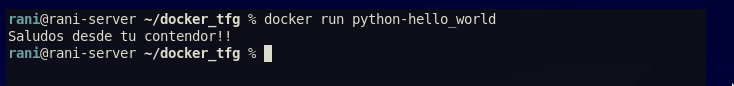
\includegraphics[width=0.85\textwidth]{img/dockerfile_run.png}
			\caption{Ejecución de la imagen Docker creada, utilizando \texttt{Dockerfile}}
			\label{img: dockerfile python run}
		\end{center}
	\end{figure}
	
	\end{enumerate}
	
	\pagebreak
	
	\noindent \textbf{\large Ejemplo: \texttt{network namespace} asociado a un contenedor Docker}\\
	
	\noindent A modo de comprobación de que en efecto Docker utiliza namespaces para la creación de sus contenedores, vamos a profundizar en como obtener los namespaces asociados a un contenedor en específico. [\ref{bib: docker y namespaces}] \\
	
	\noindent Primero, vamos a iniciar un contenedor con la imagen de Docker Alpine:
	
	\begin{verbatim}
$ docker pull alpine
$ docker run -d --name docker-ns alpine sleep 3600d
$ docker ps | grep alpine
	\end{verbatim}

	\begin{figure}[h!]
		\begin{center}
			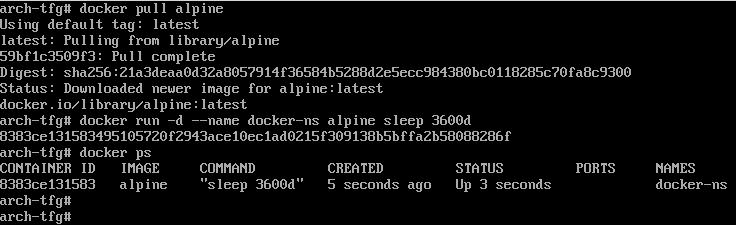
\includegraphics[width=0.9\textwidth]{img/docker_ns1.png}
			\caption{Ejecución contenedor Docker para ver sus namespaces asociados.}
		\end{center}
	\end{figure}

	\noindent Si ejecutamos el comando \texttt{ip netns list}, podemos comprobar como nos devuelve una lista vacía. De primeras, podríamos entender esto como que Docker no utiliza network namespaces, sin embargo, esto pasa porque Docker ``esconde'' estos namespaces por defecto.
	
	\begin{figure}[h!]
		\begin{center}
			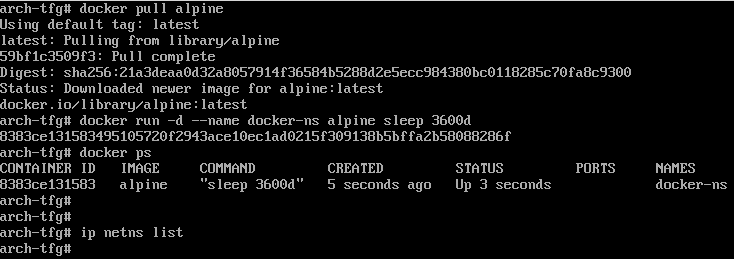
\includegraphics[width=0.9\textwidth]{img/docker_ns2.png}
			\caption{Resultado de comando \texttt{ip netns list} con contenedores Docker.}
			\end{center}
	\end{figure}

	\pagebreak
	
	\noindent Si queremos exponer los namespaces de un contenedor, tenemos que hacerlo manualmente. Para ello, utilizamos los siguientes comandos:
	
	\begin{verbatim}
$ sudo docker inspect -f '{{.State.Pid}}' docker-ns

$ ln -s /proc/<Pid>/ns/net /var/run/netns/<Pid>
	\end{verbatim}

	\begin{figure}[h!]
		\begin{center}
			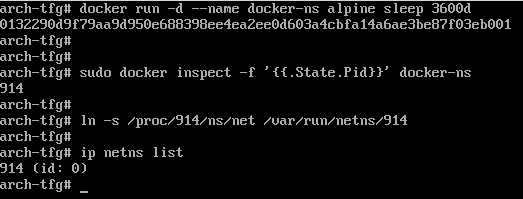
\includegraphics[width=0.8\textwidth]{img/docker_ns3.png}
			\caption{Network namespaces de un Docker container}
		\end{center}
	\end{figure}

	\noindent Una vez ya nos aparece el network namespace dentro del comando \texttt{ip netns list}, podemos comprobar que en efecto es el namespace asociado a nuestro contenedor, para ello podemos ejecutar los siguientes comandos:
	
	\begin{verbatim}
$ ip netns exec <ip netns output> ip address
	\end{verbatim}

	\noindent Que tiene que dar una salida equivalente a los siguientes comandos:
	
	\begin{verbatim}
$ docker exec -it docker-ns sh
/ ip address
	\end{verbatim}

	\noindent Tal y como podemos ver en la figura \ref{img: comprobacion ns docker}, ambos comandos dan el mismo resultado, por lo que quedaría comprobado que Docker utiliza network namespaces para dar conectividad a sus contenedores. Además, es interesante como ``esconde'' los identificadores de los namespaces que crea para dichos contenedores. Una vez conocemos el identificador, podríamos generar arquitecturas de red mucho más complejas, como por ejemplo añadir un ethernet virtual para hacer port mirroring al tráfico del contenedor, este ejemplo se ve más detallado en el siguiente recurso \href{https://arthurchiao.art/blog/traffic-mirror-with-ovs/}{Traffic mirror with OVS and Docker}

	\pagebreak

	\begin{figure}[h!]
		\begin{center}
			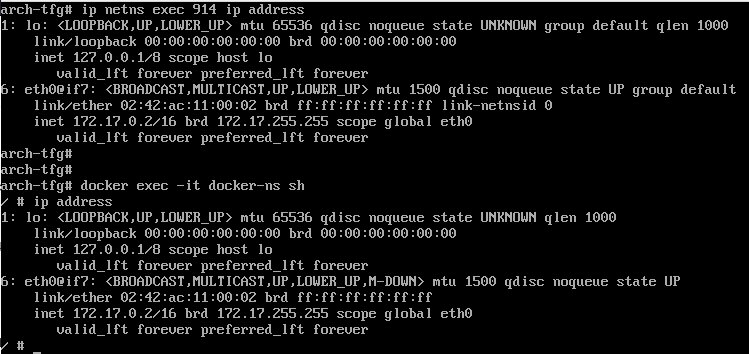
\includegraphics[width=1\textwidth]{img/docker_ns4.png}
			\caption{Comprobación de si un network namespaces pertenece a un contenedor Docker.}
			\label{img: comprobacion ns docker}
		\end{center}
	\end{figure}

	\begin{figure}[h!]
		\begin{center}
			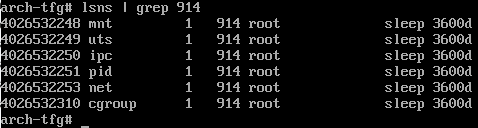
\includegraphics[width=0.75\textwidth]{img/docker_ns5.png}
			\caption{Namespaces asociados a un contenedor Docker.}
		\end{center}
	\end{figure}
	
	\pagebreak

	\section{Caso práctico: Virtualización para simulación de redes}
	\noindent En este apartado vamos a detallar los conceptos de virtualización de topologías de red para la evaluación y/o simulación de situaciones concretas de nuestras redes. Para ello, podemos modelar nuestros nodos de la red utilizando contenedores, siguiendo de esta manera el concepto de ``\textit{Virtual Network Function}'' que introdujimos en el segundo apartado de este documento. [\ref{sec: nfv}] \\
	
	\noindent Como bien hemos visto en el apartado anterior [\ref{sec: virt ligera y contenedores}], un contenedor es una abstracción de alto nivel de un sistema aislado, utilizando ``\textit{namespaces}''. Por lo tanto, tenemos varias maneras de enfocar el camino hacia el objetivo de modelar los nodos de nuestra red. Dichos caminos radican en que metodología de contenedores vamos a utilizar. Por ejemplo, algunos de los caminos a seguir podrían ser los siguientes:
	
	\begin{itemize}
		\item Crear un \textit{shell script} para desplegar los namespaces necesarios de nuestra topología, utilizando los comandos \texttt{nsenter} y \texttt{unshare}.
		\item Desplegar e interconectar contendores LXC, en el que cada contenedor cumpla una función dentro de nuestra topología (host, switch, controller...)
		\item Utilizar un simulador de red basado en ``namespaces'', dicho simulador se llama Mininet [\ref{bib: mininet home page}] y está creado en el lenguaje Python. El objetivo de este programa es el de crear una red virtual realista, utilizando un mismo kernel para todos los nodos de la red. Además, aporta las herramientas necesarias para interactuar con dicha topología.
	\end{itemize}
	
	\vspace{10px}
	
	%\noindent \textbf{\large Mininet}\\
	\subsection{\texttt{Mininet}: Simulador de redes}
	
	\noindent Profundizando en la última solución aportada, \texttt{mininet} [\ref{bib: mininet home page}], destacamos sus ventajas en la customización de topologías, además de la facilidad de compartir y desplegar dichas topologías en un hardware de uso general utilizando un único comando. Es por esto por lo que \texttt{mininet} es una herramienta muy útil para el desarrollo, la enseñanza y la investigación, siendo una herramienta muy determinante para la experimentación en el campo del \textit{Software Defined Networking} (SDN) ya que permite utilizar controladores basados en OpenFlow y P4.
	
	\subsubsection{Primeros pasos}
	\noindent Lo primero que tenemos que hacer para empezar a trabajar con este simulador, es proceder a su instalación. En la página web oficial, se nos detallan diferentes métodos para la instalación \href{http://mininet.org/download/}{Mininet: Download/Get Started with Mininet}, dichos métodos son: 
	
	\begin{itemize}
		\item Máquina virtual \texttt{Mininet}, todo previamente instalado.
		\item Instalación directamente del código fuente
		\item Instalación utilizando paquetes de una distribución.
	\end{itemize}

	\pagebreak

	\noindent La opción de utilizar una máquina virtual preconfigurada es mucho más rápida, ya que solo tendremos que descargar la última versión del enlace que encontramos en la web oficial del proyecto \href{https://github.com/mininet/mininet/releases/}{Github: mininet releases}. Una vez descargada, importamos dicha imagen en nuestro hipervisor, por ejemplo: \textit{VirtualBox}. Ejecutamos la máquina virtual recién importada y accedemos al sistema con el usuario: \texttt{mininet}/\texttt{mininet}. \\
	
	 \noindent Sin embargo, si deseamos realizar una instalación de \texttt{mininet} sobre nuestra distribución Linux. Podemos instalar el programa en función de la distribución que estemos usando:
	
	\begin{itemize}
		\item Debian/Ubuntu: \texttt{sudo apt-get install mininet}
		\item Fedora: \texttt{sudo dnf install mininet}
		\item openSUSE: \texttt{zypper in mininet}
		\item Arch Linux: \texttt{sudo pacman -S mininet}
	\end{itemize}

	\noindent Una vez instalado, podemos comprobar la versión ejecutando el siguiente comando en una terminal:
	\begin{verbatim}
		$ mn --version
	\end{verbatim}

	\noindent Por otro lado, Mininet permite utilizar diferentes switches y controladores para sus topologías. Para esta explicación, vamos a utilizar Open vSwitch [\ref{bib: open vswitch}] como controlador, en el modo \textit{bridge/standalone}. Si queremos comprobar que Open vSwitch está instalado correctamente para mininet, podemos ejecutar el siguiente comando en una terminal:
	\begin{verbatim}
		$ mn --switch ovsbr --test pingall
	\end{verbatim}

	\noindent En el caso de que el comando anterior nos de un error, tendremos que instalar Open vSwitch para nuestra distribución y asegurarnos de que el servicio esté funcionando. Para iniciar el servicio de Open vSwitch, tendremos que hacer lo siguiente:
	\begin{verbatim}
		$ sudo systemctl start openvswitch.service
	\end{verbatim}

	\noindent En el caso de Arch Linux, sería tal que así:
	\begin{verbatim}
		$ sudo systemctl start ovs-vswitchd.service
	\end{verbatim}

	%% Ruta miniedit:
	% /usr/lib/python3.10/site-packages/mininet/examples/miniedit.py
	
	\pagebreak
	
	%\subsubsection{Implementación topología simple}
	\subsubsection{Ejemplos}
	
	\noindent \textbf{Topología simple}\\
	
	\noindent En este apartado, vamos a trabajar la dualidad entre implementar una topología utilizando únicamente namespaces, a implementar esa misma topología utilizando mininet. Para ello, vamos a trabajar con una red formada por dos hosts, conectados entre sí mediante un conmutador de paquetes (\textit{switch}), que será manejado por un controlador. \\
	
	\begin{figure}[h!]
		\begin{center}
			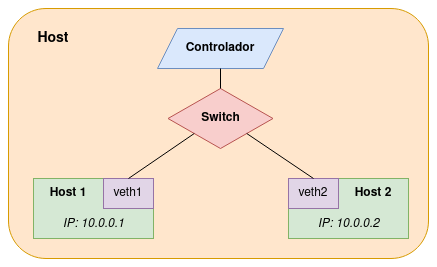
\includegraphics[width=0.6\textwidth]{img/ns_mn_single.png}
			\caption{Diagrama de la topología simple a implementar.}
		\end{center}
	\end{figure}
	
	\noindent \textbf{\large Ejemplo: topología simple sin usar \texttt{mininet}}\\
	
	\noindent Primero, accedemos a nuestra máquina Host, en la que desplegaremos los namespaces asociados a la topología. Una vez estamos dentro de la cuenta \texttt{root}, procedemos a crear los \texttt{network namespaces} de cada host. 
	
	\begin{verbatim}
$ ip netns add host-1
$ ip netns add host-2
	\end{verbatim}

	\noindent Con los \texttt{network namespaces} ya creados, lo siguiente es crear el conmutador de paquetes. En este caso, vamos a utilizar \textit{Open vSwitch} [\ref{bib: open vswitch}], que previamente hemos instalado en conjunto con mininet. Para crear dicho switch, ejecutamos el siguiente comando:
	
	\begin{verbatim}
$ ovs-vsctl add-br switch-1
	\end{verbatim}

	\noindent Para interconectar los hosts con el conmutador, utilizaremos interfaces de red virtuales de tipo pares de ethernet (\texttt{veth pairs}) (explicados en [\ref{sec: veth}]). Por eso mismo, utilizamos los siguientes comando para establecer los enlaces punto a punto:
	
	\begin{verbatim}
$ ip link add host-1-veth1 type veth peer name switch-1-veth1
$ ip link add host-2-veth2 type veth peer name switch-1-veth2
	\end{verbatim}

	\pagebreak

	\noindent En este punto, tendremos que asociar las interfaces a los \texttt{network namespaces}.
	
	\begin{verbatim}
$ ip link set host-1-veth1 netns host-1
$ ip link set host-2-veth2 netns host-2
	\end{verbatim}

	\noindent Por otro lado, también será necesario que añadamos el otro extremo de las interfaces al switch.
	
	\begin{verbatim}
$ ovs-vsctl add-port switch-1 switch-1-veth1
$ ovs-vsctl add-port switch-1 switch-1-veth2
	\end{verbatim}

	\noindent Ahora es el momento de configurar el switch para que funcione como un conmutador. Para ello, utilizamos el controlador Open vSwitch (tal y como pudimos ver en los ejemplos asociados a pares ethernet [\ref{sec: veth}]). Por lo tanto, para hacerlo funcionar en nuestra topología, tendremos que ejecutar los siguientes comandos:
	
	\begin{verbatim}
$ ovs-vsctl set-controller switch-1 tcp:127.0.0.1
$ ovs-testcontroller ptcp: &
	\end{verbatim}

	\noindent Si queremos comprobar que hemos creado correctamente el switch virtual, podemos utilizar el siguiente comando:
	
	\begin{verbatim}
$ ovs-vsctl show
	\end{verbatim}
	
	\begin{figure}[h!]
		\begin{center}
			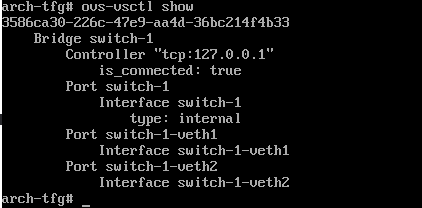
\includegraphics[width=0.6\textwidth]{img/ns_single_1.png}
			\caption{Captura de la configuración del switch usando Open vSwitch.}
		\end{center}
	\end{figure}
	
	\noindent Una vez tenemos todos los dispositivos configurados, lo que tendremos que hacer es asignar direcciones IP a cada host, y pondremos en funcionamiento las interfaces asociadas.
	
	\begin{verbatim}
$ ip netns exec host-1 ip addr add 10.0.0.1/24 dev host-1-veth1
$ ip netns exec host-2 ip addr add 10.0.0.2/24 dev host-2-veth2
$ ip netns exec host-1 ip link set host-1-veth1 up
$ ip netns exec host-1 ip link set lo up
$ ip netns exec host-2 ip link set host-2-veth2 up
$ ip netns exec host-2 ip link set lo up
$ ip link set switch-1-veth1 up
$ ip link set switch-1-veth2 up
	\end{verbatim}

	\pagebreak

	\noindent En este punto, ya deberíamos tener conectividad entre ambos hosts. Para ello, lo que podemos hacer es realizar un ping entre \texttt{host-1} (IP: 10.0.0.1) y \texttt{host-2} (IP: 10.0.0.2).
	
	\begin{verbatim}
$ ip netns exec host-1 ping 10.0.0.2
	\end{verbatim}

	\begin{figure}[h!]
		\begin{center}
			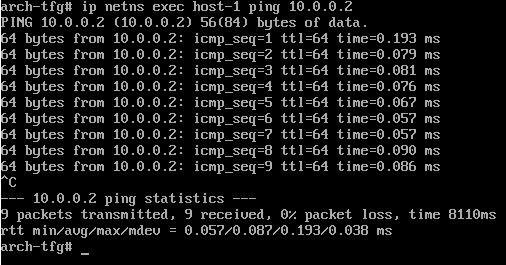
\includegraphics[width=0.65\textwidth]{img/ns_single_2.png}
			\caption{Ejecución ping entre \texttt{host1} y \texttt{host2}.}
		\end{center}
	\end{figure}
	
	\vspace{10px}
	%\pagebreak
	
	\noindent \textbf{\large Ejemplo: topología simple utilizando \texttt{mininet}}\\
	
	\noindent En este caso, vamos a replicar la misma topología del ejemplo anterior, pero esta vez utilizando mininet. Dado que es una topología sencilla, podemos ejecutarla con un único comando. 
	
	\begin{verbatim}
$ mn --topo single,2 --controller=ovsc
	\end{verbatim}

	\begin{figure}[h!]
		\begin{center}
			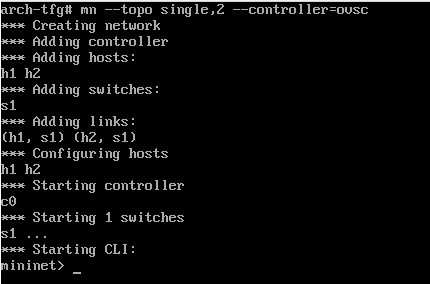
\includegraphics[width=0.55\textwidth]{img/mn_single_1.png}
			\caption{Ejecución topología simple en \texttt{mininet}.}
		\end{center}
	\end{figure}

	\pagebreak
	
	\noindent Como podemos comprobar en la captura anterior, una vez ejecutamos el comando, la topología se crea automáticamente. Si quisiéramos comprobar la conectividad entre los diferentes hosts, solo tendríamos que ejecutar el siguiente comando dentro de la terminal de mininet.
	
	\begin{verbatim}
mininet> h1 ping h2
	\end{verbatim}

	\begin{figure}[h!]
		\begin{center}
			\includegraphics[width=0.65\textwidth]{img/mn_single_2.png}
			\caption{Ping entre hosts de topología simple en \texttt{mininet}.}
			\label{img: ping mn simple}
		\end{center}
	\end{figure}

	%\pagebreak
	
	\noindent Mientras tenemos activa la topología de mininet, podemos comprobar qué namespaces ha creado para dicha topología. 
	
	\begin{figure}[h!]
		\begin{center}
			\includegraphics[width=0.8\textwidth]{img/mn_single_3.png}
			\caption{Comprobación de namespaces utilizados por topología en \texttt{mininet}.}
			\label{img: lsns mininet 1}	
		\end{center}
	\end{figure}

	\noindent Como bien podemos ver en la imagen (\ref{img: lsns mininet 1}), \texttt{mininet} solo está utilizando los namespaces \texttt{mount} y \texttt{network} para el despliegue de la topología. \\
	
	\noindent Si quisiéramos implementar esta topología simple utilizando la API Python que está incluida en \texttt{mininet}, podemos ejecutar el código del Anexo 4 [\ref{sec: anexo 4}] (ver código \ref{lst: topo simple})
	
	\pagebreak
	
	\noindent Ejecutando el código implementado, podemos comprobar como al iniciar la topología se realizan comprobaciones tanto de conectividad, utilizando \texttt{ping}, como de velocidades, utilizando \texttt{iperf}. En la figura \ref{img: iperf mn simple} podemos comprobar cual es el rendimiento de los enlaces al ejecutar dicha topología.
	
	\begin{figure}[h!]
		\begin{center}
			\includegraphics[width=0.8\textwidth]{img/mn_single_4.png}
			\caption{Ejecución de \texttt{iperf} sobre topología simple en \texttt{mininet}.}
			\label{img: iperf mn simple}	
		\end{center}
	\end{figure}
	
	
	\noindent \textbf{\large Ejemplo: limitación de recursos usando \texttt{mininet}}\\
	
	\noindent En este ejemplo, vamos a profundizar sobre como aplicar limitaciones de recursos a una topología desplegada con \texttt{mininet}. Algunos de los recursos más importantes a tener en cuenta, son los siguientes:
	
	\begin{itemize}
		\item \textit{CPU}. Nos permite asignar el máximo uso de CPU de un dispositivo de la tecnología. Esto nos permitirá ajustar nuestra simulación a un entorno más real, además de permitirnos gestionar más los recursos disponibles.
		\item \textit{Latencia}. Permite establecer una latencia máxima a un enlace entre dispositivos.
		\item \textit{Ancho de banda}. Permite establecer un máximo de ancho de banda para un enlace entre dispositivos.
	\end{itemize}
	
	\noindent Por lo tanto, a modo de ejemplo, vamos a utilizar la topología anterior, pero aplicando una limitación de ancho de banda, latencia y CPU a uno de los enlaces que conectan un host con el switch. El código utilizado para este ejemplo lo podemos encontrar en el Anexo 4 [\ref{sec: anexo 4}] (ver código \ref{lst: topo simple cpu mn}).
	
	\noindent Para ejecutar la topología, utilizamos el siguiente comando:
	\begin{verbatim}
sudo python limit.py	
	\end{verbatim}

	\noindent Como podemos comprobar en la figura \ref{img: mn limit 1}, al ejecutar la topología, vemos como en consola nos aparece un aviso de que se ha limitado un enlace a 5 Mbit de ancho de banda y 80 ms de latencia. Por otro lado, una vez la topología esta funcionando, se procede a una comprobación de conectividad entre ambos host, seguidamente, se ejecuta la herramienta \texttt{iperf} para comprobar cual es el ancho de banda máximo entre ambos hosts.
	
	\pagebreak
	
	\begin{figure}[h!]
		\begin{center}
			\includegraphics[width=0.75\textwidth]{img/mn_limit_1.png}
			\caption{Ejecución topología simple limitada en \texttt{mininet}. (1/2)}
			\label{img: mn limit 1}	
		\end{center}
	\end{figure}

	\noindent Comparando los resultados obtenidos entre la topología sin limitar (ver figura \ref{img: iperf mn simple}) y la topología limitada tanto en CPU como en los enlaces (ver figura \ref{img: mn limit 1}), podemos comprobar que efectivamente el ancho de banda que obtenemos de la herramienta \texttt{iperf} se ve claramente reducido, pasando de 20 Gbits/sec a 4.58 Mbits/sec. Por lo tanto, podemos concluir que efectivamente se están aplicando correctamente la limitación de ancho de banda. \\
	
	\noindent Por otro lado, otra medida interesante a comparar es el tiempo que tarda un paquete entre que es enviado a un host y la respuesta vuelve al host emisor. Esto lo podemos comprobar con la herramienta \texttt{ping}. Dado que hemos fijado la latencia de uno de los enlaces (fijado a 80 ms), deberíamos obtener un valor del campo \texttt{time} mayor que al que obtenemos en la topología simple sin limitar. Ver figura \ref{img: mn limit 2}.
	
	\begin{figure}[h!]
		\begin{center}
			\includegraphics[width=0.65\textwidth]{img/mn_limit_2.png}
			\caption{Ejecución topología simple limitada en \texttt{mininet}. (2/2)}
			\label{img: mn limit 2}	
		\end{center}
	\end{figure}

	\noindent Al igual que para el ancho de banda, los resultados de la topología sin limitar (ver figura \ref{img: ping mn simple}) y la topología limitada (ver figura \ref{img: mn limit 2}), son totalmente diferentes. Estas limitaciones son muy interesantes para modelar una topología con características lo más cercanas a un despliegue real. Por lo tanto, para simular una red, deberemos configurar estos valores de ancho de banda y latencia para cada uno de los enlaces de la topología.
	
	\pagebreak
	
	\noindent \textbf{\large Ejemplo: controlador externo}\\
	
	\noindent En los ejemplos anteriores de \texttt{mininet}, hemos estado utilizando el controlador OpenFlow ``built in'' de \texttt{mininet}, es decir, hemos utilizado \texttt{Open vSwitch} como controlador de los dispositivos de red de nuestra topología (switches). Dicho controlador, tiene como tarea distribuir, de manera dinámica y según ciertas reglas, la información asociada al encaminamiento de los paquetes de la red, rellenando las \texttt{flow-table} de los switches. \\
	
	\noindent Sin embargo, \texttt{mininet} nos permite la utilización de otros controladores SDN externos, que además pueden estar basados en las diferentes versiones del protocolo OpenFlow que están disponibles actualmente, permitiendo así compatibilidad con más dispositivos físicos disponibles en el mercado. \\
	
	\noindent Algunos de los controladores SDN que más se utilizan actualmente son los siguientes:
	\begin{itemize}
		\item \texttt{OpenDayLight} [\ref{bib: opendaylight}]. Controlador SDN más utilizado. Desarrollado en el lenguaje Java. Filosofía modular, permite desarrollar aplicaciones sobre el, de modo que podamos customizar y automatizar las redes a la escala que queramos.
		
		\item \texttt{POX}/\texttt{NOX} [\ref{bib: pox}][\ref{bib: nox}]. Controlador SDN escrito en Python/C++. Soporta OpenFlow 1.0. Permite un desarrollo rápido y asíncrono.
		
		\item \texttt{Ryu} [\ref{bib: ryu}]. Controlador SDN escrito en Python. Filosofía basada en componentes, por lo que permite una fácil integración con nuevas aplicaciones. Aporta una \texttt{northbound API} bien definida. Soporta OpenFlow 1.0, 1.2, 1.3, 1.4 y 1.5, además de otros protocolos como Netconf.
				
		\item \texttt{ONOS} [\ref{bib: onos}]. Controlador SDN muy utilizado. Desarrollado en el lenguaje Java y que tiene una arquitectura modular. 
	\end{itemize}

	\vspace{20px}
	\noindent \textbf{Controlador \texttt{Ryu}}\\

	\noindent A modo de ejemplo, vamos a instalar y ejecutar una topología en \texttt{mininet} utilizando el controlador SDN \texttt{Ryu}.  \\
	
	\noindent Lo primero, para instalar \texttt{Ryu} tenemos que ejecutar el comando siguiente. Para este ejemplo, vamos a utilizar la misma máquina virtual que estamos utilizando para \texttt{mininet}.
	
	\begin{verbatim}
$ git clone https://github.com/faucetsdn/ryu.git
$ pip install ryu/.
	\end{verbatim}

	\noindent En una terminal (la llamaremos terminal A), ejecutaremos una topología de \texttt{mininet}. Por ejemplo, utilizando el siguiente comando:
	\begin{verbatim}
$ sudo mn --topo tree,depth=3 --mac --switch ovsk --controller remote
	\end{verbatim}

	\noindent Con dicha topología, estaremos simulando una red de tipo árbol con 8 hosts, 7 switchs \texttt{Open vSwitch} y un controlador remoto (escuchando en la dirección \texttt{127.0.0.1:6653}). 
	
	\pagebreak
	
	\noindent Una vez ejecutada la topología, podemos comprobar que no tenemos conectividad entre los host utilizando el comando \texttt{pingall}, esto es debido a que no tenemos ejecutando nuestro controlador. (ver Figura \ref{img: mn ryu 1})
	
	\begin{figure}[h!]
		\begin{center}
			\includegraphics[width=1\textwidth]{img/mn_ryu_1.png}
			\caption{Ejecución topologia \texttt{mininet} sin controlador asignado (terminal A)}
			\label{img: mn ryu 1}	
		\end{center}
	\end{figure}
	
	\noindent En este caso, vamos a ejecutar nuestro controlador con una configuración de switch que soporta OpenFlow 1.3 (alojado en \texttt{simple\_switch\_13.py}). Para ello, ejecutamos el siguiente comando en una terminal diferente a la terminal A (la llamaremos terminal B).
	
	\begin{verbatim}
$ ryu run ryu.app.simple_switch_13
	\end{verbatim}
	
	\noindent Una vez ejecutado, nos aparecerá en la terminal B la información acerca de los módulos que \texttt{Ryu} ha cargado para dar la funcionalidad que deseamos. Además, en dicha terminal se irán mostrando los diferentes paquetes que conmute el switch. \\
	
	\noindent Si ahora comprobamos la conectividad en la topología de \texttt{mininet} (escribiendo en la terminal A el comando \texttt{pingall}), podemos ver como efectivamente ahora si que los paquetes llegan a su destino. Por lo tanto, podemos determinar que efectivamente el controlador SDN está rellenando correctamente la \texttt{flow-table} del switch. (ver Figura \ref{img: mn ryu 2}) 
	
	\pagebreak
	
	\begin{figure}[h!]
		\begin{center}
			\includegraphics[width=0.7\textwidth]{img/mn_ryu_2.png}
			\caption{Ejecución del controlador \texttt{Ryu} (terminal inferior, B) y posterior \texttt{pingall} en \texttt{mininet} (terminal superior, A)}
			\label{img: mn ryu 2}	
		\end{center}
	\end{figure}
	
	\noindent Por otro lado, otra funcionalidad interesante de este controlador es el visualizador de topologías. Nos permite ver en una página web la topología de nuestra red, es decir, como se interconectan los diferentes switches de la red. Para ello, solo tenemos que ejecutar el siguiente comando en la terminal B (si tenemos activo el ejemplo de \texttt{simple\_switch\_13.py}, pararemos su ejecución con Ctrl+C):
	\begin{verbatim}
$ ryu run --observe-links ryu.app.simple_switch_13 ryu.app.gui_
topology.gui_topology
	\end{verbatim}

	\pagebreak

	\noindent Ahora, una vez ejecutado el comando anterior, tenemos que utilizar un navegador web y dirigirnos a la siguiente dirección: \url{http://localhost:8080/}. Después de acceder a dicha página, podemos ver como se nos presenta la topología de la red que estamos controlando (ver Figura \ref{img: mn ryu 3}). [\ref{bib: ryu gui}]
	
	%\pagebreak
	\vspace{10px}
	
	\begin{figure}[h!]
		\begin{center}
			\includegraphics[width=1\textwidth]{img/mn_ryu_3.png}
			\caption{Herramienta \textit{Topology Viewer} del controlador \texttt{Ryu}}
			\label{img: mn ryu 3}	
		\end{center}
	\end{figure}
	
	\pagebreak
	
	\subsection{\texttt{Containernet}: Simulador de redes}
	
	\noindent Por otro lado, existen otras implementaciones de simuladores que extienden la funcionalidad de \texttt{mininet}, permitiendo abarcar muchas más situaciones a simular. A modo de ejemplo, destacamos \texttt{containernet} [\ref{bib: containernet github}], siendo un simulador de red basado en \texttt{mininet} que permite utilizar contenedores de \texttt{Docker} como hosts en una red emulada. Esta funcionalidad permite construir entornos de simulación para redes de tipo \textit{cloud}. \\
	
	\noindent Además, es un proyecto muy activo por la comunidad investigadora, ya que permite evaluar topologias de \textit{cloud computing}, \textit{network function virtualization} (NFV) o \textit{multi-access edge computing} (MEC). Un ejemplo de esto es el emulador \href{https://github.com/containernet/vim-emu}{vim-emu: A NFV multi-PoP emulation Platform}, desarrollado por \href{https://www.sonata-nfv.eu/}{SONATA project}, y que está basado en \texttt{containernet}.
	
	\begin{figure}[h!]
		\begin{center}
			\includegraphics[width=0.3\textwidth]{img/containernet_logo.png}
			\caption{Logotipo del projecto \texttt{containernet} [\ref{bib_img: containernet logo}]}	
		\end{center}
	\end{figure}

	\vspace{10px}
	
	\noindent \textbf{\large Características}\\
	
	\noindent Algunas de las características más importantes que nos aporta \texttt{containernet}, son las siguientes:
	
	\begin{itemize}
		\item Añadir y eliminar contenedores \texttt{Docker} a topologias de \texttt{mininet}. Interconectar dichos contenedores con la topología.
		
		\item Ejecutar comandos dentro de los contenedores, utilizando \texttt{mininet CLI}.
		
		\item Cambios dinámicos en las topologías. Permite añadir o eliminar contenedores a topologias que estén en ejecución.
		
		\item Limitar recursos de los contenedores \texttt{Docker}, de forma individual.
		
		\item Permite configurar los enlaces en base a: \textit{delay}, \textit{bandwidth}, \textit{loss} o \textit{jitter}.
	\end{itemize}
	
	\pagebreak
	
	\subsubsection{Primeros pasos}
	\noindent Lo primero que tenemos que hacer para trabajar con este simulador es proceder a su instalación. Para ello, nos vamos a guiar por los pasos que están detallados en la documentación del proyecto en \href{https://containernet.github.io/#installation}{Github: containernet}. Lo primero que podemos comprobar es que se nos aportan dos opciones de instalación:
	\begin{itemize}
		\item ``Bare-metal installation''. Hace referencia a una instalación sobre la distribución Ubuntu 20.04 LTS con Python3.
		
		\item ``Nested Docker deployment''. Utiliza un contenedor Docker con privilegios para desplegar en su interior otro entorno Docker en el que ejecutar las topologias de \texttt{containernet}. Esta opción tiene deshabilitado la característica de limitación de recursos.
	\end{itemize}

	\noindent Para nuestro entorno de pruebas, hemos elegido instalar \texttt{containernet} en una máquina virtual en \textit{VirtualBox}, utilizando Ubuntu 20.04 LTS, tal y como leemos en su documentación. Para ello, seguimos las instrucciones tal que:
	
	\begin{enumerate}
		\item Instalación de \texttt{Ansible}
		\begin{verbatim}
$ sudo apt-get install ansible
		\end{verbatim}
	
		\item Clonamos el repositorio de Github:
		\begin{verbatim}
$ git clone https://github.com/containernet/containernet.git
		\end{verbatim}
	
		\item Ejecutamos el ``playbook'' de \texttt{Ansible}, el cual instalará todas las dependencias y posteriormente \texttt{containernet}.
		\begin{verbatim}
$ sudo ansible-playbook -i "localhost," -c local containernet/
ansible/install.yml
		\end{verbatim}
	
		\begin{figure}[h!]
			\begin{center}
				\includegraphics[width=0.75\textwidth]{img/cn_install1.png}
				\caption{Instalación \texttt{containernet} en Ubuntu 20.04 LTS (1/2)}	
			\end{center}
		\end{figure}
	\end{enumerate}
	
	\pagebreak
	
	\begin{figure}[h!]
		\begin{center}
			\includegraphics[width=0.75\textwidth]{img/cn_install2.png}
			\caption{Instalación \texttt{containernet} en Ubuntu 20.04 LTS (2/2)}
			\label{img: containernet install}
		\end{center}
	\end{figure}
	
	\noindent Si la instalación es satisfactoria, la salida de la consola debería ser muy similar a la que vemos en la imagen \ref{img: containernet install}. Al final de la ejecución del ``playbook'' de \texttt{Ansible}, se nos muestra un resumen de las tareas ejecutadas, y cuales de ellas se han realizado correctamente, o bien, cuales han dado error al ejecutarse. En nuestro caso, se ha instalado correctamente.
	
	\subsubsection{Implementación topología simple}
	\noindent En este apartado vamos a comentar como desplegar una topología simple dentro de \texttt{containernet}. Dado que la filosofía de este programa es extender la funcionalidad de \texttt{mininet} hacia la posibilidad de que los hosts sean contenedores de Docker, lo que tendremos como topología son varios contenedores Docker, interconectados cada uno con un switch. Como podemos ver, el diagrama de la red es muy parecido al que utilizamos como topología simple en \texttt{mininet}.
	
	\begin{figure}[h!]
		\begin{center}
			\includegraphics[width=0.6\textwidth]{img/cn_simple_diag.png}
			\caption{Diagrama topología simple utilizando \texttt{containernet}}
		\end{center}
	\end{figure}

	\pagebreak
	
	\noindent Esta topología que podemos ver en el diagrama, está ubicada en la carpeta de \texttt{examples} dentro de \texttt{containernet}. Con esta topología podemos ver las bases del simulador, y comprobar como puede trabajar con las características de \texttt{mininet}, a la vez de implementar los hosts como contenedores Docker. El código Python utilizado para ejecutar el ejemplo lo encontramos en el Anexo 4 [\ref{sec: anexo 4}] (ver código \ref{lst: topo simple containernet}). \\
	
	\noindent Para ejecutar el ejemplo, tendremos que lanzar el siguiente comando:
	\begin{verbatim}
$ sudo python3 containernet_example.py
	\end{verbatim}

	\noindent La salida por consola será muy similar a la que obtendríamos en \texttt{mininet}, sin embargo, podemos comprobar como aparece la información respectiva de nuestros contenedores Docker que van a tener la función de host en la topología. Todo esto lo podemos ver en la figura \ref{img: cn simple 1}.
	
	\begin{figure}[h!]
		\begin{center}
			\includegraphics[width=1\textwidth]{img/cn_example1.png}
			\caption{Ejecución de topología simple en \texttt{containernet} (1/5)}
			\label{img: cn simple 1}
		\end{center}
	\end{figure}

	\noindent Una vez se termina de ejecutar la topología, nos deja activa la \texttt{CLI} para que podamos interactuar con la misma. En nuestro caso, vamos a comprobar cual es la configuración de red asociada al host 1, para ver como ha gestionado las interfaces del contenedor de Docker. Para ello, ejecutamos el siguiente comando:
	\begin{verbatim}
containernet> d1 ifconfig
	\end{verbatim}

	\noindent Como podemos comprobar en la figura \ref{img: cn simple 2}, el host 1 tiene una interfaz (\texttt{d1-eth0}) que es la que estará en uso para nuestra topología de \texttt{containernet}, además dispone de otra interfaz (\texttt{eth0}) que será la que utilice para comunicarse con el controlador de Docker. Por lo tanto, podemos ver como \texttt{containernet} no manda su tráfico por el \texttt{bridge} que crea Docker, sino que añade una interfaz específica (un extremo de un par ethernet virtual, \textit{veth}) por el que encaminará el tráfico de la simulación.

	\pagebreak

	\begin{figure}[h!]
		\begin{center}
			\includegraphics[width=0.55\textwidth]{img/cn_example2.png}
			\caption{Ejecución de topología simple en \texttt{containernet} (2/5)}
			\label{img: cn simple 2}
		\end{center}
	\end{figure}

	\noindent Por otro lado, mientras tenemos la topología ejecutandose, podemos comprobar como aparecen los contendores Docker en nuestro sistema. Además, también podemos acceder a una \textit{shell} de uno de los contendores (hosts de \texttt{containernet}) y comprobar que efectivamente el resultado es el mismo que si accedemos desde la \texttt{CLI} de \texttt{containernet}. Para ello, hemos comprobado la configuración de red del mismo host que vimos en la figura \ref{img: cn simple 2}, esto lo podemos ver en la figura \ref{img: cn simple 3}

	\begin{figure}[h!]
		\begin{center}
			\includegraphics[width=0.85\textwidth]{img/cn_example3.png}
			\caption{Ejecución de topología simple en \texttt{containernet} (3/5)}
			\label{img: cn simple 3}
		\end{center}
	\end{figure}

	\pagebreak

	\noindent Al igual que hacíamos en \texttt{mininet}, podemos comprobar conectividad entre dos hosts utilizando el comando \texttt{ping}, para ello podemos ejecutar en la \texttt{CLI} el siguiente comando:
	\begin{verbatim}
containernet> d1 ping -c4 d2
	\end{verbatim}

	\noindent Una vez ejecutado, observamos como la salida nos muestra el \texttt{ping} que se ha ejecutado, y como efectivamente hay conectividad entre los dos hosts. Este resultado lo podemos ver en la figura \ref{img: cn simple 4}.

	\begin{figure}[h!]
		\begin{center}
			\includegraphics[width=1\textwidth]{img/cn_example4.png}
			\caption{Ejecución de topología simple en \texttt{containernet} (4/5)}
			\label{img: cn simple 4}
		\end{center}
	\end{figure}

	\noindent Por último, si ya no queremos seguir ejecutando la topología, tendremos que ejecutar el comando \texttt{exit}. Este comando nos permitirá revertir la configuración asociada a la topología, además de apagar y eliminar los contenedores Docker que estaban ejerciendo como hosts. El resultado de la ejecución de este comando lo podemos ver en la figura \ref{img: cn simple 5}.

	\pagebreak

	\begin{figure}[h!]
		\begin{center}
			\includegraphics[width=0.5\textwidth]{img/cn_example5.png}
			\caption{Ejecución de topología simple en \texttt{containernet} (5/5)}
			\label{img: cn simple 5}
		\end{center}
	\end{figure}
	
	%\subsection{Interconexión física de diferentes red virtuales}
	%\subsection{Evaluación de prestaciones}
	
	\pagebreak
	
	\section{Conclusiones y propuestas futuras}
	
	\noindent En este capítulo vamos a comentar las conclusiones obtenidas al realizar el presente trabajo. \\
	
	\noindent En primer lugar, hemos presentado la problemática actual de la escalabilidad de las redes y como se está trabajando para un futuro basado en el software y en la descentralización. Esto supone una búsqueda para poder alejarnos de hardware específico/embebido, para acércanos a un hardware de carácter general en el que podamos desplegar nuestros servicios, todo esto, potenciado con la virtualización de los sistemas. A raíz de esto, hemos definido \texttt{NFV} y los conceptos más importantes para entender que és y por qué es un desarrollo muy importante para las telecomunicaciones. Además, lo hemos ``diferenciado'' respecto al concepto de \texttt{SDN}, y comprobado como ambas son tecnologías que van a ir de la mano, ya que una depende de la otra. \\
	
	\noindent Por otro lado, se ha explicado las diferentes interfaces de red virtuales de Linux, ya que son realmente importantes para las soluciones de virtualización. Para completar la explicación, se ha seguido una metodología basada en ejemplos, por lo que hemos podido comprobar la funcionalidad y el objetivo de cada una de las interfaces expuestas. Hemos comprobado la importancia de interfaces como pueden ser los pares ethernet o bien los tup/tap, aunque sobre todo tap. \\
	
	\noindent En el sentido de \texttt{namespaces}, se han definido los namespaces presentes dentro del Kernel de Linux. Se ha verificado el potencial que posee esta tecnología, y como está muy presente en diferentes tecnologías que están fuertemente arraigadas por la comunidad, por ejemplo \texttt{LXC} o \texttt{Docker}. Gracias a los ejemplos, se ha podido comprender fácilmente el funcionamiento de cada uno de los namespaces. \\
	
	\noindent En el punto de virtualización ligera, hemos aprendido que implementaciones software tenemos disponibles para realizar virtualización ligera. Además, hemos recreado un contenedor paso a paso, de modo que hemos podido comprobar la importancia de los namespaces. Por otro lado, con las definiciones de \texttt{LXC} y de \texttt{Docker}, hemos iniciado al uso de ambas herramientas, facilitando su posterior uso. \\
	
	\noindent Por último, se han propuesto ciertas herramientas que utilizan la virtualización ligera para simular redes de comunicaciones. En este caso hemos hablado de \texttt{mininet}, como una implementación basada totalmente en namespaces, y de \texttt{containernet} como un ``fork'' de \texttt{mininet} que está extendido para trabajar con hosts de Docker. Ambas herramientas son muy importantes ya que permiten crear entornos de desarrollo e investigación para el área de \texttt{SDN}. Nos permite realizar pruebas con topologías de gran tamaño de manera sencilla y rápida. \\
	
	\noindent En resumen, podemos concluir que el presente trabajo ha cumplido todos los objetivos propuestos, ya que se ha profundizado sobre la virtualización ligera, y se ha ido construyendo una ``guía'' a base de explicaciones y ejemplos, que nos permite comprender los entresijos de simuladores de redes basados en dicha virtualización, como puede ser \texttt{mininet}. \\
	
	\pagebreak
	
	%\subsection{Propuestas futuras}
	\noindent \textbf{\large Propuestas futuras}\\
	
	\noindent Algunas de las líneas de investigación que pueden resultar interesantes para continuar este proyecto, son las siguientes:
	\begin{itemize}
		\item Profundizar en las diferencias de rendimiento entre utilizar una virtualización ``dura'', usando un hipervisor (por ejemplo VirtualBox), respecto a una solución basada en contenedores, como las que hemos comentado en este trabajo. Por otro lado, en temas de rendimiento, también se podría estudiar cual podría ser el límite en la simulación de redes utilizando virtualización ligera.
		
		\item Investigar sobre modificaciones del protocolo \texttt{OpenFlow}, como puede ser \url{https://github.com/Orange-OpenSource/oko}, que nos permite aplicar programas con los que filtrar paquetes de la red utilizando \texttt{BPF} (\textit{Berkley Packet Filter}). Por otro lado, sería realmente importante investigar la tecnología \texttt{DPDK}, ya que nos permite acceder directamente a la información de nuestras interfaces de red, además de mejorar considerablemente el \textit{throughput} en comparación de si utilizamos un \textit{Linux bridge}.
		
		\item Estudiar el lenguaje de programación \texttt{P4} (\url{https://p4.org/}), ya que ahora mismo esta siendo muy importante para el desarrollo de soluciones software en routers y switches. Se esta observando gran aceptación por la comunidad investigadora, y hay un creciente interés para su implantación. El objetivo de este lenguaje de programación es el de controlar el flujo de los paquetes de datos entre los diferentes planos de información que maneja el dispositivo. A diferencia de otros lenguajes de programación, como C o C++, \texttt{P4} está definido teniendo en mente que tiene que ser específico para las redes, por lo que presenta ciertas construcciones específicas para optimizar el flujo de la información.
	\end{itemize}

	%%% Bibliography
	\pagebreak
	\section{Bibliografía}
	%\addcontentsline{toc}{section}{Bibliografía}
	
	\subsection*{Enlaces y referencias}
	\addcontentsline{toc}{subsection}{Enlaces y referencias}
	%%\hyperref[bib:link1]{\emph{Reference of bibliography}}
	\begin{enumerate}
		%1
		\item 
		\label{bib:ns overview} \href{https://lwn.net/Articles/531114/}{\textit{Namespaces}}
		
		%2
		\item 
		\label{bib:ns tutorial1} \href{https://laurel.datsi.fi.upm.es/~ssoo/SOA/namespaces.html}{Tutorial: Espacio de nombres en Linux}
		
		%3
		\item 
		\label{bib:time ns} \href{https://www.phoronix.com/scan.php?page=news_item&px=Linux-Time-Namespace-Coming}{\textit{Time namespaces coming to linux}}
		
		%4
		\item 
		\label{bib:container is a lie} \href{https://platform.sh/blog/2020/the-container-is-a-lie/}{\textit{Container is a lie. Namespaces}}
		
		%5
		\item 
		\label{bib:link5} \href{https://locurastecnicas.blogspot.com/2020/09/linux-namespaces-y-cgroups.html}{\textit{Namespaces.} Uso de \textit{cgroups}.}
		
		%6
		\item 
		\label{bib:link6} \href{https://www.youtube.com/watch?v=_WgUwUf1d34}{\textit{Introduction to Network Namespaces}}
		
		
		%7
		\item
		\label{bib: mount namespace redhat} \href{https://www.redhat.com/sysadmin/mount-namespaces}{\textit{Build a container by hand: the mount namespace}}
		
		
		%8
		\item
		\label{bib:pid wikipedia}
		\href{https://en.wikipedia.org/wiki/Process_identifier}{Indentificador de procesos (\textit{process id})}
		
		
		%9
		\item
		\label{bib:link9}
		\href{https://www.redhat.com/sysadmin/linux-pid-namespaces}{\textit{Linux PID namespaces work with containers}}
		
		%10
		\item
		\label{bib:link10}
		\href{https://blogs.igalia.com/dpino/2016/04/10/network-namespaces/}{\textit{Network Namespaces}}
		
		%11
		\item
		\label{bib:virtual interface list}
		\href{https://developers.redhat.com/blog/2018/10/22/introduction-to-linux-interfaces-for-virtual-networking#veth}{\textit{Introduction to Linux interfaces for virtual networking}}
		
		
		%12
		\item
		\label{bib:link12}
		\href{https://elpuig.xeill.net/Members/vcarceler/articulos/introduccion-a-los-grupos-de-control-cgroups-de-linux}{\textit{Introducción a los grupos de control (cgroups) de Linux}}
		
		%13
		\item
		\label{bib:time ns kernel}
		\href{https://git.kernel.org/pub/scm/linux/kernel/git/tip/tip.git/commit/?h=timers/core&id=769071ac9f20b6a447410c7eaa55d1a5233ef40c}{\textit{Time namespaces}}
		
		%14
		\item
		\label{bib:example netns veth}
		\href{https://blog.scottlowe.org/2013/09/04/introducing-linux-network-namespaces/}{\textit{Network namespaces. Assign and configure}}
		
		
		%15
		\item
		\label{bib:configure host-only}
		\href{https://www.tecmint.com/network-between-guest-vm-and-host-virtualbox/}{How to configure Network Between Guest VM and Host in Virtualbox}
		
		
		%16
		\item
		\label{bib:install ansible}
		\href{https://www.cyberciti.biz/faq/how-to-install-ansible-on-fedora-for-it-and-server-automation/}{How to install ansible on fedora for it and server automation}
		
		%17
		\item
		\label{bib: herramientas virtualizacion}
		\href{https://www.uv.es/sto/charlas/2010_CIM/hvl-cim-2010.html/index.html}{\textit{Herramientas de virtualización libres para sistemas GNU/Linux}}
		
		%18
		\item
		\label{bib: what is nfv}
		\href{https://www.ciena.com/insights/articles/What-is-NFV-prx.html}{W\textit{hat is Network Function Virtualization(NFV)?}}
		
		%19
		\item
		\label{paper nfv 2012}
		\href{https://portal.etsi.org/nfv/nfv_white_paper.pdf}{NFV white paper}
		
		%20
		\item
		\label{youtube: nfv y sdn cristina}
		\href{https://www.youtube.com/watch?v=3JEAK66wujg}{Youtube: NFV y SDN: las redes del futuro y del presente - Cristina Santana | T3chFest 2018}
		
		%21
		\item
		\label{servers running linux}
		\href{https://hostingtribunal.com/blog/linux-statistics/}{Percentage of server that run in Linux}
		
		%22
		\item
		\label{bib: vmware sdn}
		\href{https://www.vmware.com/es/topics/glossary/content/software-defined-networking.html}{¿Qué son las redes definidas por software (SDN)?}
		
		%23
		\item
		\label{bib: vmware nfv}
		\href{https://www.vmware.com/es/topics/glossary/content/virtual-networking.html}{¿Qué son las redes virtuales?}
		
		%24
		\item
		\label{bib: udev archwiki}
		\href{https://wiki.archlinux.org/title/Udev}{\textit{Arch Linux Wiki: udev}}
		
		%25
		\item
		\label{bib: systemd networkd v197}
		\href{https://www.freedesktop.org/wiki/Software/systemd/PredictableNetworkInterfaceNames/}{Predictable Network Interface Names}
		
		%26
		\item
		\label{bib: open vswitch}
		\href{https://www.openvswitch.org/}{Open vSwitch}
		
		%27
		\item
		\label{bib: veth netns ovs}
		\href{https://matthewarcus.wordpress.com/2018/02/04/veth-devices-network-namespaces-and-open-vswitch/}{Veth Devices, Network Namespaces and Open vSwitch}
		
		%28
		\item
		\label{bib: 802.1ad}
		\href{http://www.microhowto.info/tags/802.1ad.html}{IEEE 802.1ad}
		
		%29
		\item
		\label{bib: FS QinQ}
		\href{https://img-en.fs.com/file/user_manual/s3800-series-qinq-operation.pdf}{FS.COM QinQ Operation}
		
		%30
		\item
		\label{bib: openwrt virtual network interfaces}
		\href{https://openwrt.org/docs/guide-developer/networking/network.interfaces}{OpenWrt: Linux Network Interfaces}
		
		%31
		\item
		\label{bib: sdn y nfv}
		\href{https://comparacloud.com/servicios-clouds/sdn-y-nfv/}{SDN \& NFV}
		
		%32
		\item
		\label{bib: tun vs tap}
		\href{https://www.gabriel.urdhr.fr/2021/05/08/tuntap/}{TUN/TAP interface (on Linux)}
		
		%33
		\item
		\label{bib: tunctl + ip}
		\href{https://developpaper.com/creating-tap-tun-devices-with-ip-tuntap-and-tunctl-as-detailed-in-linux-network-tools/}{Creating tap/tun devices with IP tuntap and tunctl as detailed in Linux network tools}
		
		%34
		\item
		\label{bib: code tuntap.c}
		\href{https://programmerclick.com/article/45831226469/}{Principio de diseño del controlador TUN/TAP de la tarjeta virtual}
		
		%35
		\item
		\label{bib: cgroups}
		\href{https://www.nginx.com/blog/what-are-namespaces-cgroups-how-do-they-work/}{What are namespaces cgroups how do they work}
		
		%36
		\item
		\label{bib: virt ligera}
		\href{https://upcommons.upc.edu/handle/2117/78028?show=full}{TFG. Evaluación de prestaciones mediante NVF}
		
		%37
		\item
		\label{bib: sock}
		\href{http://www.icir.org/christian/sock.html}{Aplicación sock}
		
		%38
		\item
		\label{bib: chroot jail}
		\href{https://phoenixnap.com/kb/chroot-jail}{What is chroot jail and How to Use it?}
		
		%39
		\item
		\label{bib: LXC arch}
		\href{https://wiki.archlinux.org/title/Linux_Containers}{ArchLinux Wiki: Linux Containers}
		
		%40
		\item
		\label{bib: crear LXC}
		\href{https://ubuntu.com/server/docs/containers-lxc}{Ubuntu LXC}
		
		%41
		\item
		\label{bib: xorg arch wiki}
		\href{https://wiki.archlinux.org/title/xorg}{ArchLinux Wiki: Xorg}
		
		%42
		\item
		\label{bib: unprivileged LXC}
		\href{https://www.cyberciti.biz/faq/how-to-create-unprivileged-linux-containers-on-ubuntu-linux/}{How to create unprivileged LXC container}
		
		
		%43
		\item
		\label{bib: docker info}
		\href{https://docs.docker.com/get-started/overview/}{Docker overview}
		
		%44
		\item
		\label{bib: docker dockerfile}
		\href{https://www.freecodecamp.org/news/a-beginners-guide-to-docker-how-to-create-your-first-docker-application-cc03de9b639f/}{A beginner's guide to Docker - how to create your first Docker application}
		
		%45
		\item
		\label{bib: mount namespace info 1}
		\href{https://www.schutzwerk.com/en/43/posts/namespaces_02_mnt/}{Linux containers primitives: mount namespaces and information leaks}
		
		%46
		\item
		\label{bib: mount namespace info 2}
		\href{https://lwn.net/Articles/689856/}{Mount namespaces and shared subtrees}
		
		%47
		\item
		\label{bib: tmpfs arch linux}
		\href{https://wiki.archlinux.org/title/Tmpfs}{Arch Linux Wiki: Tmpfs}
		
		%49
		\item
		\label{bib: mount namespaces containerlabs}
		\href{https://www.containerlabs.kubedaily.com/LXC/Linux%20Containers/Mount-namespaces.html}{CloudNativeLab: Mount namespaces}
		
		%50
		\item
		\label{bib: mount namespaces shared subtree}
		\href{https://www.kernel.org/doc/Documentation/filesystems/sharedsubtree.txt}{Kernel.org: shared subtrees}
		
		%51
		\item
		\label{bib: mount namespaces shared subtree 2}
		\href{https://man7.org/linux/man-pages/man8/mount.8.html}{Linux manual page: mount}
		
		%52
		\item
		\label{bib: mininet home page}
		\href{http://mininet.org/}{Mininet: An Instant Virtual Network on your Laptop (or other PC)}
		
		%53
		\item
		\label{bib: oci}
		\href{https://opencontainers.org/}{Open Container Initiative (OCI)}
		
		%54
		\item
		\label{bib: containerd}
		\href{https://containerd.io/}{containerd}
		
		%55
		\item
		\label{bib: union mount}
		\href{https://en.wikipedia.org/wiki/Union_mount}{Wikipedia: Union Mount}
		
		%56
		\item
		\label{bib: overlayfs}
		\href{https://en.wikipedia.org/wiki/OverlayFS}{Wikipedia: Overlayfs}
		
		%57
		\item
		\label{bib: docker y namespaces}
		\href{https://arthurchiao.art/blog/play-with-container-network-if/}{Play with Container Network Interface}
		
		%58
		\item 
		\label{bib: containernet github}
		\href{https://github.com/containernet/containernet}{Github: containernet}
		
		%60
		\item 
		\label{bib: what is bind}
		\href{https://unix.stackexchange.com/questions/198590/what-is-a-bind-mount}{Stackexchange: what is a bind mount?}
		
		%61
		\item 
		\label{bib: opendaylight}
		\href{https://www.opendaylight.org/}{OpenDaylight (ODL)}
		
		%62
		\item 
		\label{bib: pox}
		\href{https://github.com/noxrepo/pox}{Github: POX}
		
		%63
		\item 
		\label{bib: nox}
		\href{https://github.com/noxrepo/nox}{Github: NOX}
		
		%64
		\item 
		\label{bib: ryu}
		\href{https://github.com/faucetsdn/ryu}{Github: Ryu}
		
		%65
		\item 
		\label{bib: onos}
		\href{https://opennetworking.org/onos/}{Open Networking Operating System (ONOS)}
		
		%66
		\item
		\label{bib: ryu gui}
		\href{https://ryu.readthedocs.io/en/latest/gui.html}{Ryu Doc: Topology Viewer}
		
		% X
		\item
		\label{bib: docker works namespaces}
		\href{https://www.youtube.com/watch?v=-YnMr1lj4Z8}{Youtube LiveOverflow: How Docker Works - Intro to Namespaces}
		
		
		% X
		%\item
		%\label{bib:link20}
		%\href{https://jsitech1.gitbooks.io/meet-docker/content/fundamentos_de_docker.html}{Fundamentos de Docker}
		
	\end{enumerate}

	\pagebreak

	\subsection*{Imágenes}
	\addcontentsline{toc}{subsection}{Imagenes}
	\begin{enumerate}
		%1
		\item
		\label{img: nfv vs classic}
		\href{https://portal.etsi.org/nfv/nfv_white_paper.pdf}{NFV white paper}
		
		%2
		\item
		\label{img: nfv vs classic 2}
		\href{https://www.ciena.com/insights/articles/What-is-NFV-prx.html}{W\textit{hat is Network Function Virtualization(NFV)?}}
		
		%3
		\item
		\label{img: sdn vs nfv osi}
		\href{https://comparacloud.com/servicios-clouds/sdn-y-nfv/}{SDN \& NFV}
		
		%4
		\item
		\label{img: frame ethernet 802.1ad}
		\href{https://img-en.fs.com/file/user_manual/s3800-series-qinq-operation.pdf}{FS.COM QinQ Operation}
		
		%4
		\item 
		\label{bib:img1}\href{https://8gwifi.org/docs/linux-namespace.jsp}{Namespaces y API de acceso.}
		
		%5
		\item
		\label{bib_img: tun tap}
		\href{https://en.wikipedia.org/wiki/TUN/TAP}{Wikipedia: TUN/TAP}
		
		%6
		\item
		\label{bib_img: comparativa virt}
		\href{https://www.slideshare.net/janghoonsim/docker-container-and-lightweight-virtualization}{Docker - container and lightweight virtualization}
		
		%7
		\item
		\label{bib_img: lxc logo}
		\href{https://linuxcontainers.org/}{Linux Containers Logotipo}
		
		%8
		\item
		\label{bib_img: docker arch}
		\href{https://docs.docker.com/get-started/overview/}{Imagen Docker Architecture}
		
		%9
		\item
		\label{bib_img: docker logo}
		\href{https://commons.wikimedia.org/wiki/File:Docker_(container_engine)_logo.png}{Logotipo \texttt{Docker}}
		
		%10
		\item 
		\label{bib_img: containernet logo}
		\href{https://github.com/containernet/containernet}{Logotipo \texttt{containernet}}
		
		%\item 
		%\label{bib:img2}\href{https://twitter.com/b0rk/status/1240364585766576128}{How containers work.}
		
		
	\end{enumerate}

	\pagebreak
	
	\appendix
	
	\section{Anexos}
	%\addcontentsline{toc}{section}{Anexos}
	
	
	
	\subsection{Código asociado a topologías de red}
	%\subsection*{Anexo 4. Código asociado a topologías de red}
	\label{sec: anexo 4}
	%\addcontentsline{toc}{subsection}{Anexo 4. Topologías de \texttt{mininet}}
	
	\vspace{10px}
	\noindent \textbf{\large Topología simple}\\
	
	\begin{lstlisting}[language=Python, caption={Implementación topología simple utilizando \texttt{mininet} (\texttt{basic.py})}, label={lst: topo simple}]
from mininet.net import Mininet
from mininet.topo import Topo

topo = Topo()				# Empty topology
topo.addSwitch("s1")		# Adding switch
topo.addHost("h1")			# Add Host
topo.addHost("h2")			# Add Host
topo.addLink("h1", "s1")	# Link host to switch
topo.addLink("h2", "s1")

net = Mininet(topo)			# Start Mininet
net.start()
net.pingAll()
net.iperf()
net.stop()
	\end{lstlisting}

	\vspace{20px}
	\noindent \textbf{\large Topología simple con limitación de recursos en \texttt{mininet}}\\
	\begin{lstlisting}[language=Python, caption={Código topología simple con limitación de recursos en \texttt{mininet} (\texttt{limit.py})}, label={lst: topo simple cpu mn}]
from mininet.net import Mininet
from mininet.log import setLogLevel
from mininet.cli import CLI
from mininet.node import CPULimitedHost
from mininet.link import TCLink

def limit_perfTest():
net = Mininet()

# Host 1: CPU at 10%
h1 = net.addHost('h1', cls=CPULimitedHost, cpu=0.1)		
h2 = net.addHost('h2')

s1 = net.addSwitch('s1')
c0 = net.addController('c0')

# Link h1<->s1: BW 5mbps & delay 80ms
net.addLink(h1,s1, cls=TCLink, bw=5, delay='80ms')
net.addLink(h2,s1)

net.start()
net.pingAll()
net.iperf()
CLI(net)
net.stop()

if __name__ == '__main__':
setLogLevel('info')
limit_perfTest()
	\end{lstlisting}


	\vspace{20px}
	\noindent \textbf{\large Topología simple en \texttt{containernet}}\\
		\begin{lstlisting}[language=Python, caption={Código topologia simple en \texttt{containernet} (\texttt{containernet\_example.py})}, label={lst: topo simple containernet}]
#!/usr/bin/python
"""
This is the most simple example to showcase Containernet.
"""
from mininet.net import Containernet
from mininet.node import Controller
from mininet.cli import CLI
from mininet.link import TCLink
from mininet.log import info, setLogLevel
setLogLevel('info')
		
net = Containernet(controller=Controller)
info('*** Adding controller\n')
net.addController('c0')
info('*** Adding docker containers\n')
d1 = net.addDocker('d1', ip='10.0.0.251', dimage="ubuntu:trusty")
d2 = net.addDocker('d2', ip='10.0.0.252', dimage="ubuntu:trusty")
info('*** Adding switches\n')
s1 = net.addSwitch('s1')
s2 = net.addSwitch('s2')
info('*** Creating links\n')
net.addLink(d1, s1)
net.addLink(s1, s2, cls=TCLink, delay='100ms', bw=1)
net.addLink(s2, d2)
info('*** Starting network\n')
net.start()
info('*** Testing connectivity\n')
net.ping([d1, d2])
info('*** Running CLI\n')
CLI(net)
info('*** Stopping network')
net.stop()
	\end{lstlisting}
	
	
\end{document}